\documentclass[11pt]{article}
\usepackage{header}


\begin{document}
% \setcounter{section}{-1} % 0-index \section
    \title{CS 160 Lecture Notes}
    
    \thispagestyle{empty}

    \begin{center}
    {\LARGE \bf Lecture Notes}\\
    {\large STAT 157 with Alexander Strang}\\
    Spring 2024
    \end{center}
    
    \tableofcontents

    % Note that I use include over input to force new page!
    {\textbf{Acknowledgements}}
I would like to recognize and thank Professor Alexander Strang for all information contained in these notes. 

Thanks to Leon Ma who typeset'd the notes for Lecture 9.

Disclaimer: These notes are high-level and mainly capture verbal notes not on the blackboard -- there's much more detail on the board with verbal details and drawings. As such, this represents only a subset of what the class covers.

    \section{Tuesday, January 16th}
\subsection{Communication}
We work with the following model:
\begin{figure}[H]
    \centering
    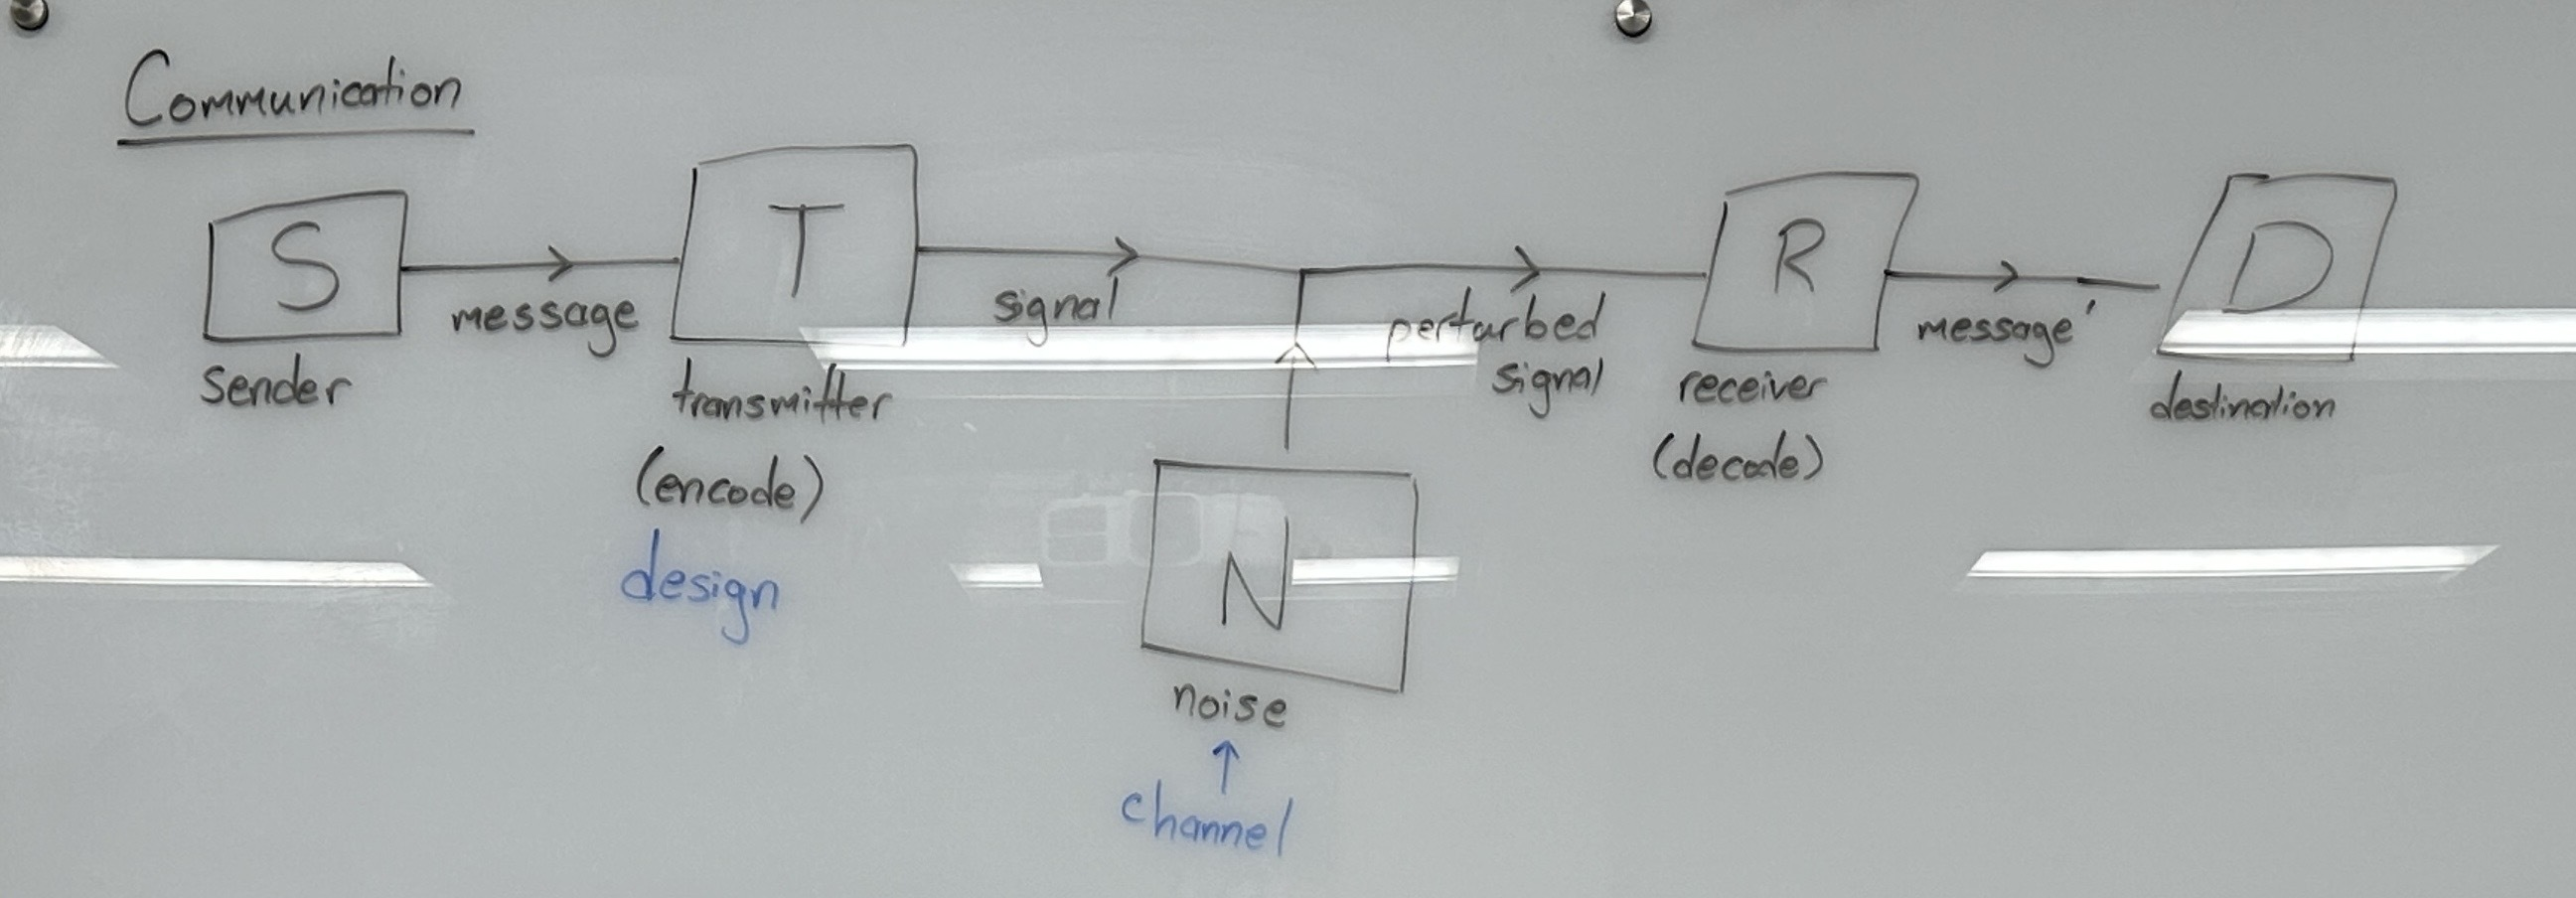
\includegraphics[scale=0.18]{lectures/wk1/img/communication.png}
    % \caption{Caption}
    % \label{fig:enter-label}
\end{figure}

which consists of the following entities:
\begin{itemize}
    \item Sender: you
    \item Message: What you want to send
    \item Signal: What you actually sent
    \item Transmitter: a function that encodes messages to signals
        \begin{itemize}
            \item This is a design question: we want to make it so that the perturbed signal can be decoded with minimal error
        \end{itemize}
    \item Source of Noise: different depending on how the channel works, but fixed to the type of channel
    \item Perturbed signal: signal + noise
    \item Receiver: they decode the perturbed signal to get message' which is then sent to the destination 
\end{itemize}

\subsection{Channel Capacity}
\begin{defn}{Channel Capacity}
$\max$ over possible encodings of the rate at which we can send information (messages) with low error.

What is the rate that you can send signals?
\end{defn}

\textit{Statistical} Information: Does not care about content of the message — instead: How many encodings can be represented?\\
This is as opposed to being length-agnostic where panther has more info than animal.

Problem: observe \( Y=y \), estimate the original \( X \) given \( Y=y \) related by conditional distribution of \( X|Y=y \)

\begin{itemize}
    \item Prior: \( P(X = x) \)
    \item Posterior: \( P(X = x | Y = y) \)
    \item Likelihood: \( P(Y = y | X = x) \)
\end{itemize}

Posterior \( \propto \) Likelihood \( \times \) prior, where alpha means proportional to (there’s some factor in the denominator that we are not caring about).

Information: The reduction of uncertainty regarding what was sent given what was received.
\begin{itemize}
    \item Regarding an unknown after an observation
\end{itemize}

But now we need to think how do we measure uncertainty in \( X \), \( H(X) \)?\\
We say \( U[X]=U(p) \) is a functional:
\begin{itemize}
    \item \( f \rightarrow I[f] \) is equivalent to \( \int f \)
\end{itemize}
Then we can think about the uncertainty in \( X \) after an observation, \( H(X | Y=y) \).\\
Finally we could average over all possible received messages to define:
\[ I(X; Y=y) = H(X) - H(X | Y=y) \]

We want a function that is a measure of uncertainty that is symmetric/invariant over all possible choices of labels (i.e. random variables).

\subsection{Extrinsic vs Intrinsic Measures}
Extrinsic measures: Depends on a realization of probability space (i.e. variance). You are measurable.
\begin{itemize}
    \item Depends on how you label your outcomes.
    \begin{itemize}
        \item This is useful if you lost your keys in 1 of 3 places and want to know the name of the place where you lost your keys
    \end{itemize}
    \item Traditional Statistics
    \item Functions of, expectation of random variables.
\end{itemize}

Intrinsic measures: Information Theory is the best example of this with uncertainty.
\begin{itemize}
    \item Depends only on the probability space, the set of outcomes, list of probabilities. Example: \( p=[p_1, p_2, \ldots, p_\Omega] \)
    \item \( U(p) \) is permutation invariant. That is, \( U[p]=U[p'] \).
    \begin{itemize}
        \item This is good if you want to know \( P[\text{err} | b] \) and don’t want the answer to be dependent on ‘a’ being before ‘b’
        \item Also makes sure the same statement in English vs French vs etc. gives the same entropy.
    \end{itemize}
\end{itemize}

\subsubsection{When does Intrinsic matter more than extrinsic?}
\begin{itemize}
    \item Suppose that \( X \) is a random variable with finitely many discrete \& distinct outcomes, which takes on integers \( \geq -1 \).
    \item Also suppose we can get exact answers to questions of the form: is \( X > \alpha \) for any \( \alpha \).
    \item How many answers do I need on average to know the value of \( X \).
\end{itemize}

You can scale the labels (dilate the graph out horizontally) which would change extrinsic measures but not intrinsic measures. \( \text{Var}(aX) \neq \text{Var}(X) \) but our Intrinsic question above does not care.
 
    \section{Thursday, January 18th}
\subsection{Basic Definitions and Concepts}

Let \( \Omega = \{\text{set of all positive outcomes}\} \), \( w_j \in \Omega \) where \( w_j \) is a randomly chosen outcome.

Let \( |\Omega| = \) number of possible outcomes.

Let \( X(w_j) = x_j \), \( X: \Omega \rightarrow \mathcal{X} \) (our representation).

Let \( \Pr(w=w_j)=\Pr(X=x)=p_j \).

\begin{defn}{Intrinsic Functional}
An intrinsic functional is defined as \( U[X] = U(p) \), where \( U: \Delta_{|\Omega|} \rightarrow \mathbb{R} \)

Where \( \Delta_n \) is the simplex which is \( \{p \in \mathbb{R}^n , p_i \geq 0 \forall i \text{ and } \sum_{I=1}^n p_i = 1\} \) which geometrically looks like this image:
\begin{figure}[H]
    \centering
    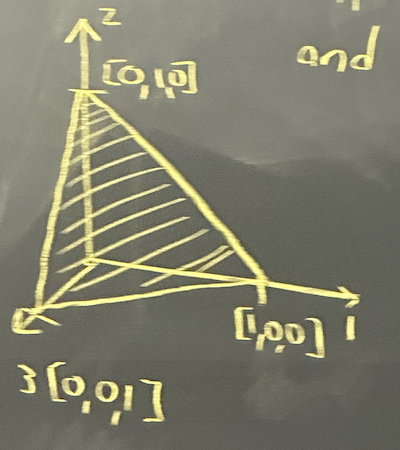
\includegraphics[scale=0.6]{lectures/wk1/img/simplex.png}
    \caption{Here we see a 3D-Simplex: a tetrahedron}
    \label{fig:simplex}
\end{figure}
\end{defn}

\subsection{Shannon Axioms}

\begin{defn}{Shannon Axioms}
Shannon axioms for a functional \( U: \Delta_n \rightarrow \mathbb{R} \), intrinsic:
\begin{itemize}
    \item Regularity/smoothness: \( U(p) \) is continuous in \( p \).
    \begin{itemize}
        \item Allows us to take limits: \( \lim_{x} f(x) = f(\lim_{x} x) \).
    \end{itemize}
    \item If \( p = [\frac{1}{n}, \ldots, \frac{1}{n}] \) ~ Uniform[\( n \)], \( |\Omega|=n \), then \( U(p) \) is non-increasing in \( n \).
    \item Uncertainty in \( X \) = Uncertainty in \( Y \) + Expected Uncertainty in \( X \) given \( Y \), for any choice \( \{S_1, S_2, \ldots\} \).
\end{itemize}
\end{defn}

\subsection{Khinchin Axioms}

\begin{defn}{Khinchin Axioms}
Khinchin axioms for a functional \( U: \Delta_n \rightarrow \mathbb{R} \), intrinsic:
\begin{itemize}
    \item \( U \) is intrinsic.
    \item For a given \( |\Omega| \), \( U(p) \) is maximized when \( p = [\frac{1}{\Omega}, \ldots, \frac{1}{\Omega}] \) aka uniform.
    \item Adding impossible outcomes (\( p_j = 0 \)) shouldn’t change your measure of uncertainty \( U(p) \).
    \item Chain Rule: \( U[X, Y] = U[Y] + \mathbb{E}_Y(U[X|Y]) \)
    \begin{itemize}
        \item Sometimes \( \mathbb{E}_Y(U[X|Y]) \) is written (mistakenly) as \( U[X|Y] \).
    \end{itemize}
\end{itemize}
\end{defn}

\subsection{Berkeley’s List of Axioms}

\begin{defn}{Berkeley’s Axioms}
Berkeley’s list of axioms:
\begin{itemize}
    \item \( U(p)=0 \) if \( p = [0, 0, \ldots, 0, 1, 0, \ldots, 0] \)
\end{itemize}
\end{defn}

\subsection{Composition}

Composition: If we partition \( \Omega \) into mutually exclusive and collectively exhaustive subsets \( S_1, \ldots, S_\psi \). 
Then let \( X \) represent the outcome in some subset.
Let \( Y \) be an indicator for the set containing \( X \): \( Y=j \) if \( X \in S_j \)
This is backwards from last class: here we will observe \( Y \) and estimate \( X \) in 2 stages:
\begin{enumerate}
    \item Observe \( Y \), we find that \( X \) is contained in some say \( S_1 \), which tells us that we are contained in a certain subset — but there’s still some uncertainty. So now we:
    \item Observe \( X \) given \( Y=y \).
\end{enumerate}
We want \( U[X] = U[Y] + \mathbb{E}_y(U[X | Y=y]) \).

\subsection{Shannon's Entropy Theorem}
\begin{defn}{Shannon's Entropy Theorem}
Given either Shannon’s or Khinchin’s axioms then:
\[ U[X]=U(p)=H[X]=H(p)=\text{``Shannon’s Entropy’’} \]
\[ = -\sum_{\text{all } x \in \mathcal{X}} \Pr(X=x) \log_a(\Pr(X=x)) \]
\[ = -\sum_{j=1}^{|\Omega|} p_j \log_a(p_j) \]
\[ = \mathbb{E}_X[\log_a(1/\Pr(X=x))] \]
Where:
\begin{itemize}
    \item By convention \( p=0 \implies p\log(p)=0 \) which is known as continuity and is proved by L’Hôpital’s as \( p \rightarrow 0^+ \) addressing Khinchin Axiom 3: \( H[p]=H[[p, 0, 0, 0]] \) as impossible events have 0 uncertainty.
    \item \( a \) is an arbitrary base which is a choice of unit to measure units (it is not uniquely specified by the axioms).
    \begin{itemize}
        \item \( \log_2 \implies \) “bits”
        \item \( \log_3 \implies \) “ternary function”
        \item \( \ln \implies \) “nats”
        \item All of these are off by a scaling factor, as shown below,
    \end{itemize}
\end{itemize}
\end{defn}

\subsection{Logarithmic Change of Base for Entropy}
$$
\log _b a=\frac{\log _d a}{\log _d b}
\implies 
H_b(p) = \log_b(a) H_a(p).
$$

    \section{Tuesday, January 23rd}
Here is the text converted into valid LaTeX, assuming that the `important` environment and `mdframed` package are already defined in your LaTeX document preamble:

```latex
\subsection{Shannon Entropy}

We will start with the definition of Shannon Entropy.

We say an uncertainty functional \( U[X] \) satisfying either Shannon or Khinchin's axioms must be a Shannon Entropy, \( U[x]=H_a[X]=- \sum_{\text{all } x \in \mathcal{X}} p(x) \log_a(p(x)) = \mathbb{E}_X[\log_a(1/p(x))] \) where \( a \) is the choice of units.

\subsubsection{Properties of Entropy}
\begin{itemize}
  \item It is intrinsic: Entropy will be symmetric under a certain reflection.
  \item Entropy is bounded below: \( H[X] \geq 0 \) with equality if and only if \( \exists x \) such that \( p(x)=1 \).
  \item The discrete Entropy is bounded above: \( H[X] \leq \log_a(|X|) \) with equality if and only if \( X \) is distributed uniformly with \( H[X]=\log_a(n)=1 \).
  \item \( H(p) \) is continuous in \( p \) (also differentiable in \( p \) if we throw out impossible events).
  \begin{itemize}
      \item So that our uncertainty doesn’t jump around so that we can have convergence.
      \item You can think about all of your outcomes as groups of the smallest denominators.
  \end{itemize}
  \item \( H(p) \) is a concave function of \( p \).
  \item Chain Rule: \( H[X, Y] = H[Y] + H[X | Y] = H[X] + H[Y | X] \)
  \begin{itemize}
      \item Uncertainty in the joint = Uncertainty in the marginal + Uncertainty in the conditional.
      \item We only observe \( Y \) first + \( \mathbb{E} \) [uncertainty left over] where the latter term is the definition of conditional entropy.
  \end{itemize}
\end{itemize}

\subsubsection{Other Entropies}
\begin{itemize}
\item \textbf{Definition}: Joint Entropy \\
Given \( X, Y \) with distribution \( p(., .) \), then \\
\( H[X, Y] = \mathbb{E}_{X, Y}[\log_a(1/p(X, Y))] = -\sum_{\text{all } x, \text{all } y} \log_a(p(x, y)) \).

\item \textbf{Definition}: Conditional Entropy given an observation. \\
Given \( X, Y \) with distribution \( p(., .) \), then \\
\( H[X | Y=y] = \mathbb{E}_{X | Y=y}[\log_a(1/p(X | Y=y))] \).

\item \textbf{Definition}: Conditional Entropy \\
Given \( X, Y \) with distribution \( p(., .) \), then
\[ H[X | Y] = \mathbb{E}_Y[H[X | Y=y]] = \mathbb{E}_{X | Y}[\log_a(1 / p(X | Y))] \].

\item \textbf{Alternate}:
\begin{flalign*}
U[X] = \mathbb{E}_X[1 - p(X)]  \\
&= 1 - \mathbb{E}_X[p(X)] \text{ by linearity}  \\
&= 1 - \sum_x p(x) p(x)  \\
&= 1 - \sum_x p(x)^2  \\
&= 1 - \Pr(X_1 = X_2)  \\
&=  \Pr(X_1 \neq X_2)
\end{flalign*}
for i.i.d. \( X_1, X_2 \sim p \).
\end{itemize}

Now we will consider what will happen if we relax the chain rule:
\[ X \text{ independent of } Y \implies H[X | Y] = H[X] \]
\[ \implies H[Y | X] = H[Y] \]
\[ \implies H[X, Y] = H[X] + H[Y] \]
We will call the three equations above (*).

\textbf{Fact we will prove in the future}:
\[ H[X] = \text{Var}(X) \text{ for } X \sim \mathcal{N}(\mu, \sigma) \]

\textbf{Theorem}: If we replace the chain rule with equation (*) in Khinchin’s axioms, then
\[ U[X] = H_a^{(\alpha)}[X] \]
Where:
\[ H_a^{(\alpha)}[X] = \frac{1}{1 - \alpha} \log_a \left(\sum_x p(x)^\alpha \right) = \frac{\alpha}{1 - \alpha} \log_a \left( ||[p_1, \ldots, p_{|X|}]||_\alpha \right) \]
is known as Rényi Entropy.

If we take \( \alpha \to 0 \) then we get Hartley Entropy: \( H_a^{(0)}[X] = \log_a(|X|) \).

If we take \( \alpha \to 1 \) then we get Shannon Entropy.

If we take \( \alpha \to 2 \) then we get the Coincidence/Collision Entropy: \( H_a^{(2)}[X] = \log_a \left( \frac{1}{\sum_x p(x)^2} \right) = \log_a \left( \frac{1}{\Pr(X_1 = X_2)} \right) \).

If we take \( \alpha \to n \geq 1 \) then we get:
\[ H_a^{(n)}[X] = \frac{1}{n - 1} \log_a \left( \frac{1}{\Pr(X_1 = X_2 = \ldots = X_n)} \right) \].

If we take \( \alpha \to \infty \) then we get:
\[ H_a^{(\infty)}[X] = \log_a \left( \frac{1}{\max_{x \in X} p(x)} \right) \].

\subsubsection{Information}

\textbf{Information}: The reduction of uncertainty after an observation. The mutual information between \( X \) and \( Y \) is defined as
\[ I(X; Y) = \mathbb{E}_Y[H[X] - H[X | Y=y]] = H[X] - \mathbb{E}_Y[H[X | Y=y]] = H[X] - H[X | Y] \]
I am asking about \( X \) when I am observing \( Y \).

The information \( Y \) carries about \( X \) is the uncertainty in \( X \) before observation minus the expected uncertainty in \( X \) after observation.

\subsubsection{Properties of Information}
\begin{enumerate}
    \item Self-Information:
    \begin{itemize}
        \item \textbf{Lemma}: \( I(X; X) = H[X] \). This follows from the definition of information with the fact that \( H[X | X=x] = 0 \) which implies \( H[X | X] = 0 \) since there is zero expected surprise after observing itself.
        \item If we identify an outcome then we’ve learned everything there is to know about it. The amount of information equals the original uncertainty.
    \end{itemize}
    \item Independent: \( I(X; Y) = \) prior - posterior \( = H[X] - H[X | Y] = H[X] - H[X] = 0 \).
    \item \( I(X; Y) = I(Y; X) \), the information X carries about Y is the same as the information Y carries about X.
    \begin{itemize}
        \item Proof: \( I(X; Y) = H[X] - H[X | Y] = H[X] - (H[X, Y] - H[Y]) = H[X] + H[Y] - H[X, Y] = I(Y; X) \).
    \end{itemize}
\end{enumerate}

    \section{Thursday, January 25th}
\section*{Information Theory}

Last time we defined information:
\begin{equation*}
I(X; Y=y) = H[X] - H[X | Y=y]
\end{equation*}
and mutual information as the expected information before making the observation:
\begin{equation*}
I(X; Y) = \mathbb{E}_y[I(X; Y=y)].
\end{equation*}
We called this mutual information because of the third property covered last lecture.

\subsection{Relative Entropy}
Relative Entropy, also known as KL Divergence, is defined as:
\begin{equation*}
D(p || q) = \mathbb{E}_{x \sim p}[\log(p(x)/q(x))].
\end{equation*}

\subsection{Mutual Information is a KL Divergence}
\begin{equation*}
I(X; Y) = I(Y; X) = D(p_{X, Y} || p_X p_Y) = \mathbb{E}_{X, Y}[\log(p(X, Y)/(p(X)p(Y)))].
\end{equation*}
Here, \( p_X p_Y \) is the product distribution where \( p(X=x) p(Y=y) \).

\subsection{Convex Functions}
A function is convex if it lies beneath any chord of the function. For a convex combination (meaning \( p_1 + p_2 = 1 \)) \([p_1, p_2] \in \Delta_2\) which is the simplex in 2 dimensions, we have:
\begin{equation*}
p_1 f(x_1) + p_2 f(x_2) \geq f(p_1 x_1 + p_2 x_2).
\end{equation*}
And the expected value of \( f(X) \) is:
\begin{equation*}
\mathbb{E}_{X \sim [x_1, x_2] \text{ with probability } [p_1, p_2]}[f(X)] \geq f(\mathbb{E}[X]).
\end{equation*}
We have strict convexity if we have a strict inequality.

\subsection{Jensen's Inequality}
Generalizing to any dimension, we get Jensen's inequality:
If \( f \) is convex, for any distribution \( p \),
\begin{equation*}
\mathbb{E}_{X \sim p}[f(X)] \geq f(\mathbb{E}_{X \sim p}[X]).
\end{equation*}

\subsubsection{Proof via Induction}
\begin{Answer}
We can prove Jensen's inequality via induction:
\begin{itemize}
    \item Base Case: \( n=2 \), see above.
    \item Inductive Step: Assume Jensen's holds for \( n=k \).
    \item Inductive Conclusion: Show that Jensen's for \( n=k \) implies Jensen's for \( n=k+1 \).
    \begin{align*}
    \mathbb{E}_{X \sim p \text{ which is } k+1 \text{ outcomes}}[f(X)] &= \sum_{j=1}^{k+1} p_j f(x_j) \\
    &= \sum_{j=1}^{k} p_j f(x_j) + p_{k+1} f(x_{k+1}) \\
    &= \left(\sum_{m=1}^{k} p_m\right) \sum_{j=1}^{k} \left[\frac{p_j}{\sum_{m=1}^{k} p_m} f(x_j)\right] + p_{k+1} f(x_{k+1}) \\
    &\geq (1 - p_{k+1}) f\left(\mathbb{E}_{X \neq X_{k+1}}[X]\right) + p_{k+1} f(x_{k+1}) \\
    &= f\left(\sum_{j=1}^{k+1} p_j x_j\right) = f(\mathbb{E}[X]). \text{ QED.}
    \end{align*}
\end{itemize}
\end{Answer}

\subsection{Information Inequality}
The information inequality states that \( I(X; Y) \geq 0 \). The proof is as follows:
\begin{align*}
I(X; Y) &= D(p_{X, Y} || p_X p_Y) \\
&= \mathbb{E}_{X \sim p}[\log(p(x)/q(x))] \\
&= \mathbb{E}_{X \sim p}[-\log(q(x)/p(x))] \\
&= \mathbb{E}_{Y}[-\log(Y)] \quad \text{where} \quad Y(X)=\frac{q(x)}{p(x)} \text{ is convex, so by Jensen's Inequality,} \\
&\geq -\log(\mathbb{E}_{X \sim p}[q(x)/p(x)]) \\
&= -\log(\sum_x p(x) \cdot \frac{q(x)}{p(x)}) \\
&= -\log(\sum_x q(x)) \\
&= -\log(1) = 0. \quad \text{QED.}
\end{align*}

    \section{Tuesday, January 30th}
\subsection{End of Unit 1: Three Inequalities}
We start by ending unit 1 with three inequalities:
\begin{enumerate}
    \item \(H[X] + H[Y] \geq H[X, Y]\)
    \begin{itemize}
        \item Interpretation: Joint entropy of independent \(X, Y\) is greater than or equal to the joint entropy of \(X, Y\).
        \item Equality requires: Independence between \(X\) and \(Y\).
        \item Proof: \(H[X] + H[Y] \geq H[X, Y] \implies H[X] + H[Y] \geq H[Y] + H[X | Y] \implies H[X | Y] \leq H[X] \implies 0 \leq H[X] - H[X | Y] \implies I(X; Y) \geq 0\), proved yesterday.
    \end{itemize}
    \item \(H[X | Y] \leq H[X]\)
    \begin{itemize}
        \item Interpretation: Observation reduces uncertainty.
        \item Equality requires: Independence between \(X\) and \(Y\).
        \item Proof: \(H[X | Y] \leq H[X] \implies 0 \leq H[X] - H[X | Y] \implies I(X; Y) \geq 0\), proved yesterday.
    \end{itemize}
    \item \(H[X | Y] + H[Y | X] \leq H[X, Y]\)
    \begin{itemize}
        \item Interpretation: Joint entropy of \(X, Y\) is greater than or equal to the expected uncertainty in one given the other.
        \item Equality requires: Independence between \(X\) and \(Y\).
        \item Proof: \(H[X | Y] + H[Y | X] \leq H[X] + H[Y | X] = H[X, Y]\), where we first use 2, then chain rule.
    \end{itemize}
\end{enumerate}

\subsection{Motivating Question: Why the log?}
To answer this, we will play a game of 20 questions:
    \begin{enumerate}
        \item What are the most efficient questions to ask?
        \item How efficient is it?
    \end{enumerate}

\subsection{Now we play a game:}
\begin{itemize}
    \item Q1: Is it alive? Yes, which we denote as \(Y_1 = 1\).
    \item Q2: Is it an animal? Yes, which we denote as \(Y_2 = 1\).
    \item Q3: Is the word 2 syllables? Yes, which we denote as \(Y_3 = 1\).
    \item Q4: Is it a Narwhal? No, which we denote as \(Y_4 = 0\).
    \item Q5: Does it live in the ocean? No, which we denote as \(Y_5 = 0\).
    \item Q6: Is it an egret? No, which we denote as \(Y_6 = 0\).
    \item (Answer: It was a rabbit).
\end{itemize}

\begin{figure}[H]
    \centering
    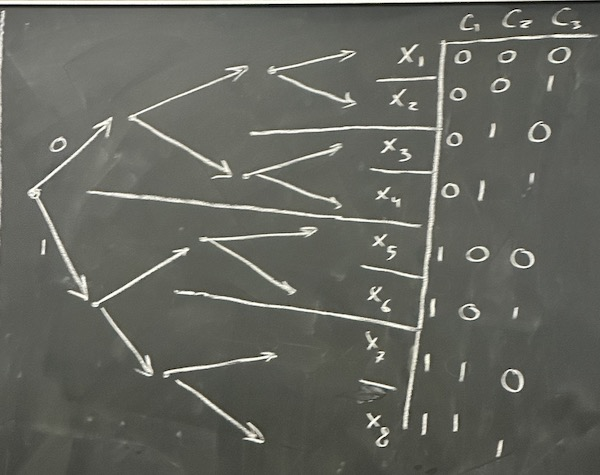
\includegraphics[scale=0.8]{lectures/wk3/img/binary_tree.jpeg}
    % \caption{Caption}
    % \label{fig:enter-label}
\end{figure}

\subsection{Motivating Question: Random Number Generation}
Given an RNG:
\begin{enumerate}
    \item How to efficiently process/transform randomness?
    \item How efficient?
\end{enumerate}


If we have \( |\mathcal{X}| = n \) outcomes, then we represent \( d^m = n \), which requires a length \( l = \lceil \log_d(n) \rceil \).

Suppose \( |\mathcal{X}| = n \), \( p \in \Delta_n \), \( p = [p_1, p_2, \ldots, p_n] \), \( p_j \geq 0 \), \( \sum_{j=1}^m p_j = 1 \), a sequence of approximations \( \{\tilde{p}^{(k)}\}^\infty \), if \( \lim_{k \to \infty} \tilde{p}^{(k)} \to p \), then, \( U(\tilde{p}^{(k)}) \to U(p) \) as \( k \to \infty \).

Restrict \( \tilde{p}^{(k)} \) to be rational, as they are dense in reals. This allows us (per the Chain Rule) to group microscopic events into macroscopic ones.

There's an equivalence between search trees and coding. In either case, you naturally get a logarithmic measure (from the depth of the tree).

    \section{Thursday, March 1st}
\subsection{The Emergence of the Logarithm in Information Theory}

Today we will show that the logarithm appears due to the smoothness/continuity axiom as well as the chain rule axiom. Given the assumption of continuity, we know that the (microscopic event model — from thermodynamic statistical mechanics). If \( p=[5/8, 1/4, 1/8] \).

\subsection{Optimizing Codings and Tree Representations}

Then we will look at optimizing codings/tree representations of encoding and bounds on the best you can do:
\begin{itemize}
    \item Kraft's Inequality
    \item Entropy as efficiency bound
    \item Towards optimality…
\end{itemize}

\subsection{The Chain Rule and Its Implications}

If groups of \( Y \) filter to a unique \( X \), \( Y \sim \text{Unif}[1, M] \), \( X=x(Y) \). Then \( U[X, Y] = U[Y] = U[X] + U[Y | X] \). But we have asymmetry:
\[ U[X] = u(M) - \sum_j P(X = x_j) \cdot u(m_j) \]
thus \( U[\cdot] \) isn't specified by how \( u \) behaves on equally likely outcomes.

We define \( \{u(m)\} = U[\text{uniform dist. over } m \text{ outcomes}] \). Suppose \( m=kl \), \( m,k,l \in \mathbb{Z} \).
e.g., \( m=10 \), \( k=5 \), \( l=2 \). Then we can partition the top row of \( m=10 \) events into \( l=2 \) sets which each contain \( k=5 \) things. Chain rule: \( u(m) = u(kl) = U[X] + U[Y | X] \)
\[ = u(l) + \mathbb{E}_x [U(Y | X= x)] \]
\[ = u(l) + \mathbb{E}_x [u(k)] = u(k) + u(l) \].
\[ u(m) = u(kl) = u(k) + u(l) \].

\( u=\log \) is then forced upon us as logs turn multiplication into addition.

Or more rigorously, suppose \( m= D^l \) for some \( D, l \in \mathbb{Z} \), e.g., \( m=8 \) equally likely things. This can be done as 4 sets, each of size 2, which using the chain rule gives us that \( u(D^{l-1}) + u(D) \). 
We can then recurse, each time lowering the largest exponent (which was originally \( l \)) by 1. This means the depth of our tree will be \( l \).
\[ u(m) = u(D^l) = u(D \cdot D^{l-1}) = u(D^{l-1}) + u(D) = u(D^{l-2}) + u(D) + u(D) = \ldots = l \cdot u(D) + u(1) \]
and we know that \( u(1)=0 \) per Khinchin’s Axiom.
Now we have \( u(D^l) = l \cdot u(D) \), which we also could’ve got without the axiom if we only recurse \( l-1 \) times as \( u(D^{l-(l-1)})=u(D) \). Thus \( u(D^l) = \log_D(m) \cdot u(D) = m=D^l \),
then it must be true that \( U[\text{uniform distribution over } |X|] \) is proportional to \( \log(|X|) \).

\subsection{Coding}

A set of \( \mathcal{X} \) represents, \( X \in \mathcal{X} \), \( X \sim p \), \( |X| < \infty \) (we extend in the textbook to countably infinite sets).
Define: a code \( C: \mathcal{X} \mapsto D^k \), where:
\begin{enumerate}
    \item \( D^* = \) \{set of all possible strings with symbols in a \( d \)-ary alphabet\}
    \item \( c(x) = \) codeword for \( x \), e.g., \( c(x) = 0110 \) ⟺ each symbol is specifying a choice in the tree
    \item \( l(x) = |c(x)| = \) length of codeword = number of symbols used ⟺ number of questions answered = the length of the path
\end{enumerate}
Define: \( L = \mathbb{E}_{X \sim p}[l(X)] \quad\iff\) \text{ average number of steps needed.}

\subsection{Instantaneous Codes (Prefix Codes)}

\begin{itemize}
    \item A mapping \( \{x_1, x_2, x_3, x_4, \ldots\} \mapsto C^* \) where \( C(\{x_1, x_2, x_3, \ldots\}) = c(x_1) c(x_2) c(x_3) \ldots \)
    \item Non-singular: \( x \neq x' \implies c(x) \neq c(x') \)
    \item No prefixes: No codeword is the prefix of another, meaning all codewords are leaves of the tree.
    \item Example: \( c(x_1) = [0, 0, 1] \), \( c(x_2) = [0, 0, 1, 1] \)
\end{itemize}

We can draw a binary tree with 0 as up and 1 as down, to represent this coding scheme.

\subsection{Kraft's Inequality}

Kraft's inequality states that for a finite or countably infinite set of outcomes \( \mathcal{X} \) you want to encode, and a \( D \)-ary dictionary, then all instantaneous codes must satisfy:
\[ \sum_{i=1}^n D^{-\ell_i} \leq 1. \]

Conversely, for any given set of natural numbers \( \ell_1, \ell_2, \ldots, \ell_n \) that satisfy the above inequality, there exists a uniquely decodable code over an alphabet of size \( D \) with those codeword lengths. This applies to all uniquely decodable codes, which include instantaneous codes.

Even better, there's a recipe to build such a code!

\subsection{Quiz Time!}

\emph{This section is left intentionally blank for the quiz content.}

    \section{Tuesday, February 6th}
\subsection{Kraft's Inequality and Code Construction}
Kraft’s inequality points to an explicit construction. The action of us being able to actually construct it gives us an application from the inequality. Today we will prove it for \( |\mathcal{X}| < \infty \), instantaneous codes, list of lengths \( \ell=\{\ell_1, \ell_2, \ldots, \ell_{|\mathcal{X}|}\} \). 
This is a code without prefixes so you don’t have to wait until you get the full code to realize if you have an antecedent or a child. Thus all messages are at leaves.

This is most interesting when all the paths do not have the same lengths. We assign outcomes to some leaves, but not all possible leaves (a fact which is key for the inequality of Kraft), since we didn’t say in our encoding that all leaves should be used so we can skip some leaves if the answer to the question is only ever one answer. The usefulness of this is seen more easily in tertiary or higher trees. Now if we denote \( \ell_{\max} = \max_x\{\ell(x)\} \).

If we completed the tree then we would have \( D^{\ell_{\max}} \) leaves on the \( \ell_{\max} \) ‘vertical bar’ if we draw the tree horizontally. 

\begin{shaded}
\textbf{Question:} If we take a stopping node, at depth \( \ell \), how many children would it have had at depth \( \ell_{\max} \)?
\end{shaded}

\textbf{Answer:} \( D^{\ell_{\max} - \ell} \).

Expanding on this, if we sum over every \( x \), we get the following inequality: \( \sum_x D^{\ell_{\max} - \ell(x)} \leq D^{\ell_{\max}} \). Dividing both sides by \( D^{\ell_{\max}} \) gives Kraft’s inequality.

\subsection{Constructive Approach}

Let’s go through an example:
Given a binary tree with \( \ell = \{1,2,4,4\} \), this satisfies Kraft’s inequality with the sum being \( \frac{7}{8} \) which tells us we are inefficient.

\begin{center}
\begin{tabular}{c c}
X & c(x) \\
\hline
1 & 0 \\
2 & 10 \\
3 & 1100 \\
4 & 1101 \\
\end{tabular}
\end{center}

\textbf{Claim:} If \( X \sim p \), \( X \in \mathcal{X} \), \( |\mathcal{X}| < \infty \).

\begin{itemize}
    \item Let \( L = \mathbb{E}_X[\ell(X)] \).
    \item Over all \( \ell=\{\ell_1, \ell_2, \ldots, \ell_{|\mathcal{X}|}\} \) such that Kraft’s inequality is satisfied then, for any code (i.e., any \( \ell \)’s satisfy) \( L \geq H_D[X] \).
\end{itemize}

\textbf{Proof:}
\begin{align*}
L - H_D[X] &= \mathbb{E}_X[\ell(x) + \log_D(p(X))] \\
&= \mathbb{E}_{X \sim p}[\log_D(p(x) / D^{-\ell(x)})] \quad \text{which resembles a relative entropy}
\end{align*}
Define \( q(x) = D^{-\ell(x)} / Z \), where \( Z = \sum_x D^{-\ell(x)} \leq 1 \),
\begin{align*}
&= \mathbb{E}_{X \sim p}[\log_D(p(x) / (q(x) \cdot Z))] \\
&= \mathbb{E}_{X \sim p}[\log_D(p(x) / q(x)) - \log_D(Z)] \\
&= D(p || q) - \log_D\left(\sum_x D^{- \ell(x)}\right) \\
&\geq 0 \quad \text{since both } D(p || q) \geq 0 \text{ and } -\log_D\left(\sum_x D^{- \ell(x)}\right) \geq 0. \\
&\implies L \geq H_D[X]. \quad \text{QED.}
\end{align*}

We want short codewords to correspond to likely events and vice versa. Mathematically: \( D^{- \ell(x)} \approx p(x) \).

\subsection{Small Group Activities: Programming \& Fano Codes}

Now in small groups, we will tackle three activities:

\begin{enumerate}
    \item Show that the bounds are tight (can be achieved by some scheme) and what is the cost of misspecification? (What is the smallest expected code length using the Shannon code for the wrong prior?)
    \begin{itemize}
        \item We have no inefficiency if \( \sum_x D^{- \ell(x)} = \sum_x p(x) = 1 \implies \log_D\left(\sum_x D^{- \ell(x)}\right) = 0 \implies \ell(x) = -\log_D(p(x)) \). But \( \ell \) may not be an integer, so we will want to round up so we don’t exceed our bound, thus \( \ell(x) = \lceil -\log_D(p(x))\rceil \). If we define \( H_D[X] \leq L^* = \min_C \{ \mathbb{E}_X[\ell(X)] \} \leq \mathbb{E}_X[\lceil -\log_D(p(x))\rceil] \)
        \[ < \mathbb{E}_X[-\log_D(p(x))] + 1 \quad \text{since} \quad \lceil -\log_D(p(x))\rceil < -\log_D(p(x)) + 1 \]
        \[ = H_D[X] + 1. \]
        We can replace the 1 with \( \frac{1}{n} \) by amortizing the wasted bit spread over \( n \) bits, encoded at once.
        \item This is known as a Shannon code: assigning short codes to likely events, long codes to unlikely events: \( \ell(x) \approx -\log_D(p(x)) \).
    \end{itemize}
    \item Design an optimal code (Huffman) for English words (see data on bcourses).
    \begin{itemize}
        \item Let’s start by testing the difference between \( L = \mathbb{E}_X[\ell(x)] \) and \( H_2[X] \), which just means the base 2 entropy.
        \item This is known as a Huffman code: Save the last bit/question for the least likely events.
    \end{itemize}
    \item Challenge: given \( \{X_1, X_2, \ldots\} \), \( X_i \stackrel{\text{iid}}{\sim} \text{Bernoulli}(p, 1-p) \) design a mapping \( f: X \to Y \) (where \( Y=f(X) \)) such that:
    \begin{itemize}
        \item \( \{Y_1, Y_2, \ldots\} \), \( Y_j \stackrel{\text{iid}}{\sim} \text{Bernoulli}\left(\frac{1}{2}, \frac{1}{2}\right) \)
        \item Maximizing efficiency: \( \eta = \frac{\mathbb{E}[\text{number of output bits, } |Y|]}{|X|} \) where \( |X| = \) number of unfair bits
        \item That works and is optimal for all \( p \in [0, 1] \).
        \item This is known as a Fano code: maximize expected information gain per question/bit.
    \end{itemize}
\end{enumerate}

    \section{Thursday, February 8th}
\subsection{Logistics}

\begin{itemize}
    \item Refined learning goals due February 15.
    \item Quiz 2 (on Coding + AEP) next Thursday.
\end{itemize}

\subsection{Three Perspectives on Entropy}

We will start with three perspectives on Entropy:

\begin{enumerate}
    \item Compression: The shortest description.
    \item Randomness: A measure of randomness that cannot be created by any deterministic processing.
    \item Typically (the AEP): Typical events have \( \log(p) \approx \) entropy.
\end{enumerate}

\subsection{Efficiency}

Mappings: \( Y = f(X) \)

Efficiency is given by the formula:
\begin{equation*}
    \eta(f \,|\, |X| = \mu, p) = \eta(f; |X| = \mu, p) = \frac{\mathbb{E}[|Y|]}{m} = \frac{\mathbb{E}[|f(X)|]}{m}
\end{equation*}

\textbf{Question:} What is the maximum of \( \eta \) subject to \( f \)?

``Uncertainty in the output \( \leq \) uncertainty in the input.''

\begin{align*}
    H[X] &= H[X_1, \ldots, X_m] \\
         &= \sum_{j=1}^m H[X_j] \quad \text{by independence} \\
         &= m \cdot H[X_1] \quad \text{where } H[X_1] = H(p,1-p)
\end{align*}

Suppose \( Y \) is uniform over \( 2^n \):

\begin{align*}
    H[Y] &= H[|Y|] + H[Y \,|\, |Y|] \quad \text{by conditioning on } |Y| \\
         &= H[|Y|] + \mathbb{E}_n[H[Y \,|\, |Y|=n]] \\
         &= H[|Y|] + \mathbb{E}_Y[|Y|] \\
         &\leq H[X] \quad \text{Using the inequality proved below.} \\
         &= m \cdot H[X_1]
\end{align*}

This then allows us to say:
\begin{equation*}
    \eta = \frac{\mathbb{E}[|f(X)|]}{m} \leq H[X_1] - \frac{1}{m} H[|Y|]
\end{equation*}
which asymptotically makes the last term go to \( 0 \). Thus \( \eta \leq H[X_1] \).

\subsection{The Data Processing Inequality}

\textbf{Claim:} For any deterministic mapping \( f \), if we let \( Y = f(X) \), then the amount of randomness in \( Y \), \( H[Y] \leq H[X] \).

Suppose \( f \) is injective, which means unique inputs lead to unique outputs, then \( H[X] = H[Y] \) for any choice of labels.

Instead, we group inputs for a non-injective \( f \) (where \( f \) is not one-to-one). Then
\begin{align*}
    H[X] &= H[Y] + H[X \,|\, Y] \quad \text{and since } H[X \,|\, Y] \geq 0, \\
    &\text{we know that } H[X] \geq H[Y].
\end{align*}

\hrulefill

\subsection{Asymptotic Equipartition Property (AEP)}

The Asymptotic Equipartition Property (AEP) states that most sample \( n \)-sequences of an ergodic process have probability about \( 2^{-nH} \) and that there are about \( 2^{nH} \) such typical sequences. If \( X_1, \ldots, X_n \) and \( X_j \) are iid\textasciitilde \( p \):

\begin{equation*}
-\frac{1}{n}\log\left(\underbrace{p(X_1,\ldots,X_n)}_{p(X_1) \cdot \ldots \cdot p(X_n)}\right) \xrightarrow{\text{i.p.}}  H[X_1] \quad \text{as} \quad n \to \infty.
\end{equation*}

\begin{equation*}
-\frac{1}{n} \sum_{j=1}^n \log(p(x_j)) \to -\mathbb{E}_X[\log(p(X))].
\end{equation*}

\subsubsection{Typical Set}

The typical set \( A_{\varepsilon}^{(n)} \), if \( x_1, \ldots, x_n \in A_{\varepsilon}^{(n)} \) then \( x_1, \ldots, x_n \) is typical:

\begin{equation*}
A_{\varepsilon}^{(n)} = \left\{x_1, \ldots, x_n \mid -\log(p(x_1, \ldots, x_n)) \in [H[X] - \varepsilon, H[X] + \varepsilon]\right\}.
\end{equation*}

\subsubsection{Properties}

\begin{enumerate}
    \item \( \left|A_{\varepsilon}^{(n)}\right| \leq 2^{n(H[X]+\varepsilon)} \implies p(x_1, \ldots, x_n) \in [2^{-n(H[X] + \varepsilon)}, 2^{-n(H[X] - \varepsilon)}] \) which can be read as: "elements of the typical set are all \( \mathcal{X} \) equiprobable"
    \item \( \Pr\left[x^{(n)} \in A_{\varepsilon}^{(n)}\right] \geq 1-\varepsilon \equiv \Pr\left[x_1, \ldots, x_n \in A_{\varepsilon}^{(n)}\right] \xrightarrow{n \to \infty} 1 \) for any \( \varepsilon > 0 \) with high probability.
    \item \( \left|A_{\varepsilon}^{(n)}\right| \in [(1-\varepsilon) 2^{n(H[X] - \varepsilon)}, 2^{n(H[X] + \varepsilon)}] \) for \( n \) sufficiently large.
\end{enumerate}

\subsubsection{Typicality}

If \( X_1, \ldots, X_n \) and we let \( H \) be the number of heads.

\begin{equation*}
p(x_1, \ldots, x_n) = p^{h(x)} (1-p)^{n - h(x)}
\end{equation*}

\begin{equation*}
\log(p(x_1, \ldots, x_n)) = \log\left(p^{h(x)} (1-p)^{n - h(x)}\right) = h(x)\log(p) + (n - h(x)) \cdot \log(1 - p)
\end{equation*}

Typicality cares about the multiplicity of outcomes.

    \section{Tuesday, February 13th}
\subsection{Goals/Main Question: Is Differential Entropy still intrinsic?}
\begin{itemize}
    \item Is Differential Entropy extrinsic?
    \item Defn.:
\end{itemize}
\begin{defn}{Differential Entropy}
Given \( X \sim f_X \), then \( h[X] = h(f_X) \).
\end{defn}

\subsubsection{Side-by-Side comparison: Discrete vs Differential Entropy}
\begin{description}
    \item[Discrete:] 
    \begin{align*}
    H[X] = H(p) &= -\mathbb{E}_X[\log(p(X))] &&\text{ where } X \sim p \\
        &= -\sum_{x \in \mathcal{X}} p(x)\log(p(x))
    \end{align*}
    which we see is intrinsic.
    
    \item[Differential:] 
    \begin{align*}
    H[X] = h(f_X) &= -\mathbb{E}[\log(p(X))] &&\text{ where } X \sim f_X \\
        &= -\displaystyle\int_{x \in \cX} f_X(x) \log(f_X(x)) \, \d x
    \end{align*}
    which we see is extrinsic.
\end{description}

\subsubsection{Example with Differential Entropy}
\begin{description}
    \item[Example:] \( X \sim f_X \), \( X \in \cX \subseteq \mathbb{R} \)
    \begin{itemize}
        \item Let \( Y = aX \), then \( f_Y(y) = f_X\left(\frac ya\right) \cdot |a| \)
        \item Then 
        \begin{align*}
        h[aX] &= h[Y] \\
              &= \mathbb{E}_Y[\log(f_Y(Y))] \\
              &= \mathbb{E}_X[\log(f_X(X/a) |a|)] \\
              &= \mathbb{E}_X[\log(f_X(X)) + \log(|a|)] \\
              &= h[X] + \log(|a|)
        \end{align*}
    \end{itemize}
\end{description}

\hrulefill

\subsection{Axiomatic Approach}

\begin{itemize}
    \item \underline{Assume}: \( X \) is continuous and \( f_X \) is continuous on $\cX$.
    \item Definition: \( X^{(n)} \xrightarrow{n \to \infty} X \) i.i.d. if the density \( f_{X^{(n)}} \to f_X \), pointwise almost everywhere (a.e.).
\begin{defn}{``Weak convergence''}
  \( \mathbb{E}[g(X^{(n)})] \to \mathbb{E}[g(X)] \) as \( n \to \infty \).  
\end{defn}
\end{itemize}

\subsubsection{Axioms}
\begin{enumerate}
    \item[(i)] Axiom 1: We want \( h \) to be continuous; we want \( h[X^{(n)}] \to h[X] \), if \( X^{(n)} \to X \) in distribution.
\begin{shaded}
Defn.:
\begin{itemize}
\item \(Z^{\Delta X}\) be drawn.
\begin{enumerate}
    \item Draw $Y^{\Delta X}$
    \item Draw $Z^{\Delta X}\mid Y^{\Delta X}=k$, uniformly from the \(k^{th}\) bin.
\end{enumerate}
\item Then \( Z^{\Delta X} \id X \) as \( {\Delta X} \to 0 \).
\end{itemize}
\end{shaded}

    \item[(ii)] Axiom 2 (Uniform/Scale): \( h[\text{Uniform on } X] = \log(|X|) \).

    \item[(iii)] Axiom 3 Chain Rule: Same as the discrete case. 
\begin{shaded}
Applying this, we get:\\
\begin{flalign*}
h[X]\simeq h[Z^{\Delta X}] &= H[Y^{\Delta X}] + \mathbb{E}_y[\underbrace{h[Z^{\Delta X} | Y^{\Delta X} = y]}_{\text{uniform bin width \( {\Delta X}(y) \)}}]
&&[\text{where \( {\Delta X} \to 0 \), \( Z^{\Delta X} \to X \).}]
\\
&= H[Y^{\Delta X}] + \mathbb{E}_{Y^{\Delta X}}[\log\left\{{\Delta X} (Y^{\Delta X})\right\}]
\end{flalign*}
\end{shaded}
\end{enumerate}

    \section{Thursday, February 15th}
\subsection{Entropy in Different Contexts}

Given \( X \sim f_x \) then \( h[X] = f(f_x) \).

\subsubsection{Discrete vs. Continuous}

\begin{itemize}
    \item Discrete: distribution \( p \) (list of probabilities).
    \item Continuous: density \( f_x \).
\end{itemize}

In the latter case, it is not enumerable. To address this, we note that both are defined as a measure, and we will explore how to define a 'better' measure.

\subsubsection{Measures and Calculus}

Measures are functions which map sets to probabilities. These sets, subsets of \( \Omega \), are called "events". For calculus, we will require a differential \( dx \) which is extrinsic here since \( x \) is extrinsic.

\subsubsection{Entropy Definitions}

\begin{itemize}
    \item Discrete: \( H[X] = H(p) = -\mathbb{E}_X[\log(p)] = -\sum_{x \in \mathcal{X}} p(x) \log(p(x)) \). This is intrinsic.
    \item Differential: \( h[X] = h(f_x) = -\mathbb{E}_X[\log(f_X(x))] = -\int_{x \in \mathcal{X}} f_X(x) \log(f_X(x)) \, dx \). This is extrinsic.
\end{itemize}

\begin{itemize}
    \item We would need an infinite number of questions to get the answer here.
    \item We can approach the problem by playing the game of 20 Questions to get within a sufficient region of the answer, which we define as precision.
    \item Starting with a wider interval means more questions are needed.
\end{itemize}

The main difference between the two is that after a monotone transformation \( T \), they will be intrinsic and extrinsic respectively.

\subsubsection{Density and Precision}

\[ \text{density}(x) = \frac{\text{Prob. that } X \text{ near to } x}{\delta x} = \frac{\text{Prob.}}{\text{unit length}} \, \text{per.} \]

Note: \( \Delta x(y) \) denotes the differential in \( x \), for the bin that contains \( y \).

\subsection{Quiz Time!}

\emph{This section is left intentionally blank for the quiz content.}


    \section{Tuesday, February 20th}
\subsection{Reading and Quiz Announcements}
\begin{itemize}
    \item Reading: Shannon 3, finish T\&C Ch. 2.
    \item Quiz 3 this Thursday on differential entropy.
    \item Project Part 3 released tonight.
\end{itemize}

\subsection{Goals}
Finish up Differential Entropy.

\subsection{Last Class Recap}
Last class we left off with the following argument: We tried to make three axioms corresponding to the discrete case:
\begin{enumerate}
    \item Continuity: \( h \) is continuous. \( z^{\Delta x} \) i.i.d.\ converges to \( f_X \) as \( \Delta x \to 0 \).
    \item Extrinsic: If \( X \sim \text{Unif}[\mathcal{X}] \), then \( h[X] = \log(|\mathcal{X}|) \).
    \item Chain Rule.
\end{enumerate}
Thus, \( h[X] \) as \( \Delta x \to 0 \) approximately equals \( h[z^{\Delta x}] \) which equals \( H[Y^{\Delta x}] + \mathbb{E}_y[h[z^{\Delta x} | Y^{\Delta x} = y]] \) and equals \( H[Y^{\Delta x}] + \mathbb{E}_{Y^{\Delta x}}[\log(\Delta x(Y))] \), which by Riemann integration, is approximately \( -\int_{\mathcal{X}} f_X(x) \log(f_X(x)) \, dx \) and equals \( -\mathbb{E}_X[\log(f_X(x))] \) (the expected surprise).

Where the uncertainty in which bin contains \( x \) equals the number of bins, and the uncertainty in \( z^{\Delta x} \) given the bin approximates the uncertainty left over in \( X \) given \( Y^{\Delta x} \), as we refine to higher precision/resolution.

We are matching relative entropies in the limit...
% \begin{flalign*}
% \text{If } |\mathcal{X}| \text{ is finite then } \Delta x = \frac{|\mathcal{X}|}{|y|}
% \text{. If we accept the second axiom, then}
% h[X] - h[\text{uniform } |\mathcal{X}|] \xrightarrow{\simeq}{\Delta x \to 0} H[Y^{\Delta x}] - H[\text{uniform on } |y^{\Delta x}|]
% D(f_x || \text{Uni}[\mathcal{X}]) \xrightarrow{\simeq}{\Delta x \to 0} D(p_{\Delta x} || \text{Uni}[y^{\Delta x}])
% \text{. Match these ideas relative to a reference uncertainty.}

% \text{Goal: derive (2.) from (3.) — axioms above:}
% \text{We start with } X \sim \text{Uni}[\mathcal{X}] \text{ since our second axiom is claiming something about Uniform distribution.}
% \text{To use the chain rule, we need another r.v. So let us partition } \mathcal{X} \text{ into } n \text{ sets, each of size } \Delta x = \frac{|\mathcal{X}|}{n}
% \text{. Let } Y \text{ be the indicator for the bin. Now we are ready to use the chain rule:}
% h_d[X] = h_d[X, Y] \text{ since one r.v. determines all info about the other.}
%          = H[Y] + h[X | Y]
%          = H[Y] + \mathbb{E}_y[h[X | Y=y]] 
%          = \log_d(n) + \mathbb{E}_y[h[\text{Uni}[\frac{|\mathcal{X}|}{n}]]]
%          = \log_d(n) + h[\text{Uni}[\frac{|\mathcal{X}|}{n}]] \text{ since we don't depend on the expectation.}
%          = \log_d(n) + h_d[\text{Uni}[{|\mathcal{X}|}]] - \log_d(n) \text{ for all } n, |\mathcal{X}| \text{ since } 
% h_d[\text{Uni}[{|\mathcal{X}|}]] = h[\text{Uni}[\frac{|\mathcal{X}|}{n}]] + \log_d(n)

% u_d[\mathcal{X}] - u_d(\frac{\mathcal{X}}{n}) = \log_d(n) \text{ but this is only defined up to difference so we need to pick a reference.}
% \text{We choose: } u_d(\Delta x) = 0
% \text{. Then } u_d(n \Delta x) = \log_d(n)
% h_d[\text{Uni}[\mathcal{X}]] = \log_d(|\mathcal{X}|) - \log_d(\Delta x) \text{, where } \Delta x = \frac{\mathcal{X}}{n}

% \text{Usually, } \Delta x = 1 \text{ naturally (it was hiding in this construction) as this gives us } \log_d(1) = 0
% \text{. Even if we don't specify it, this leads to properties that we do not see in the discrete entropy.}
% \end{flalign*}

% 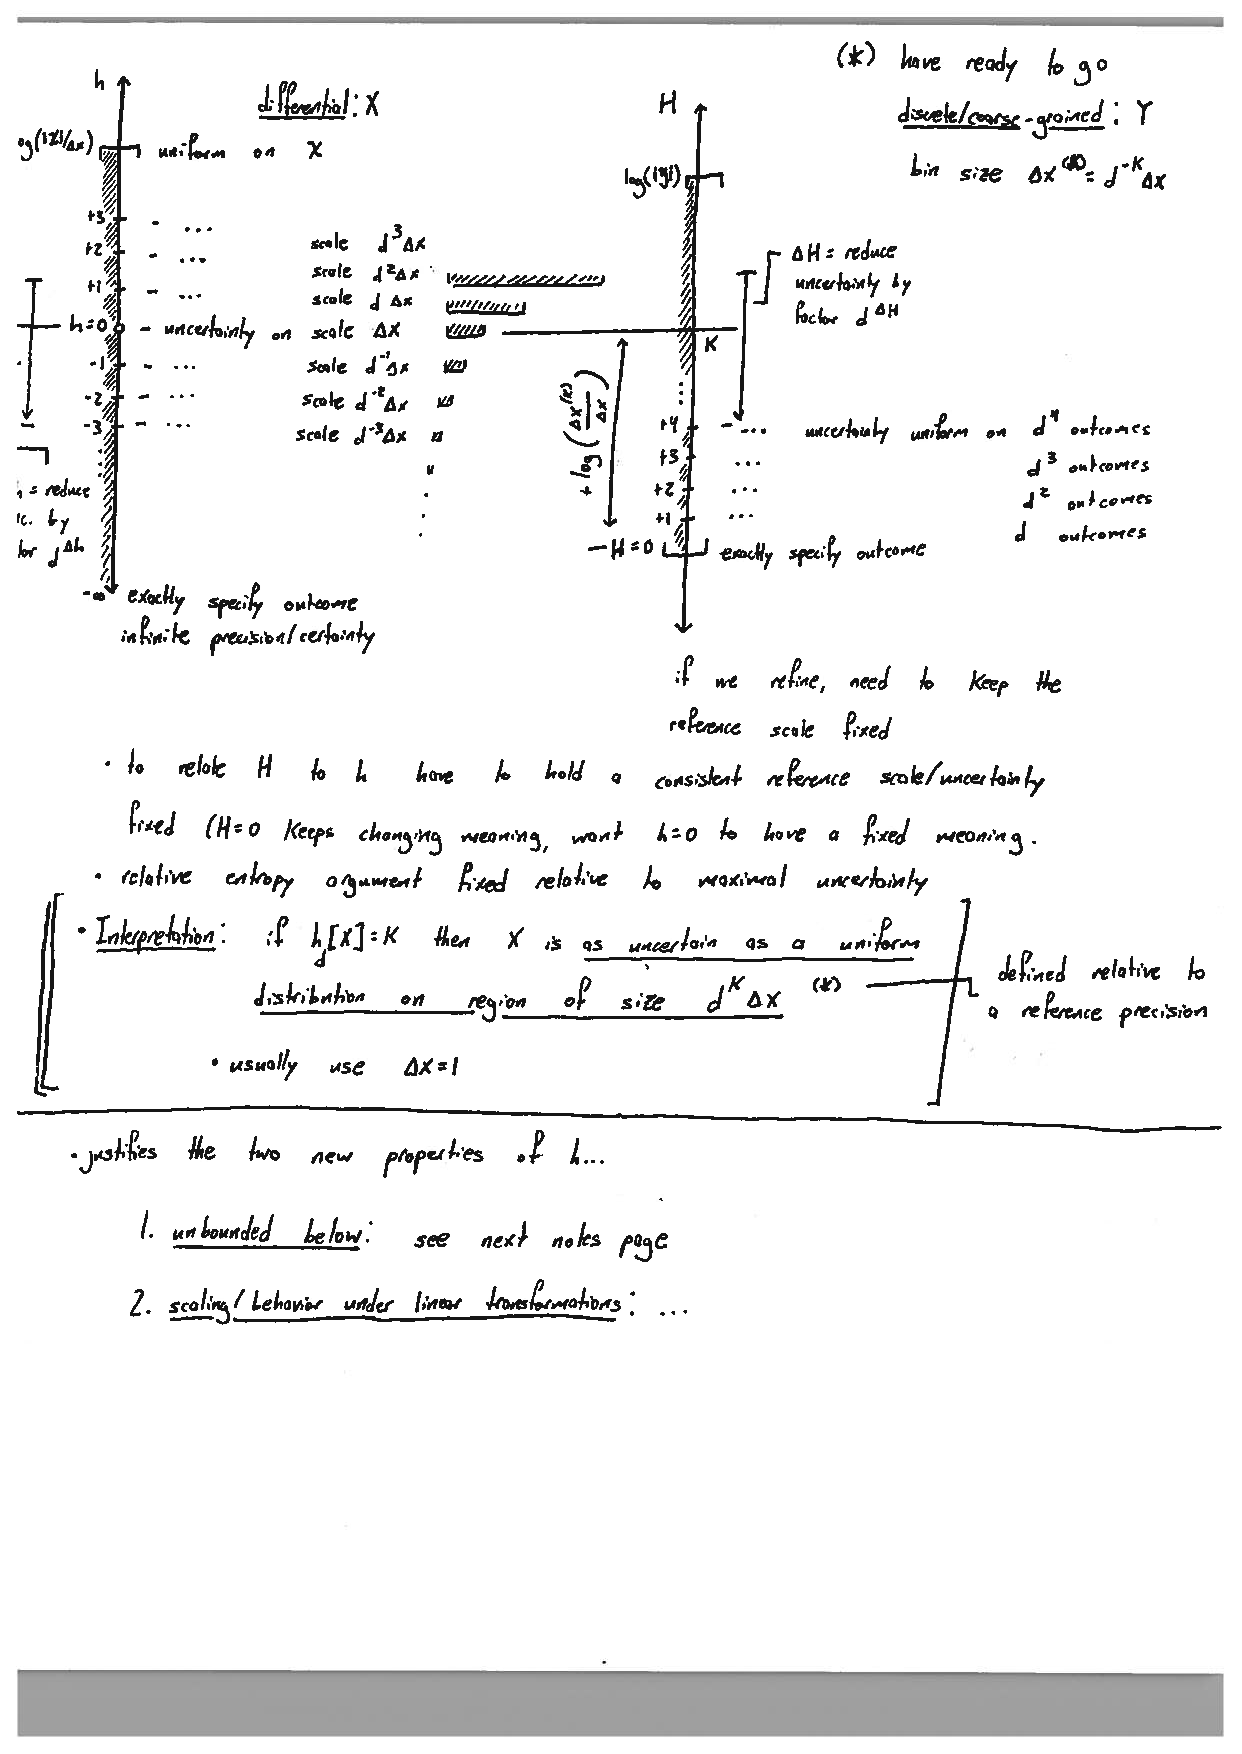
\includepdf[scale=1]{img/Differential_vs_Discrete_schematic.pdf}

% \begin{flalign*}

% \text{Negative relative entropy means we are more certain than our reference scale.}

% \text{If our relative entropy is } -\infty \text{ then we are infinitely more certain than our reference scale (we have exactly specified outcome to infinite precision).}
% \end{flalign*}

\hrulefill

\subsection{Properties of Differential Entropy}
Properties of Differential Entropy that are not shared by discrete entropy:
\begin{enumerate}
    \item Unbounded below: For \( X \sim p \), \( X \in \mathcal{X} \), and \( |\mathcal{X}| \), let \( p = \text{Uni}(|S|) \), then \( h_d[X] = \log_d(|S|) \to -\infty \) as \( |S| \to 0 \).
    \item Extrinsic: We have a reference ground.
\end{enumerate}
Consider transformations \( T: Y = T(X) \), for invertible \( T \).
\begin{itemize}
    \item Example 1: \( T(x) = ax + b \), then \( h[Y] = h[X] + \log(|a|) \).
    \item Example 2: For \( x \in \mathbb{R}^n \), \( T(X) = Ax + b \), \( A \in \mathbb{R}^{n \times n} \), invertible, then we get the change of density formula.
\end{itemize}

\subsection{Gaussian Distribution in Signal Processing}
Now we look at one of the most common distributions in Signal Processing, Real-world applications, etc:
\( X \sim \mathcal{N}(\mu, \Sigma) \), what is \( h[X] \)?
\( X = T(y) \), \( y \sim \mathcal{N}(0, I) \) where \( X = AY + b \) for positive definite \( \Sigma \) such that \( \Sigma^{-1} \) and hence \( A^{-1} \) exists. Let \( b = \mu \), \( \Sigma = AA^T \) as \( \text{Cov}[X] = \text{Cov}[AY] \). If we realize that \( \det(\Sigma^{0.5}) = \det(\Sigma)^{0.5} \) and:
\[ h[Y] = -\mathbb{E}_Y[\log(f_Y(y))] = -\mathbb{E}_Y[\log((2\pi)^{-n/2} \exp(-\frac{1}{2}\sum_{j=1}^n y_j^2))] 
= -\mathbb{E}_Y[-\frac{n}{2} \log(2\pi) - \underbrace{E[Y_j^2]}_1] 
= \frac{n}{2} \log(2\pi e).
\]
Then we can simplify:
\[ h[X] = \frac{1}{2} \log(\det(\Sigma)) + \frac{n}{2} \log(2\pi e). \]
where
$$
h[X] = 1/2 \underbrace{\log(\det(\Sigma))}_{\text{Cov scaling extrinsic dimension}} + \underbrace{n/2}_{\text{dimension}} \underbrace{\log(2\pi e)}_{\text{Gaussian}}.
$$

    \section{Thursday, February 22nd}
\subsection{Time-Frequency Duality}
Draw $\{\hat{X}_j\}\sim f_X,\quad\Xhat\in\cXhat$
\begin{shaded}
Imagine you have a set of basis functions, $\{b_j(t)\}_{j=1}^{n\to\infty}$, \\
then draw a set of coeff.'s $\{\hat{X}_j\}_{j=1}^{n\to\infty}$.\\
Set: $X(t)=\sum_{j=1}^{n}\hat{X}_j b_j(t)$.
\end{shaded}
\begin{figure}[H]
    \centering
    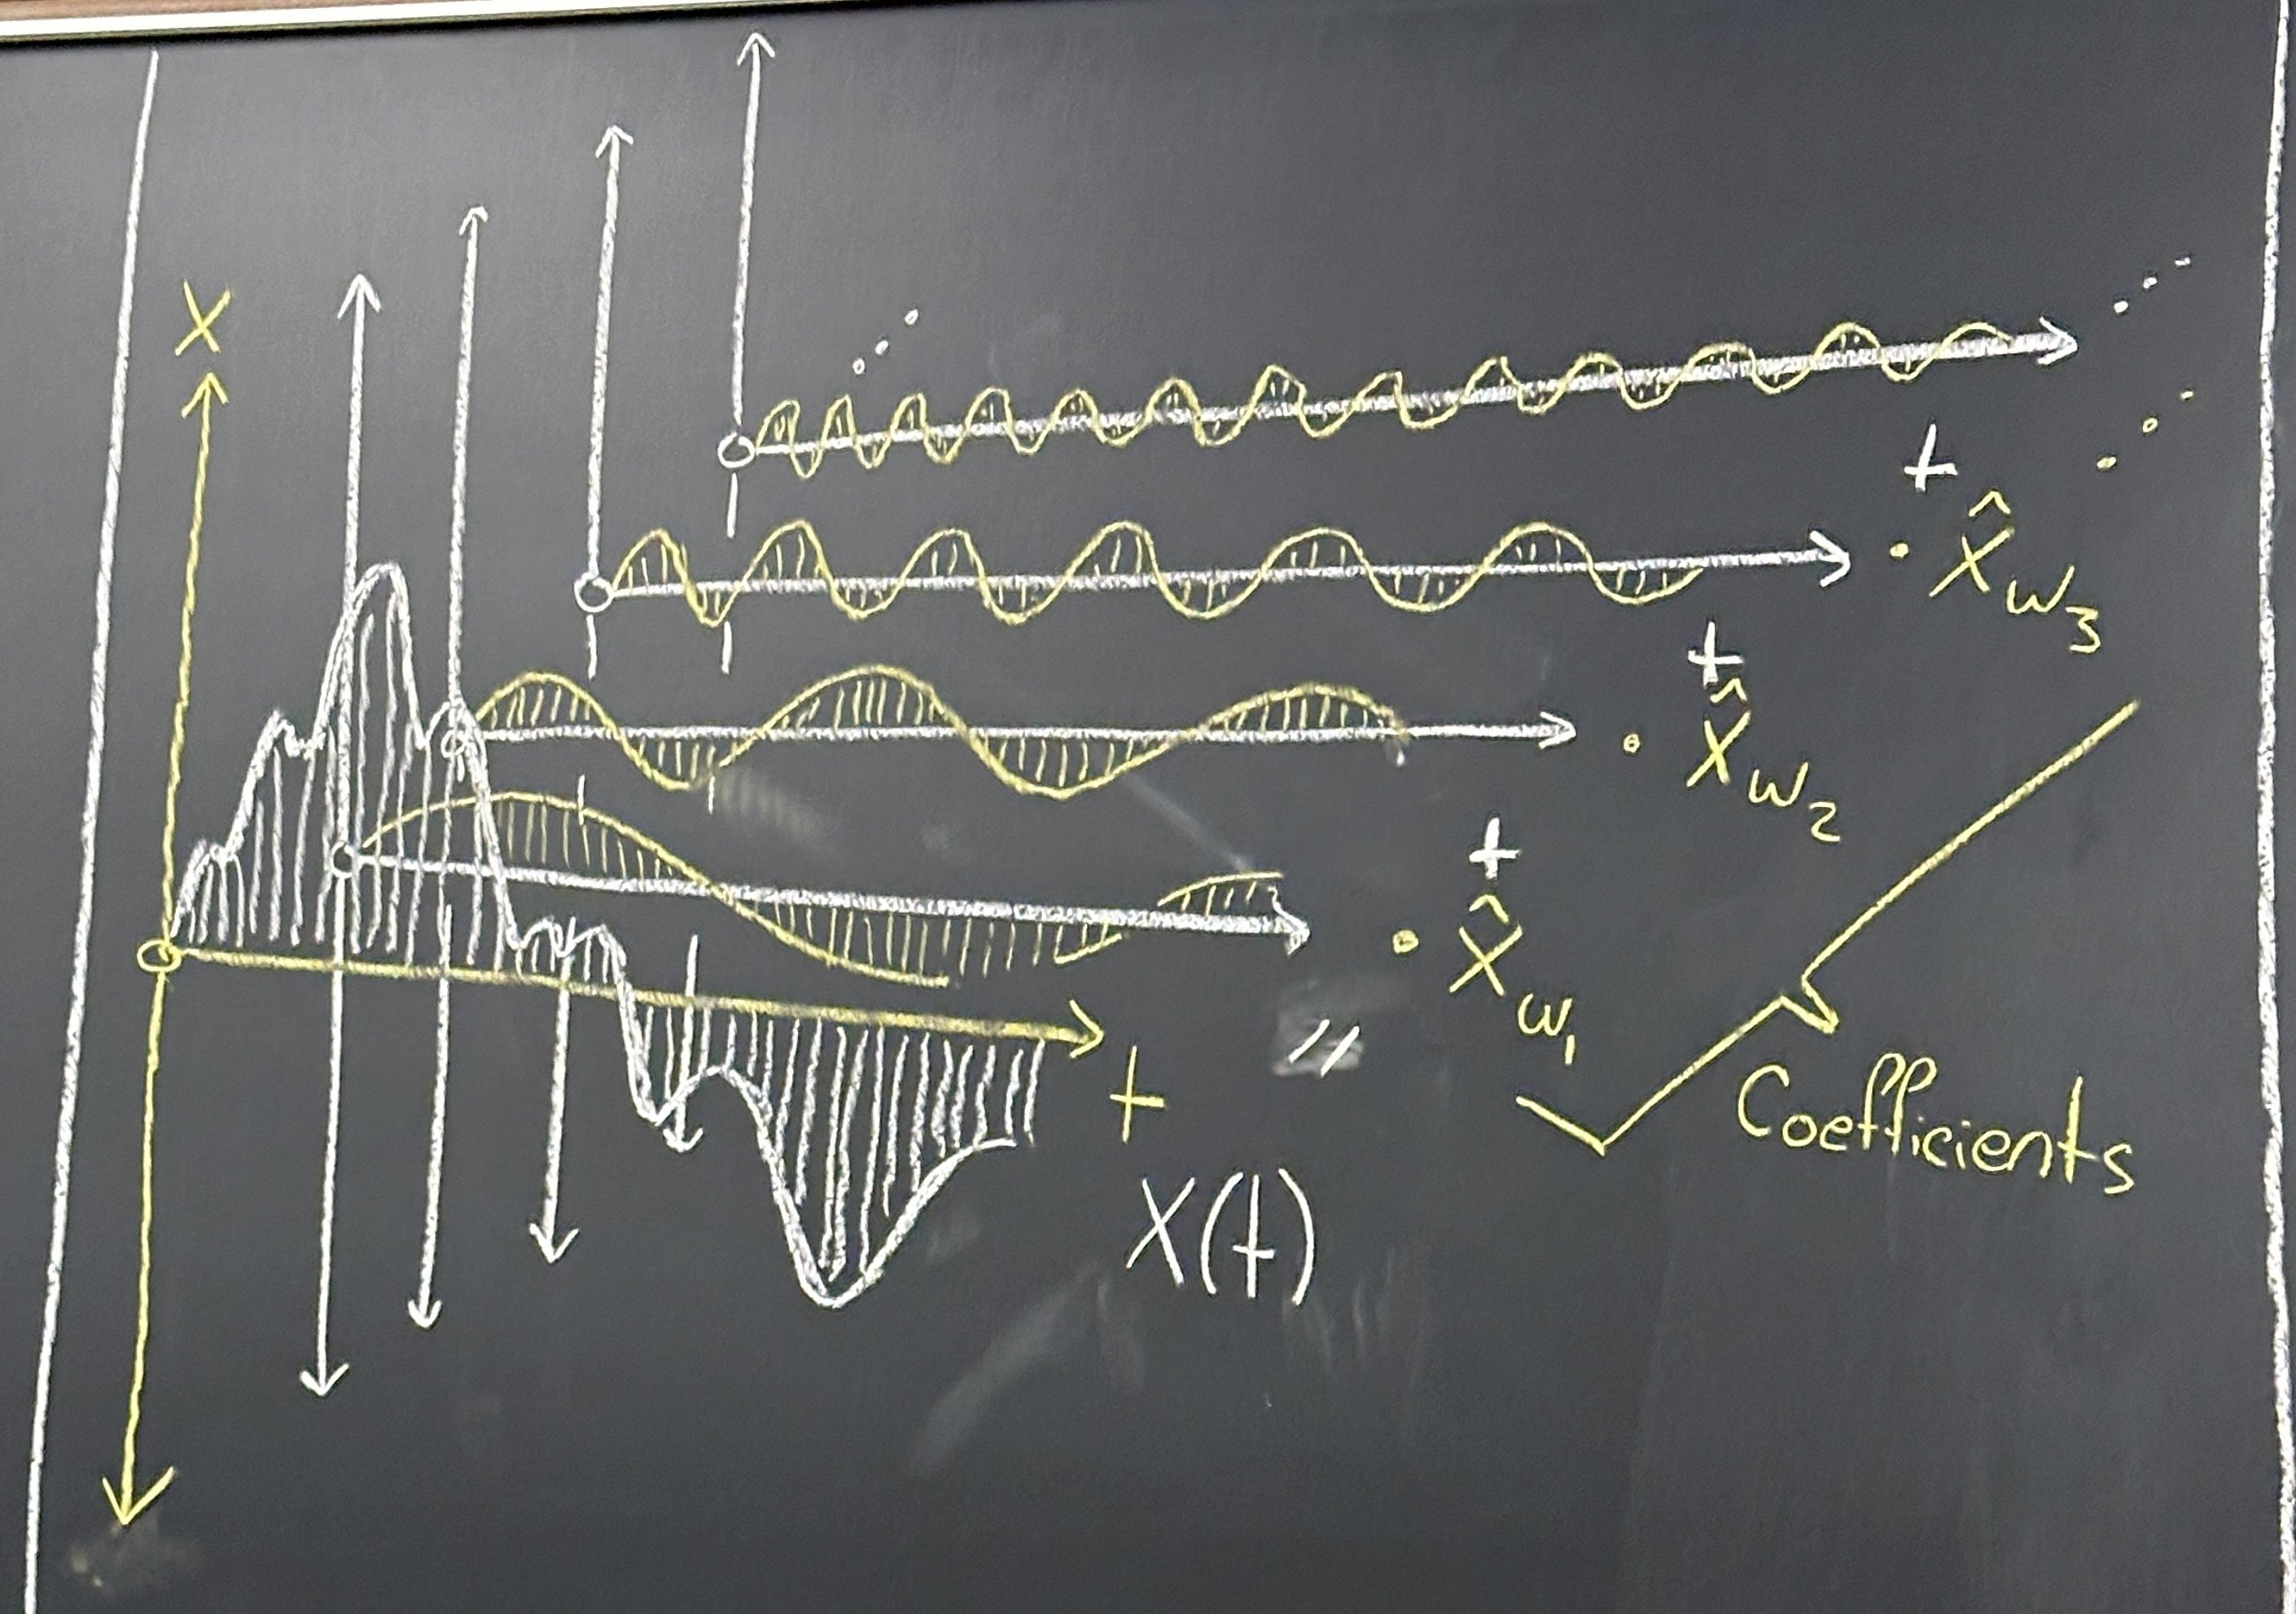
\includegraphics[scale=0.13]{lectures/wk6/img/time-freq.jpeg}
    % \caption{Caption}
    % \label{fig:enter-label}
\end{figure}

\begin{important}
Fourier transforms lose temporal resolution.
\end{important}

\subsection{Stochastic Processes}
\begin{defn}{Stochastic Process}
is a random function $X(t)$.
\end{defn}

Usually you have a SDE (\href{https://en.wikipedia.org/wiki/Stochastic_differential_equation}{Stochastic differential equation}) or a Markov process which is a random operation run conditionally fwd in time.

Here we are generating it all at once by generating a set of coeff.'s. -- this gives some curve thoroughout space.


\subsubsection{Gaussian Processes}
If we draw the set of coeff.'s to be MVG: draw $\Xhat\sim\cN$.
\begin{defn}{Gaussian Process}
$X(t)$ is a Gaussian Process if: \\
for any set of samples $\{t_j\}_{j=1}^n$\\
the r.v. $\vX=\begin{bmatrix}
    X(t_1), X(t_2), \ldots, X(t_n)
\end{bmatrix}, X_j = X(t_j)$ is drawn jointly from a MVG.
\end{defn}


It is a reasonable class of functions to be working with since it is:
\begin{enumerate}
    \item Tractable
    \item Moderately General. Note that it is not completely general, but it is one of the most simple models that gives us this level of generality.
\end{enumerate}

A MVG is uniquely specified by its mean vector 
($\mu(t)=\E[X(t)]$) 
and its covariance matrix 
$$\Sigma=K(t, s)=\Cov(X(t), X(s))=K(s, t)\st {X}\sim\cN\left(\begin{bmatrix}
 \mu(t_1) \\ \mu(t_2) \\ \vdots \\ \mu(t_n)
\end{bmatrix}, \begin{bmatrix}
 K(t_1, t_1) & K(t_2, t_2) & \cdots \\ 
 K(t_2, t_1) & K(t_2, t_2) &  \\ 
 \vdots &  & \ddots \\ 
\end{bmatrix}\right)
$$

\begin{align*}
& K(t, s)=\operatorname{Cov}[X(t), X(s)]=\sum_{j, j=1}^n E\left[\left(\hat{x}_i-\hat{\mu}_i\right)\left(\hat{x}_j-\hat{\mu}_j\right)\right] b_i(t) b_j(s)=\sum_{i j=1}^n\left[\hat{\sum}\right]_j b_i(t) b_j(s) \\
& \text { mean } \mu(t)=\mathbb{E}[X(t)] \\
& =\left[b_1(t), \ldots b_n(t)\right] \hat{\varepsilon}\begin{bmatrix}
b(s) \\
\vdots \\
b_n(s)
\end{bmatrix}=\vec{b}(t)^{\top} \hat{\dot{E}} \vec{b}(s) \\
&
\end{align*}

Suppose $\hat{x}_i \ind \hat{x}, \forall i \neq j$:\\
$
\hat{\Sigma}=\begin{bmatrix}
\hat{\sigma}_1^2 & & & \\
& \hat{\sigma}_2^2 & & \\
& & \ddots & \\
& & & \hat{\sigma}_n^2
\end{bmatrix}
$, 
then: 
$K(t, s)=\sum_{j=1}^n \hat{\sigma}^2, b_j(t) b_j(s).$

\subsection{Mercer's Theorem}
For most reasonably defined $K, \exists$ an expansion of the kind above for some, $\{b\}_{j=1}^{n \rightarrow \infty}$.

\subsection{Bochner's Theorem}
If $X(t) \sim X(t+s)$ for any $s$ then $b_j$'s are Fourier Modes.

\subsection{Shannon-Nyquist Theorem}
If $X(t)$ does not contain any frequencies higher than some band limit $B$, then $X(t)$ can be fully recovered (all the information in $X(t)$ are captured) by finitely many samples sufficiently close, $\Delta t < \frac1{2B}$.

\subsection{Entropy/Information:}
\begin{enumerate}
    \item In terms of samples, 
    \item In terms of the coeff. $\Xhat$
\end{enumerate}

$\cF\inv: 1\mapsto 2$ and $\cF: 2\mapsto 1$. Furthermore Shannon gives us this $\cF$.

\begin{shaded}
Question: How do I know that I can sample from fractional timesteps (finer samples).
\end{shaded}
This is a common question in compression, assume you are trying to store a song

Answer: Naively we could just store everything.

Well, $\vX=\begin{bmatrix}
    X(t_1), \ldots, X(t_n)
\end{bmatrix}$.\\
$\vX\sim\cN(\vmu, K)$\\
$h[\vX]=\frac12\log((2\pi e)^n |K|)=\frac12\log(|\det(K)|) +\frac{n}2\log(2\pi e)$\\
Suppose: 
\begin{flalign*}
I(\vX, \vX) &= h(\vX) - h(\vXp\mid \vX) \\
    &= h(\vX) + h(\vX) - h(\vXp, \vX)
    &&[\text{Chain Rule}]
    \\
    &= \frac12\left[\log(|K_{\Xp\Xp}|) 
    + \log(|K_{XX}|) - \log(|\begin{bmatrix}
        K_{\Xp\Xp} & K_{\Xp X}
        \\
        K_{X\Xp} K_{XX}
    \end{bmatrix}|)\right]
    \\
    &=-\frac{1}{2} \log \left(1-\rho^2\right)
\end{flalign*}


% diagram of my(t)
Smoothness of underlying GP related to MI on refined sampling.

\hrulefill

\begin{itemize}
    \item $X\sim\cN(\mu, \Sigma)$, 2D.
    \item If $\Sigma$ has SVD: $\Sigma=U \begin{bmatrix}
        \sigma_1^2 & 0 \\
        0 & \sigma_2^2 \\
    \end{bmatrix} U^\top$.
\end{itemize}

    
%     \section{Tuesday, February 27th}
%     \subsection{Is Information Intrinsic?}
%     \begin{minipage}{\textwidth}
%     \includepdf[scale=0.7]{./lectures/wk7/isInformationIntrinsic.pdf}
%     \end{minipage}
%     \includepdf[pages=2-]{./lectures/wk7/isInformationIntrinsic.pdf}

% % \newpage
%     \subsection{Gaussian Examples: Mutual Information for Random Vector}
%     \begin{minipage}{\textwidth}
%     \includepdf[scale=0.8]{./lectures/wk7/GaussianExamples.pdf}
%     \end{minipage}
%     \includepdf[pages=2-]{./lectures/wk7/GaussianExamples.pdf}

%     \section{Thursday, February 29th}
%     \subsection{Information Inequalities II: Data Processing and Fano}
%     \begin{minipage}{\textwidth}
%     \includepdf[scale=0.7]{./lectures/wk7/InformationInequalitiesII.pdf}
%     \end{minipage}
%     \includepdf[pages=2-]{./lectures/wk7/InformationInequalitiesII.pdf}

%     \subsection{What is Relative Entropy (KL)? Part 1: Review}
%     \begin{minipage}{\textwidth}
%     \includepdf[scale=0.7]{./lectures/wk7/RelativeEntropy_Part1.pdf}
%     \end{minipage}
%     \includepdf[pages=2-]{./lectures/wk7/RelativeEntropy_Part1.pdf}

%     \subsection{What is Relative Entropy (KL)? Part 2: Statistical Interpretation}
%     \begin{minipage}{\textwidth}
%     \includepdf[scale=0.7]{./lectures/wk7/RelativeEntropy_Part2.pdf}
%     \end{minipage}
%     \includepdf[pages=2-]{./lectures/wk7/RelativeEntropy_Part2.pdf}

    
    
    \section{Tuesday, March 5th}
\subsection{Logistics}
Proposal is no longer due this Thursday, now due next Tuesday. 

A lot of students are doing the discussion only just before classes. At least once reply must be posted before (midnight on Saturday).

\subsection{Goals for the week:}
\begin{enumerate}
    \item Week 7 (Information) Review
    \item Information Geometry
    \begin{itemize}
        \item Example on Maximum Geometry
    \end{itemize}
\end{enumerate}
\subsubsection{Challenge for the week:}
\begin{important}
\textbf{Challenge:} Use Maximum Geometry to prove the \textit{Central Limit Theorem}.
\end{important}

\subsection{Review of last week:}
If we have $\{X_i\}_{i=1}^n\simiid p$ where $p = p_0$ or $p_1$.

\begin{align*}
S &= s(X_1, \ldots, X_n) = \log\left(\frac{\P[X_1, \ldots, X_n \mid p_1]}{\P[X_1, \ldots, X_n \mid p_0]}\right)
\end{align*}
\begin{important}
Note for quiz 4: The order for entries in a KL divergence do matter. You will be tested on this order. The one that goes first is the one you are drawing from:
\begin{equation}
    \E_{X\sim p_1}[S] = n D(p_1||p_0)
\end{equation}

\begin{equation}
    \E_{X\sim p_0}[S] = -n D(p_0||p_1)
\end{equation}
\end{important}
\begin{center}
    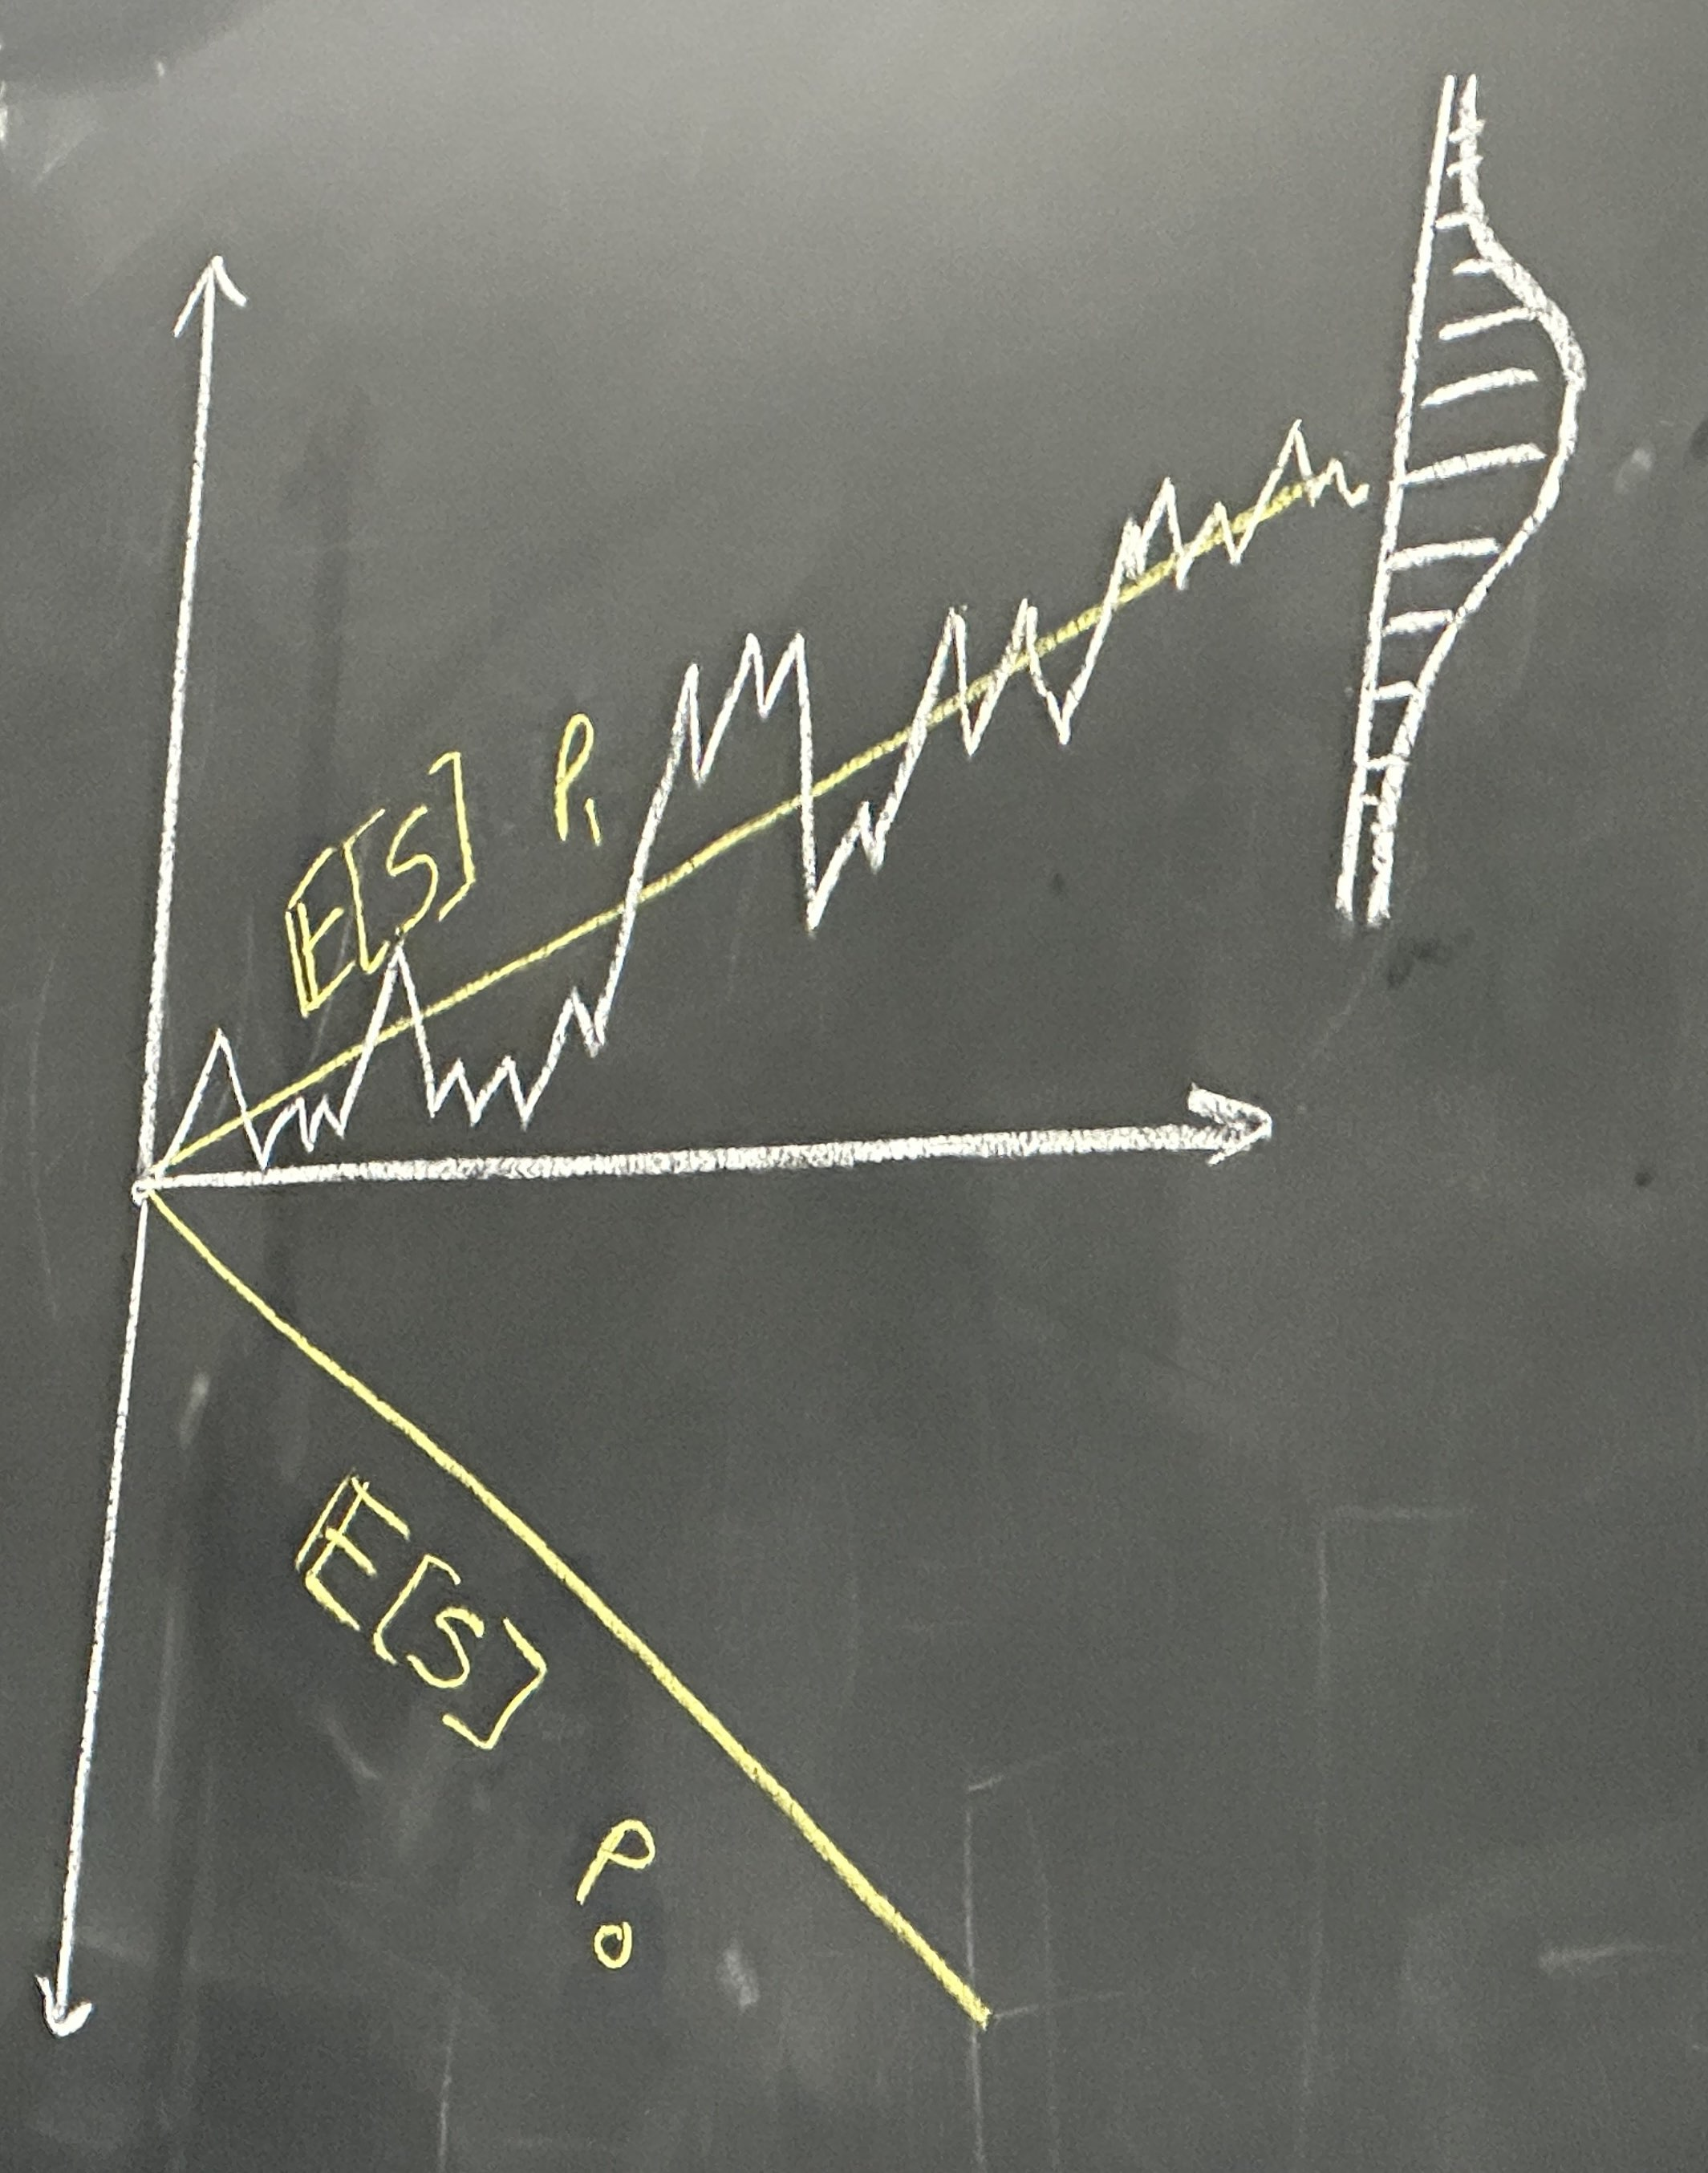
\includegraphics[scale=0.1]{lectures/wk8/img/img1.jpeg}
\end{center}
Note that $D$ controls the slope: increasing it (a change in $D$) tells you that it will be more clearly distinguishable.

Vertical distribution = background sampling distribution.

\subsection{Brownian Bridge}
\begin{center}
    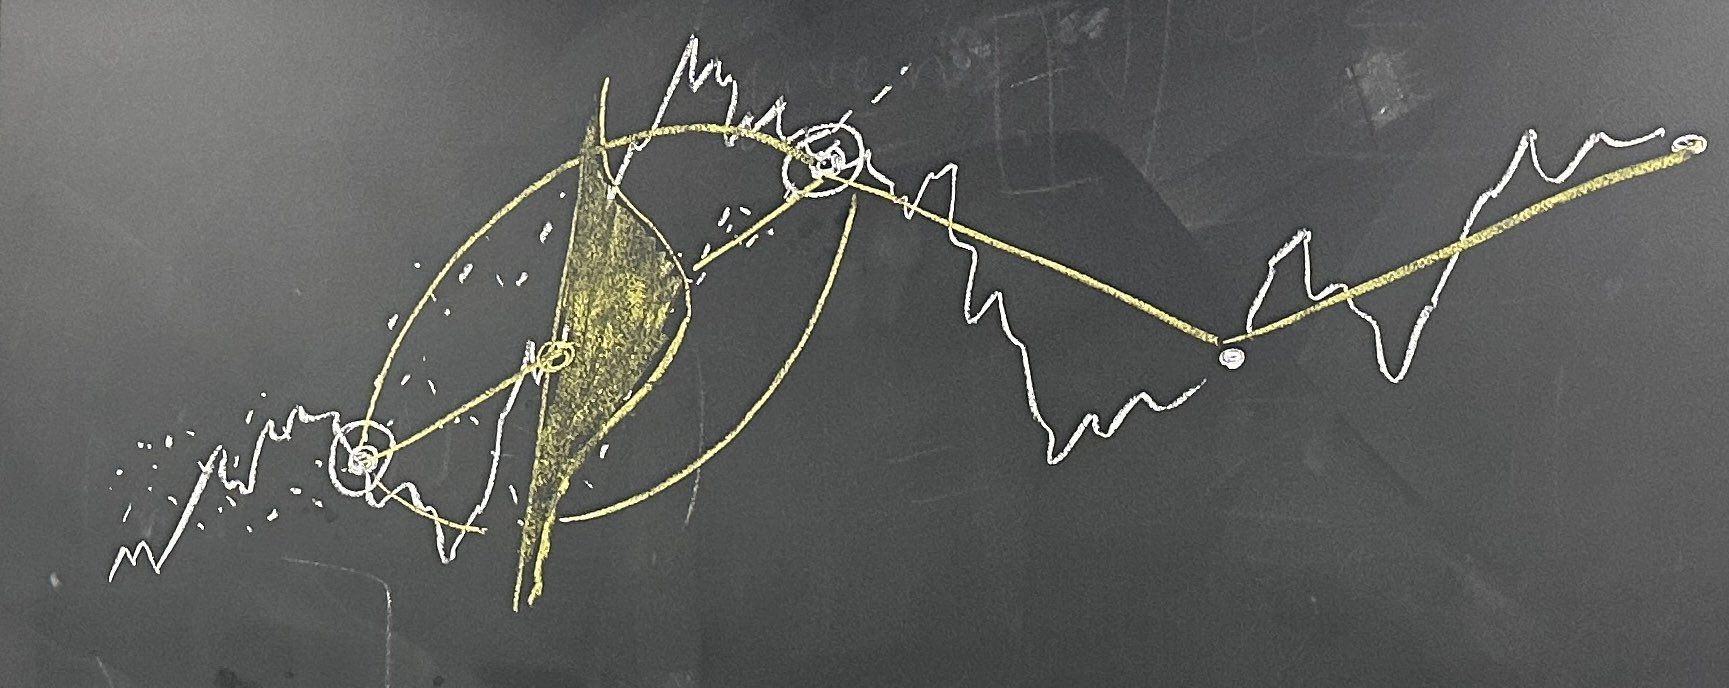
\includegraphics[scale=0.25]{lectures/wk8/img/img2.jpeg}
\end{center}

\subsection{Problem:}
\begin{enumerate}
    \item Target distribution $p_0$
    \item Chosen divergence $D$
    \item Variational family of distribution $\cP = \{\text{ set of dist. }\}$
    \begin{enumerate}
        \item[(i)] \underline{implicit}: via constraints
        \item[(i)] \underline{explicit}: via parameterized model $\{P_\Theta\}_{\text{all }\Theta}$
    \end{enumerate}
\end{enumerate}
Goal: minimize $D(p||p_0), D(p_0||p)$ given: $p\in\cP$. 

The class of F-divergences is convex, so it can be formulated as a convex optimization problem in most cases. 

\subsubsection{Variational Calculus}
Note that you will need to use variational calculus instead of regular calculus in some choices of divergence (see the book for examples on this).

\subsubsection{Fréchet derivatives}
The derivative defined on normed spaces.

\subsubsection{3D Probability Simplex}
Within this set is our target -- note that any point in the set is a distribution. 

\begin{center}
    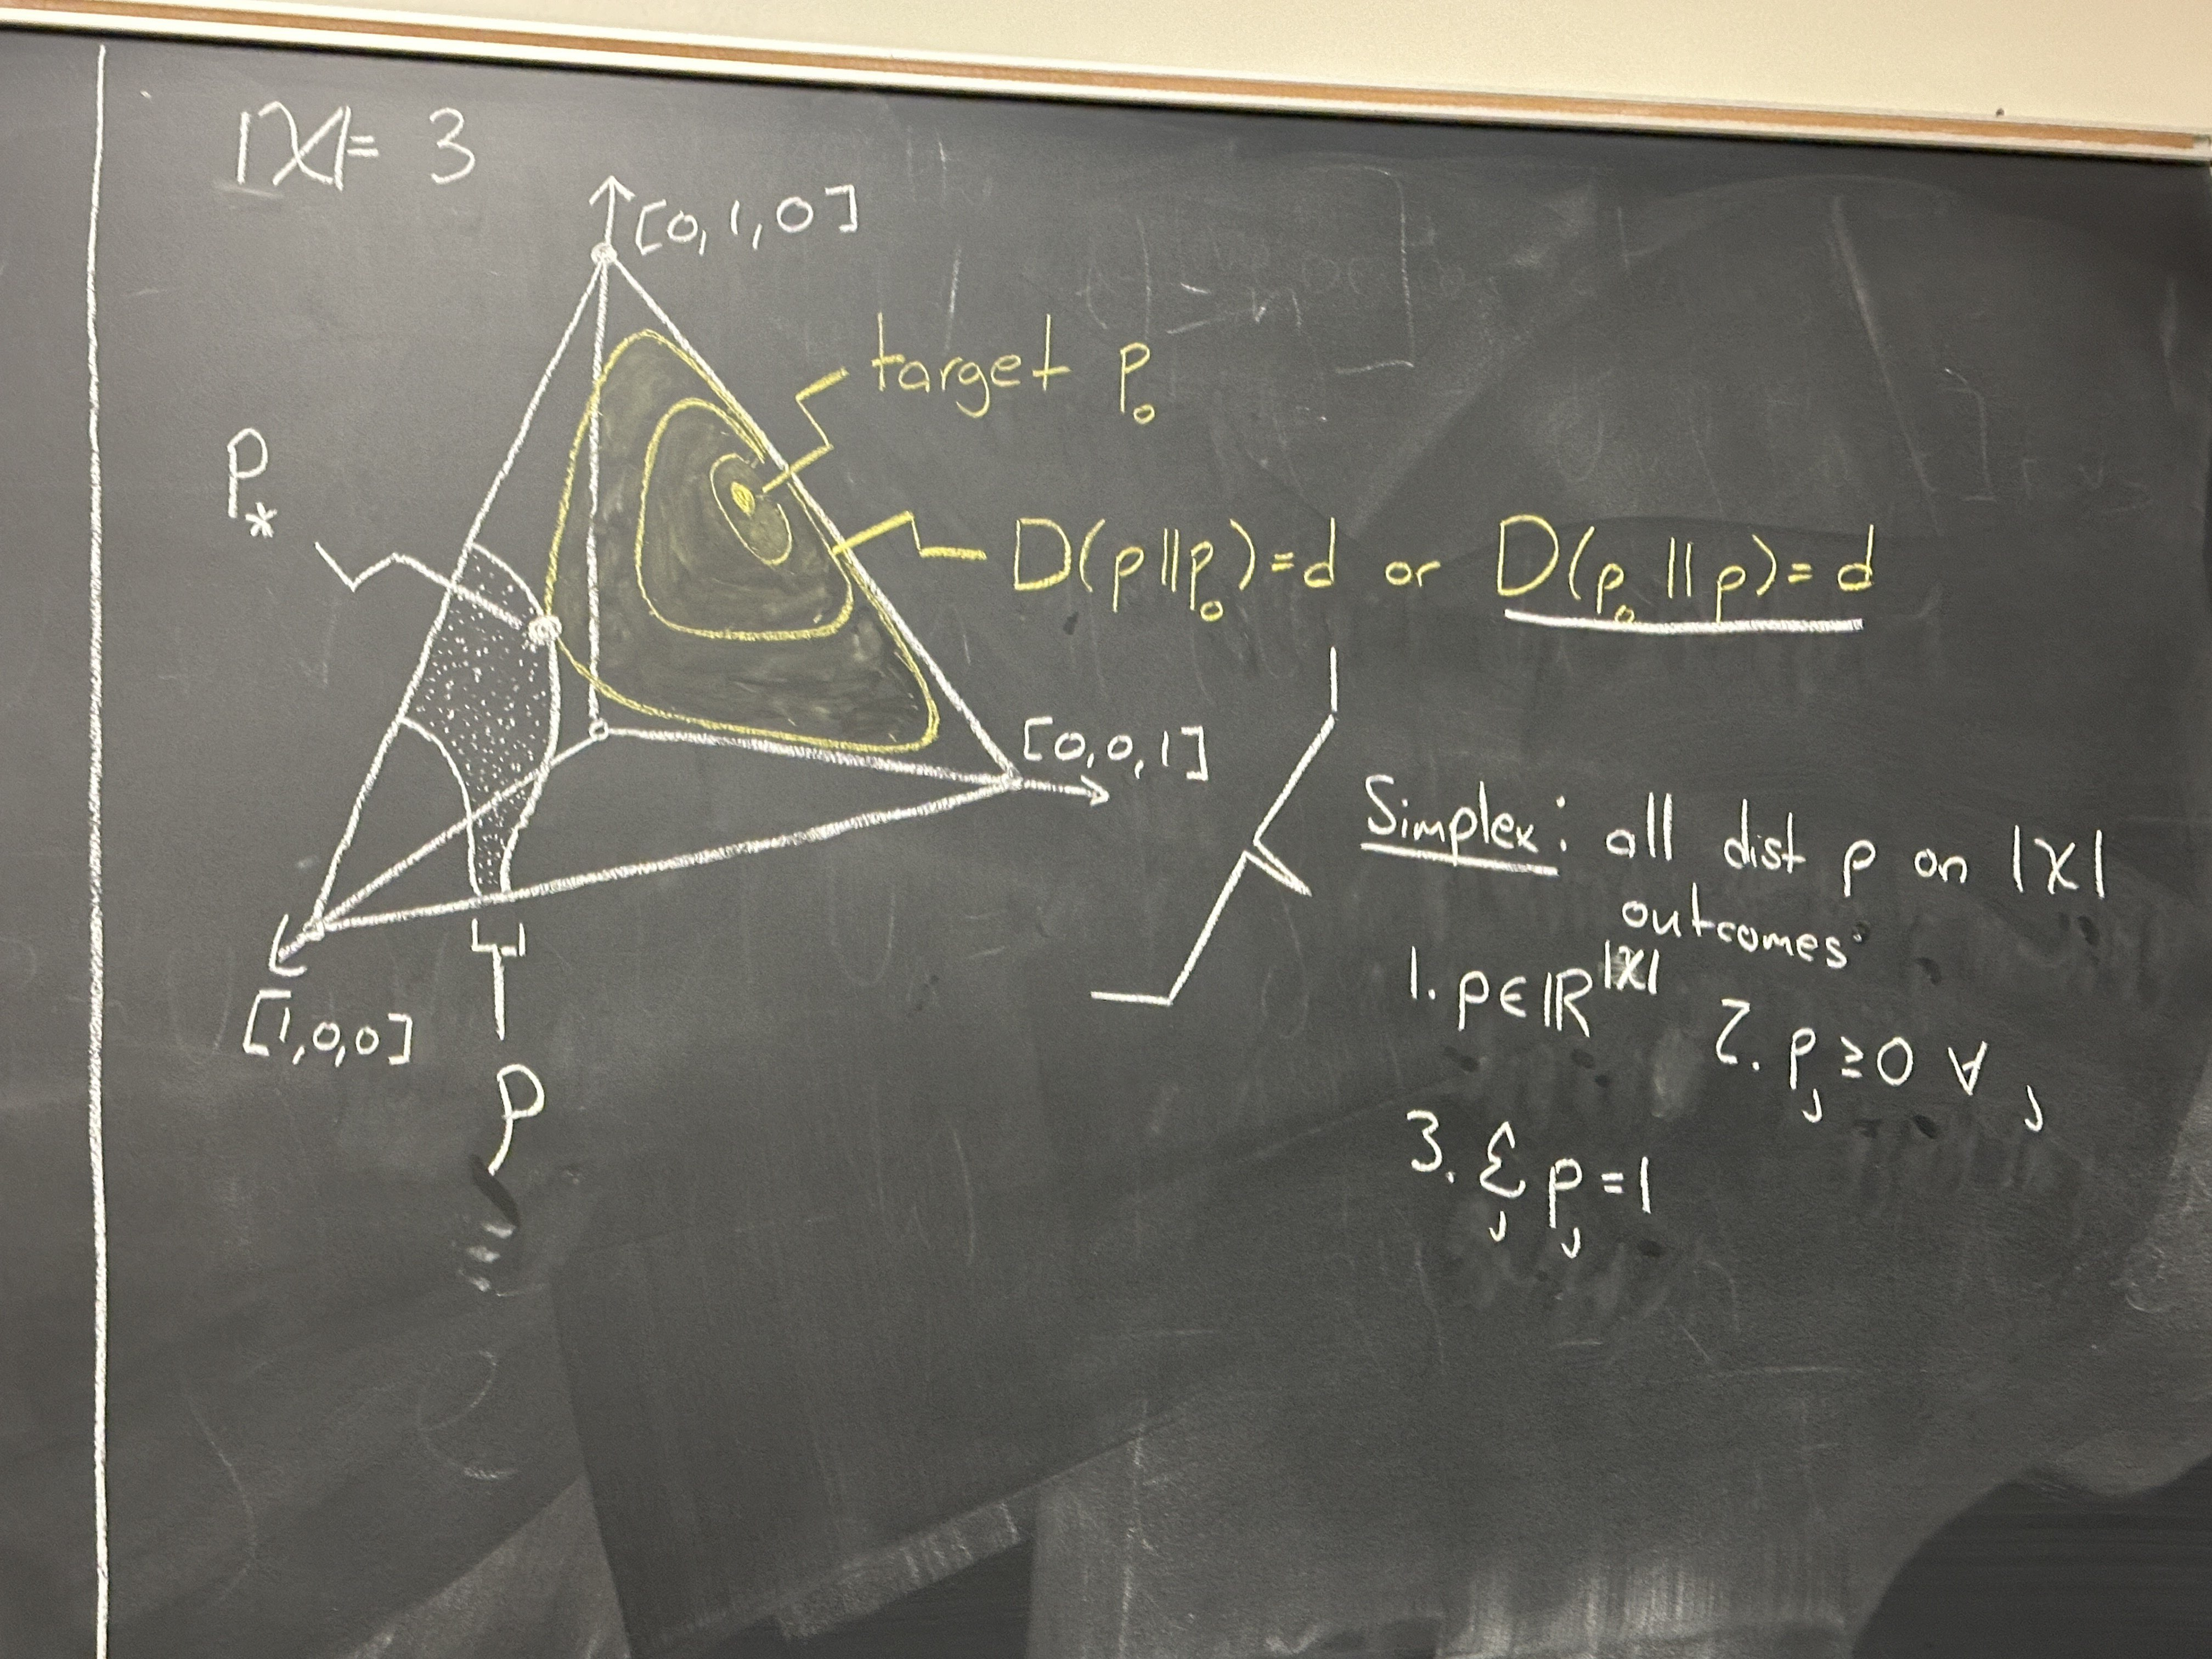
\includegraphics[scale=0.1]{lectures/wk8/img/img3.jpeg}
\end{center}

We look at the level sets that have distance $d$ away from our target $p_0$.

\subsection{Convergence in distribution on a Weak Topology}
$\underbrace{D_{KL}(p_0 || p)}_{\to0} \geq\frac1{\ln2} \underbrace{\text{TV}(p, p_0)^2}_{0} \to p \Rightarrow p_0$ which is weak convergence, 
where $\text{TV}$ is the total variation distance.

\subsection{Maximum Entropy: A constrained optimization problem}
$X\sim p$, where $p$ is unknown, but we do ``know'' some moments.

We implicitly define $\cP$ as follows:
\subsubsection{Equality:}
\underline{Equality} $\cF_i[p] = \E_{X\sim p}[f_i(x)]=\{\alpha_i\}_{i=1}^n$.

Examples:
\begin{align*}
      \E[X],& f(x) = x \\
    \E[X^2],& f(x) = x^2 \\
    &\vdots
\end{align*}


\subsubsection{Inequality:}
\underline{Inequality} $\cG_i[p] = \E_{X\sim p}[g_j(x)]\geq\{\alpha_j\}_{j=1}^m$.

\subsubsection{Goal}
We want to $\max H(p), \quad p\in\cP\implies p_\ast = 
\displaystyle\argmax_{p\in\cP} \{H(p)\}$.

\subsection{Question:}
\begin{equation}
    \max_{p\in\cP} \{H(p)\} \iff \min_{p\in\cP} \{D(? || ?)\}?
\end{equation}
\begin{important}
Quiz: You want to relate the above to the KL divergence of a uniform distribution.
\end{important}
\begin{align*}
    H(p) &= -\E_{x\sim p}[\log(p(x))]
    = -\E_{x\sim p}[\log(\frac{p(x)}{1/|\cX|} \cdot \frac1{|\cX|})]
    \\
    &= -\E_{x\sim p}[\log(\frac{p(x)}{1/|\cX|})] + \E_{x\sim p}[\log(|\cX|)] \\
    &= -D(p||U[\cX]) + H[U[\cX]] \\
H(p) &= H(U(\cX)) - D(p || U[\cX]) \\
\implies &\max_{p\in\cP} \{H(p)\} \iff \underbrace{\min_{p\in\cP} \{D(p || U[\cX])\}}_{\text{Occam's Razor for $\max H$}}
\end{align*}

\subsection{Karush-Kuhn-Tucker (KKT) Conditions:}
For Convex differentiable functions, how do we find sufficeient and necessary stationary conditions? How do we generalize Lagrange multipliers for when we have inequality constraints?

Given $\cP = \left\{p\st \underbrace{\{\cF_i[p]=\alpha_i\}_{i=1}^n}_{\text{equality}}, \underbrace{\{\cG_j[p]=\alpha_j\}_{j=1}^n}_{\text{inequality}} \right\}$

For an objective: $H(p)$
\begin{enumerate}
    \item $\left.-\nabla_p H(p) + \sum_{i=1}^n \lambda_i \nabla_p \cF(p) + \sum_{j=1}^n \mu_j \nabla_p \cG(p)\right|_{p=p^\ast}=0$
    \item $p^\ast\in\cP$
    \item $\mu_j\geq0\quad\forall j$
    \item if $G_j[p] \gneq \beta_j$ then $\mu_j=0$.
\end{enumerate}

\underline{moment:} $\cF[p] = \E_{x\sim p}[f(x)] = \sum_{\text{all $x$}} p(x) f(x)$

We are restricted to a polytope, that is a subset of a face on the simplex. 

The constraints listed above are called:

0th order optimality condition: $\forall x, p(x)\geq 0\mapsto p(x')=\begin{cases}
    0 \quad \text{ if } x'\ne x
    \\
    1 \quad \text{ if } x' = x
\end{cases}$.
\begin{enumerate}
    \item Stationarity (first order optimality condition): 
    $\sum_x p(x)=1
    \mapsto\partial_{p(x)} \sum_{x'} p(x')=1$.
    \item Feasibility (Primal), it has to live inside the set of possible distributions.
    \item Feasibility (Dual): Non-negativity, your gradient should be pointed out (not into) your set.
    \item Complementary Slackness (Active/Inactive): $\lambda_i^* h_i\left(x^*\right)=0, \forall i\quad \iff \sum()$.
\end{enumerate}

The gradient of our objective function must be parallel to the gradient of our constraints.

\subsection{Taking Derivatives:}
\begin{align*}
H(p)
&\mapsto -\partial_{p(x)} \E_{x\sim p}[\log(p(x))]  \\
&= -\partial_{p(x)} \sum_{x'}[p(x') \log(p(x'))]  \\
&= -\partial_{p(x)} [p(x) \log(p(x))]  \\
&= -\log(p(x)) - 1 \\
&= -(\log(p(x)) + 1)
\end{align*}





If the normal distribution maximizes entropy for a known mean and variance, since it is capped above by a gaussian's    .

Convergence in KL is convergence in distribution.

    \section{Thursday, March 7th}
\subsection{Method of Types}
\begin{itemize}
    \item $X\in \cX, |\cX|<\infty$
    \item $X^{(n)} = \{X_i\}_{i=1}^n, X\simiid p_0$
\end{itemize}

\subsection{Empirical Distribution}
$X^{n} = x^{n}$ is 
\begin{itemize}
    \item Draw $J \sim \Uniform[1, n]$
    \item Y = $X_j$
\end{itemize}
$P(Y = y) = \frac{\# \text{ of } \st x_j = y}{n}$

\begin{equation}
    \cP^{(n)} = \{\text{frequency of the outcome } y \text{ among } \{x_{i}\}_{i=1}^n\}
\end{equation}

\subsection{Type}
\textbf{Definition:} A type $P$ is a probability distribution on $|\cX|$ outcomes w/ rational prob., denominator is $n$.

\subsubsection{Type Class}
The \underline{type-class} $T(P)$, 
\begin{equation}
    T(P) = \{ x^{(n)} \text{ s.t. empirical dist } P_{X^{(n}}(\cdot)=P\}
\end{equation}
\begin{enumerate}
    \item The size of $T(P)$ is combinatorial, \# distinct rearrangements of $x^{(n)}$ of $T(P_{x^{(n)}})$
    \item all draws $x^{(n)}\in T(P)$ are equiprobable
\end{enumerate}

Looking at draws (type class) of length 6, when the event can have 3 outcomes, we view them as points in the simplex (space of possible distributions) as opposed to bar charts.

\subsection{Theorem 11.1.1}
As stated in T\&C, 
The number of types with denominator $n$ is bounded by
$$
\left|\mathcal{P}_n\right| \leq(n+1)^{|\mathcal{X}|}.
$$

\subsection{Theorem 11.1.2}
As stated in T\&C, If $X_1, X_2, \ldots, X_n$ are drawn i.i.d. according to $Q(x)$, the probability of $x^n$ depends only on its type and is given by
$$
Q^n\left(x^n\right)=2^{-n\left(H\left(P_x n\right)+D\left(P_x n || Q\right)\right)}.
$$

\subsubsection{Multiplicity vs Fitting to Data Generating Distribution}
Multiplicity: $H_d(P_{x^{(n)}})$.

Fitting to Data Generating Distribution $p_0$: $D_d(P_{x^{(n)}} || p_0)$

\subsection{Theorem 11.1.3: Size of a type class T(P)}
For any type $P \in \mathcal{P}_n$,
$$
\underbrace{\frac{1}{(n+1)^{|\mathcal{X}|}}}_{\text{Polynomial}} d^{n H(P)} \leq|T(P)| \leq d^{n H(P)} .
$$

This goes beyond excess surprise and gives us something to bound any probability distribution by.

\subsection{Theorem 11.1.4: Prob. of a type class T(P)}
For any $P \in \mathcal{P}_n$ and any distribution $Q$, the probability of the type class $T(P)$ under $Q^n$ is $2^{-n D(P \| Q)}$ to first order in the exponent. More precisely,
$$
\frac{1}{(n+1)^{|\mathcal{X}|}} 2^{-n D(P \| Q)} \leq Q^n(T(P)) \leq 2^{-n D(P \| Q)} .
$$

\subsection{Key Equation}
$$
D(P \| Q) \stackrel{\tiny{n\to\infty}}\simeq =-\frac1n \log_d(P(X^{(n)} \in T(P)).
$$
where $\simeq$ means asymptotically equal. This is used in several proofs, including that of CLT.

    \section{Tuesday, March 12th}
\subsection{Logistics}
\begin{itemize}
    \item Project Part 3 due today -- Part 4 will be out this week
    \begin{itemize}
        \item Note you only have finitely many slip days.
    \end{itemize}
    \item Discussion due Thursday
    \item Quiz 4 retake Thurs (9:30am, 1:30pm)
    \item Quiz 5 (on chapter 11) on Thursday
    \begin{itemize}
        \item Note this plays a similar role as Chapter 5 on Entropy, but on Information: Interpreting info in more applied settings. Thus this will be mainly a quiz on statements/theorems.
    \end{itemize}
\end{itemize}

\subsection{Activity Groups:}
We will examine the following 3 so we can determine proper use cases between them. The distinguishability (expectation of the test statistic) of two distributions is its KL Divergence.

\begin{shaded}
    $D(p \| q)$ is \underline{how distinguishable $p$ is from $q$}, where distinguishabililty is how much samples you need asymptotically, s.t. you can separate them (tell which came from which distribution) w.h.p.. 
\end{shaded}

\begin{shaded}
    $I[X; Y]$ is \underline{$D(p_{X, Y}\| p_{X} p_{Y})$}, how distinguishable the true joint is from the product (thus they are a measure of dependence). Note that this even holds for non-linear dependence.
\end{shaded}

Example:
\begin{shaded}
    $H(p)$ is \underline{the compression of a r.v.}.
\end{shaded}

\newpage
\subsubsection{LLN (Thm 11.2.1)}
\begin{shaded}
Theorem 11.2.1 Let $X_1, X_2, \ldots, X_n$ be i.i.d. $\sim P(x)$. Then
$$
\operatorname{Pr}\left\{D\left(P_{x^n}|| P\right)>\epsilon\right\} \leq 2^{-n\left(\epsilon-|\mathcal{X}| \frac{\log (n+1)}{n}\right)},
$$
and consequently, $D\left(P_{x^n} \| P\right) \rightarrow 0$ with probability 1.
\end{shaded}

\begin{Answer}
\textbf{Proof:} The inequality (11.69) was proved in (11.68). Summing over $n$, we find that
$$
\sum_{n=1}^{\infty} \operatorname{Pr}\left\{D\left(P_{x^n} \| P\right)>\epsilon\right\}<\infty
$$
Thus, the expected number of occurrences of the event $\left\{D\left(P_{x^n} \| P\right)>\epsilon\right\}$ for all $n$ is finite, which implies that the actual number of such occurrences is also finite with probability 1 (Borel-Cantelli lemma). Hence $D\left(P_{x^n} \| P\right) \rightarrow 0$ with probability 1.
$\hfill\square$
\end{Answer}

The Empirical Distribution converges i.p. to the true distribution as $n\to\infty$.

The prob. of observing an Empirical Distribution that is far away from the true distribution is vanishing (so we converge i.p.).

Thus w.h.p., $D(p\|q)<\varepsilon$.

Look for $\mathcal{E}(n)\stackrel\to{n\to\infty}0$ s.t. $\P[D(P_{x^n} \| P_0) < \mathcal{E}(n)] \to 1$.

This leads to the fact that we can do estimation with data.

\newpage
\subsubsection{Sanov \& Conditional Limit (Thm 11.4.1, 11.6.2)}
\begin{shaded}
Theorem 11.4.1 (Sanov's theorem) Let $X_1, X_2, \ldots, X_n$ be i.i.d. $\sim Q(x)$. Let $E \subseteq \mathcal{P}$ be a set of probability distributions. Then
$$
Q^n(E)=Q^n\left(E \cap \mathcal{P}_n\right) \leq(n+1)^{|\mathcal{X}|} 2^{-n D\left(P^*|| Q\right)},
$$
where
$$
P^*=\arg \min _{P \in E} D(P \| Q)
$$
is the distribution in $E$ that is closest to $Q$ in relative entropy.
If, in addition, the set $E$ is the closure of its interior, then
$$
\frac{1}{n} \log Q^n(E) \rightarrow-D\left(P^* \| Q\right) .
$$
\end{shaded}

\begin{Answer}
\textbf{Proof:} We first prove the upper bound:
\begin{align*}
Q^n(E) & =\sum_{P \in E \cap \mathcal{P}_n} Q^n(T(P)) \\
& \leq \sum_{P \in E \cap \mathcal{P}_n} 2^{-n D(P \| Q)}
\\
& \leq \sum_{P \in E \cap \mathcal{P}_n} \max _{P \in E \cap \mathcal{P}_n} 2^{-n D(P \| Q)} \\
& =\sum_{P \in E \cap \mathcal{P}_n} 2^{-n \min _{P \in E \cap \mathcal{P}_n} D(P \| Q)} \\
& \leq \sum_{P \in E \cap \mathcal{P}_n} 2^{-n \min _{P \in E} D(P \| Q)} \\
& =\sum_{P \in E \cap \mathcal{P}_n} 2^{-n D\left(P^* \| Q\right)} \\
& \leq(n+1)^{|\mathcal{X}|_2} 2^{-n D\left(P^* \| Q\right)},
\end{align*}

where the last inequality follows from Theorem 11.1.1. Note that $P^*$ need not be a member of $\mathcal{P}_n$. We now come to the lower bound, for which we need a "nice" set $E$, so that for all large $n$, we can find a distribution in $E \cap \mathcal{P}_n$ that is close to $P^*$. If we now assume that $E$ is the closure of its interior (thus, the interior must be nonempty), then since $\cup_n \mathcal{P}_n$ is dense in the set of all distributions, it follows that $E \cap \mathcal{P}_n$ is nonempty for all $n \geq n_0$ for some $n_0$. We can then find a sequence of distributions $P_n$ such that $P_n \in E \cap \mathcal{P}_n$ and $D\left(P_n \| Q\right) \rightarrow D\left(P^* \| Q\right)$. For each $n \geq n_0$,
$$
\begin{aligned}
Q^n(E) & =\sum_{P \in E \cap \mathcal{P}_n} Q^n(T(P)) \\
& \geq Q^n\left(T\left(P_n\right)\right) \\
& \geq \frac{1}{(n+1)^{|\mathcal{X}|}} 2^{-n D\left(P_n \| Q\right)} .
\end{aligned}
$$

Consequently,
$$
\begin{aligned}
& \liminf \frac{1}{n} \log Q^n(E) \geq \liminf \left(-\frac{|\mathcal{X}| \log (n+1)}{n}-D\left(P_n|| Q\right)\right) \\
& \quad=-D\left(P^*|| Q\right) .
\end{aligned}
$$

Combining this with the upper bound establishes the theorem.
$\hfill\square$
\end{Answer}
This argument can be extended to continuous distributions using quantization.

Sanov: Limits \& bounds on P[a (sort of) extreme event] that converges to 0 (as $n\to\infty$), exponentially with $d^{-n\cdot D(p_\ast\| p_0)}$ (in $n$ w/ role $D(p_\ast\| p_0)$).

Conditional: Conditioned on $P_{x^n} \in E$. 
$$
P_{x^n} \ip p_\ast
$$

\newpage
\subsubsection{Hypothesis Testing (Chernoff-Stein Thm 11.8.3)}
\begin{shaded}
Theorem 11.8.3 (Chernoff-Stein Lemma) Let $X_1, X_2, \ldots, X_n$ be i.i.d. $\sim Q$. Consider the hypothesis test between two alternatives, $Q=P_1$ and $Q=P_2$, where $D\left(P_1 \| P_2\right)<\infty$. Let $A_n \subseteq \mathcal{X}^n$ be an acceptance region for hypothesis $H_1$. Let the probabilities of error be
$$
\alpha_n=P_1^n\left(A_n^c\right), \quad \beta_n=P_2^n\left(A_n\right) .
$$
and for $0<\epsilon<\frac{1}{2}$, define
$$
\beta_n^\epsilon=\min _{\substack{A_n \subseteq \mathcal{X}^n \\ \alpha_n<\epsilon}} \beta_n.
$$
Then
$$
\lim _{n \rightarrow \infty} \frac{1}{n} \log \beta_n^\epsilon=-D\left(P_1 \| P_2\right) .
$$
\end{shaded}


Inuitively, if we allow $\alpha$ to be fixed, then $P_\lambda^*=P_0$ (exponent does not decay) and hence $\beta \approx 2^{-n D\left(P_0 \| P_1\right)}$, i.e. we can achieve a faster error exponent on one type of error probability if we allow the other type of error probability to be fixed or decay arbitrarily slowly. For a rigorous proof, see below:
\begin{Answer}
\textbf{Proof:} We prove this theorem in two parts. In the first part we exhibit a sequence of sets $A_n$ for which the probability of error $\beta_n$ goes exponentially to zero as $D\left(P_1 \| P_2\right)$. In the second part we show that no other sequence of sets can have a lower exponent in the probability of error.

For the first part, we choose as the sets $A_n=A_\epsilon^{(n)}\left(P_1 \| P_2\right)$. As proved in Theorem 11.8.2, this sequence of sets has $P_1\left(A_n^c\right)<\epsilon$ for $n$ large enough. Also,
$$
\lim _{n \rightarrow \infty} \frac{1}{n} \log P_2\left(A_n\right) \leq-\left(D\left(P_1 \| P_2\right)-\epsilon\right)
$$
from property 3 of Theorem 11.8.2. Thus, the relative entropy typical set satisfies the bounds of the lemma.

To show that no other sequence of sets can to better, consider any sequence of sets $B_n$ with $P_1\left(B_n\right)>1-\epsilon$. By Lemma 11.8.1, we have $P_2\left(B_n\right)>(1-2 \epsilon) 2^{-n\left(D\left(P_1 \| P_2\right)+\epsilon\right)}$, and therefore
$$
\begin{aligned}
& \lim _{n \rightarrow \infty} \frac{1}{n} \log P_2\left(B_n\right)>-\left(D\left(P_1 \| P_2\right)+\epsilon\right)+\lim _{n \rightarrow \infty} \frac{1}{n} \log (1-2 \epsilon) \\
& \quad=-\left(D\left(P_1 \| P_2\right)+\epsilon\right) .
\end{aligned}
$$

Thus, no other sequence of sets has a probability of error exponent better than $D\left(P_1 \| P_2\right)$. Thus, the set sequence $A_n=A_\epsilon^{(n)}\left(P_1 \| P_2\right)$ is asymptotically optimal in terms of the exponent in the probability.
$\hfill\square$
\end{Answer}

Less formally, that is:

We are drawing ${X_i}_{i=1}^n\simiid p$, where $p=p_1$ or $p=p_2$.

We have two probabilities of errors that we need to control for. 

$\alpha_n = $ FNR = False Rejection. We control this by forcing it to be less than $\varepsilon\in[0, \frac12]$ with the exact value acting as a bound on an error rate guarantee.

$\beta_n = $ FPR = False Acception. 

$\beta_n^\varepsilon = $ Best you can do for one error, as you control for the other error ($\alpha_n < \varepsilon$).

then: the $\min(\text{FP})$ w/ which we can distinguish $p_1$ and $p_2$ is exponential in $n$: proportional to $d^{-n D(p_2 \| p_1)}$ for the best possible test.

As we make $n$ bigger, we see that it grows roughly exponential in the number of samples: $e^{n D(P(P_1 \| P_2))}$.

If this decays to 0 quickly, then you only need a few samples.

If this decays to 0 slowly, then you will need a lot of samples.

This is measured via the Divergence of the distributions.

\begin{shaded}
This rate of convergence, the further apart distributions are, the easier it should be to tell they are different.
\end{shaded}

This is done as a fn. of how much data I collect.




    \section{Thursday, March 14th: Practical Problems in Information Geometry}
\subsection{Logistics}
\begin{enumerate}
    \item Peer Review Assigned (due next Thurs.)
    \item Discussion Due Today
    \item Quiz 5 Today
\end{enumerate}

\subsection{Common Questions}
\begin{enumerate}
    \item Choice of variational class
    \item Choice/Interpretation of Loss
    \item Estimating (from data)
    \begin{itemize}
        \item The loss ($D, I, H\implies$ \underline{need density})
        \item \underline{$\nabla_p$ of the loss}
    \end{itemize}
\end{enumerate}

\subsection{Canonical Questions}
\begin{enumerate}
    \item Fix $\cX$
    \item Fix target $P_0$
    \item Choose variational family $\cP$
    \item \underline{Choose loss}: $D(\cdot\| p_0)$ or $D(p_0\|\cdot)$, which we note is cvx.
\end{enumerate}
Find \begin{equation}
    p_\ast = \argmin_{p\in\cP} 
    \left\{\text{loss}(p, p_0)\right\}
\end{equation}
You can still run into issues if the class you are restricting to (on the 3D simplex) is not a convex class.


\subsection{Variational Bayes}
Usually in a Bayesian setting, you want some function (i.e. mode, or even a credible interval),
$$
p_0 = \text{posterior distribution}
$$

If we don't have a conjugate prior, we often ignore the normalization factor (the denominator) when we take the product of the likelihood and the prior. Note: we could find it if we \textit{really} wanted to, but integration in high dimensions is hard.

So we only know $p_0$ up to a normalization factor.

This means we know $\log(p_0)+C$ up to an unknown additive factor, $C$.

We can sample from this, but as everyone in the class already knows, sampling is very difficult. So in Variational Bayes, you often find a tractable family:
\begin{equation}
    \cP = \{\text{set of ``tractable'' distributions, sufficiently expressive}\}
    \implies X^{(n)} = \{X_1\}_{i=1}^n\simiid p\quad\text{ if } p\in\cP
\end{equation}

Our loss is $D(p\| p_0)$, restricting $p\in\cP$. We minimize this loss over all $p\in\cP$.

\subsubsection{Mean-Field Approximation}
This is implicitly given from Variational Bayes as it simply a form of Block Independence (between entries of $X\in\cX$ where $X=[X_1,X_2,\ldots,X_n]$ is a vector and $\cX$ the space of possible outcomes).

In here, we get explicit parametric forms for the solution $p_\ast \propto \exp(\sum_{i=1}^n \lambda_i g_i(x))$ which we optimize with the Expectation-Maximization algorithm.

\subsubsection{Gaussian Mixture Model}
\begin{equation}
    \cP = \{P_\theta\}_\Theta
\end{equation}

\subsection{Generative Models}
\begin{enumerate}
    \item Know $\{X_1\}_{i=1}^n\simiid p_0$, for unknown $p_0$, $P_{x^{(n)}} \approx p_0$
    \item $\cP=\{p_\theta\}_\Theta$, which we can optimize over with a NN
    \item \underline{Loss}: $D(P_{x^{(n)}}\|p_\theta)$, $p\in\cP=\{p_\theta\}_\Theta$
    \begin{itemize}
        \item average over $\{X_i\}_{i=1}^n$
    \end{itemize}
\vspace{0.4em}
This is equivalent to MLE due to the method of types (we optimize over $\Theta$).
\end{enumerate}

\subsubsection{Proof of Generative Models having strong duality with MLE}
$
\cL(\theta; X^{(n)}) = d^{-n(H(P_{\xn}) + D(P_{\xn} \| P_\theta))}
$
is equivalent to: 
$
d^{-n(D(P_{\xn} \| P_\theta))}
$

which is equivalent to: 
$
\min n(D(P_{\xn} \| P_\theta))
$

\subsubsection{Large Language Models}
In LLMs, we formulate this as minimizing ``Perplexity'' or ``Cross-Entropy'' 
which is equivalent to: 
\begin{align*}
\min (D(P_{\xn} \| P_\theta)) 
&\equiv \min \E_{Y\sim P_\xn}\left[
\log\left(
\frac{P_\xn(Y)}{p_\theta(Y)}
\right)
\right]
\\
&\sim -\E_{Y\sim P_\xn}\left[
\log\left(
{p_\theta(Y)}
\right)
\right]
\end{align*}

where ${P_\xn(Y)}=\begin{cases}
    0 \quad\text{ if } X_i\neq y\\
    \frac1n \quad\text{ o/w}
\end{cases}$

If you get your distribution wrong, you will be more surprised than if you were correct about the distribution it came from: $H[p, q]\geq H[p]$. We can also see this by looking at the difference.
\subsubsection{Proof via revisiting previous lectures (incorporate KL Divergence)}
\begin{align*}
    H(p, q) - H(p) 
    &= \E_{X\sim p}[-\log(q(X)) + \log(p(X))]
    \\
    &= \E_{X\sim p}[-\log(\frac{p(X)}{q(X)})]
    \\
    &= D(p\| q)
    \\
    &\geq0 &&[\text{Since divergences are non-negative}]
\end{align*}
Thus we get that 
$    H(p, q) - H(p) 
\geq 0 \implies
    H(p, q) \geq H(p) 
$
\subsubsection{Relating back to Perplexity}
We want to $\min D(p\|q)$ w.r.t. $q: D(p\| q)=\underbrace{H(p, q)}_{\min H(p, q)\implies}-H(q)$
\begin{align*}
\implies \text{Perplexity of $p_\theta, \Xn$} 
    &= d^{-H(p_\xn, p_\theta)} 
    \\
    &= d^{-\frac1n \sum_{i=1}^n \log(p_\theta (x_j))}
\end{align*}

Most Generative models give non-zero probability to any possible next word. However this leads to extremely limited support. Since we are restricted to samples makes it so that we don't run into issues with the non-symmetric aspect of the KL divergence $D(p_\theta\|P_\xn)=\infty$.

\subsection{Privacy/Fairness/Data Augmentation}
True joint dist. $p_0$,
\begin{align*}
    (\underbrace{X}_{\text{data observe}}, \underbrace{Y}_{infer}, \underbrace{Z}_{protect}) \sim p_0
\end{align*}
Look for data-processing: $T(X)\to X^\prime$ given $T\to p^\prime\sim (X^\prime, Y, Z)$.

Goal: choose $T$ to:
\begin{enumerate}
    \item $\displaystyle\max_T\  \{I[X^\prime; Y]\}$
    \item $\displaystyle\min_T\  \{I[X^\prime; Z]\}$
\end{enumerate}

    \section{Tuesday, March 19th}
\subsection{Logistics}
\begin{enumerate}
    \item Peer Review -- due Thursday.
    \item Chapter 4 Reading posted
    \item Quiz 5 retake will be on Wednesday 5:00pm
\end{enumerate}
\subsection{Goals}
\begin{itemize}
    \item Bayes Optimal Experimental Design: 
\end{itemize}
\begin{shaded}
Information is \underline{expected $\Delta$ in dist. of unknown after observation}.
\end{shaded}


\subsection{Problem}
\begin{itemize}
    \item $X\in\R^d$ is some unknown
    \begin{itemize}
        \item \underline{a priori}: $X\sim p_0$
    \end{itemize}
    \item have a set of questions $Q=\{q_j\}_{j=1}^m$ where, when we ask $q_j\to$ observe $Y$\\
($Y$ is a measurement, it has noise)
    \item \textbf{each $q$ is expensive}
\end{itemize}


\begin{itemize}
    \item \underline{Aim}: design a protocol for choosing an optimal sequence of questions... $\{q_{j(n)}\}_{n=1}^{\cdots}$
    \begin{itemize}
        \item \underline{Greedy}: choose $q_{j(n)}$ given the initial distribution for $x$ (which is $p_0$) \underline{and} everything we have learned so far: $Y^{(n-1)}=[Y_1, Y_2, \ldots, Y_{n-1}]$
    \end{itemize}
\end{itemize}


We are often trying to find answers to continuous problems (Huffman was greedy in reverse --  it worked by saving your question for the last 2 things -- you build your tree backwards). Thus since there are an uncountable infinity amount of outcomes, we can't start backwards -- we cannot use Huffman.

Since the Fano question is at most 2 questions (2 bits) worse than Huffman, we note that it is decent.

\begin{figure}[H]
    \centering
    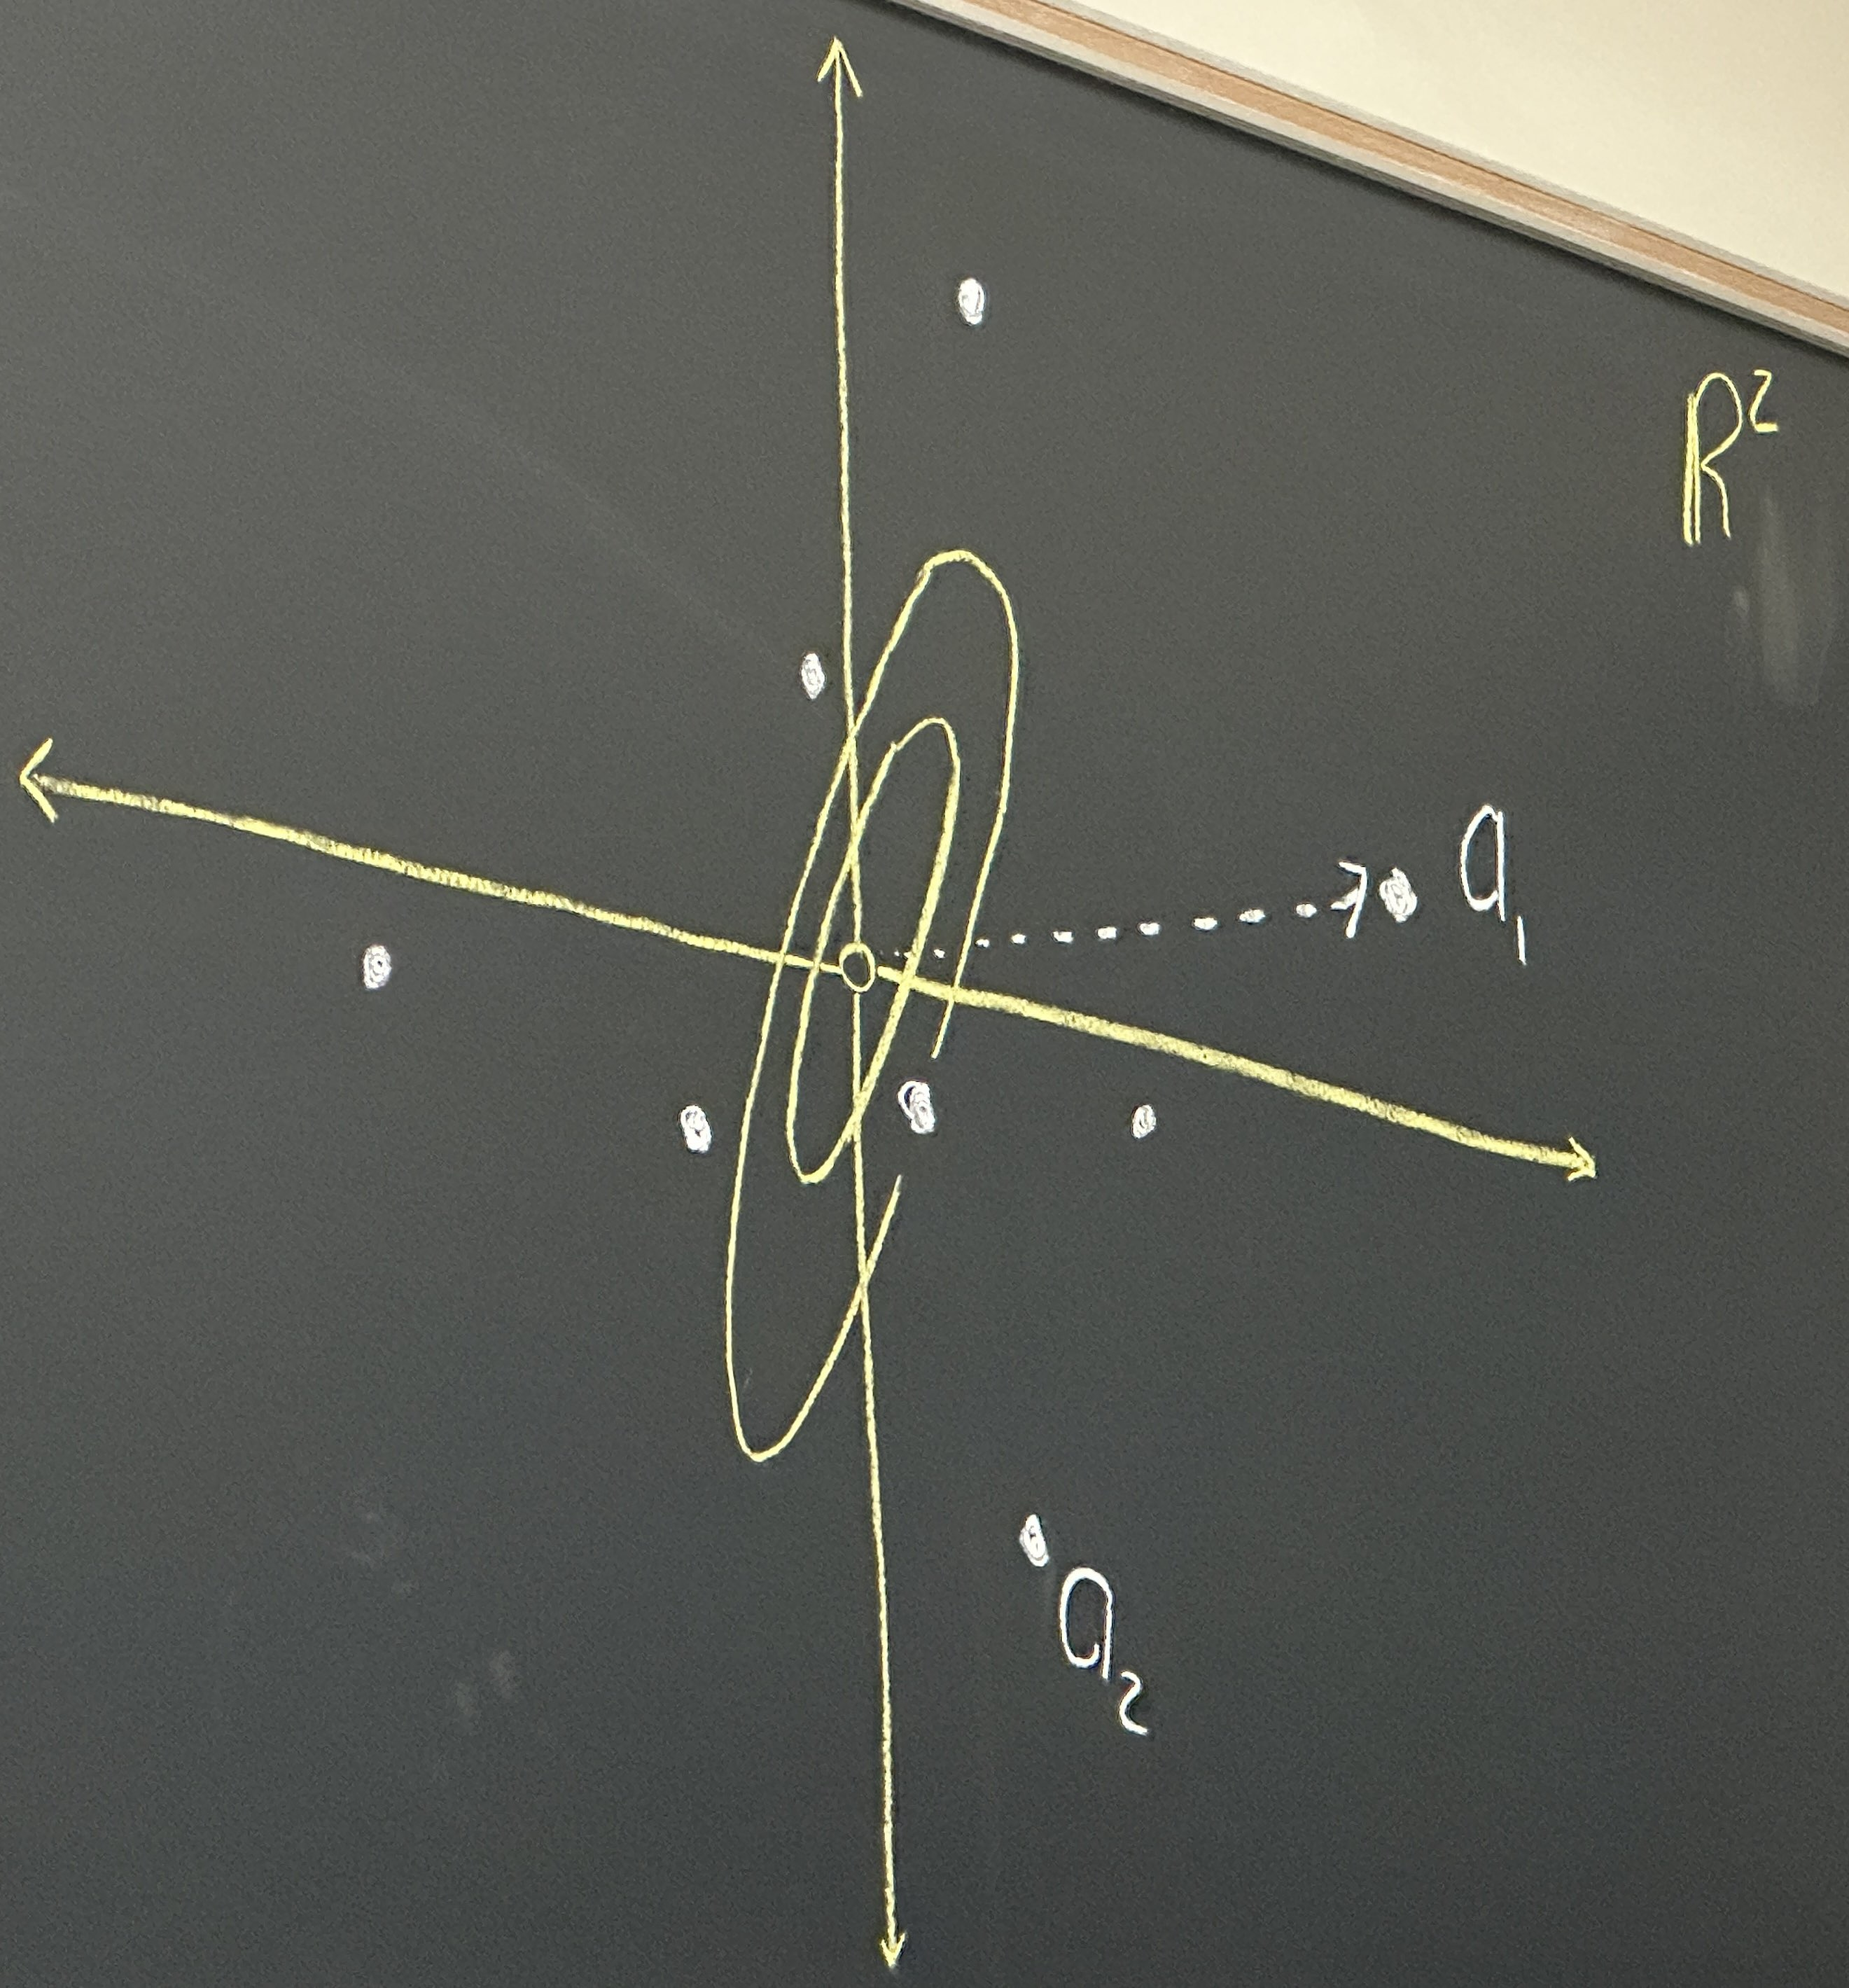
\includegraphics[scale=0.1]{lectures/wk10/img/ellipsoids.jpeg}
    \caption{Ellipsoids}
    \label{fig:ellipsoid}
\end{figure}

\subsubsection{Criteria to optimize j(n)}
\begin{enumerate}
    \item We want to choose $j$ at step $n$ to minimize $\E_{Y_n = y_n}(H[X\mid y_n, Y^{(n-1)}])=H[X\mid Y^{(n)}]$
    \item We want to choose $j(n)$ to maximize $I[X; Y^n \mid Y^{(n-1)}]$.
    \item We want to choose $j(n)$ to change your distribution the most, to maximize how much we expect the distribution to change (Information gain) after you ask the question $$\E_{Y_n = y_n}[D(\underbrace{p_{X\mid y^n, Y^{(n-1)}}}_{p_{n\mid y_n}} \| \underbrace{p_{X\mid Y^{(n-1)}}}_{p_{n-1}})]$$ where $p_{n\mid y_n}$ is the posterior and $p_{n-1}$ is the prior.
\end{enumerate}

We note that all 3 of the above criteria are equivalent. \textit{Proof:}
\begin{enumerate}
    \item Choose $j(n)\st$ it is the $\argmin_k\{\E_{Y_n(k) = y_n(k)}(H[X\mid y_n(k), Y^{(n-1)}])\}$ over all $k$th questions being asked.
    Note that this is the same as 
    $\argmin_k\{H[X\mid Y_n(k), Y^{(n-1)}]\}$
    \item $\argmin_k\{H[X\mid Y^{(n-1)}] - H[X\mid Y_n(k), Y^{(n-1)}]\}=\argmin_k\{I[X; Y_n(k)\mid Y^{(n-1)}]\}$
    Interpretation: You are greedily trying to maximize the amount of information gained.
    \item $$
    I[X; Y_n(k)\mid Y^{(n-1)}] 
    = D(p_{X, Y_n(k)\mid Y^{(n-1)}} \| \underbrace{p_{X\mid Y^{(n-1)}}}_{p_{n-1}} p_{Y_n(k)\cancel{\mid Y^{(n-1)}}})
    $$
    We started out by writing out mutual information as a KL divergence between the joint and the product of the marginals. But we note that the second marginal distribution in the product (2nd param of the KL Div.) is independent and thus can be removed. Thus we get:
    \begin{align*}
    &= \E_{X, Y_n(k)\mid Y^{(n-1)}}\left[\log\left(\frac{p_{X, Y_n(k)\mid Y^{(n-1)}}}{p_{X\mid Y^{(n-1)}} p_{Y_n(k)}}\right)\right]
    \\
    &= \E_{Y_n(k)\cancel{\mid Y^{(n-1)}}}\left[\E_{X\mid y_n, Y^{(n-1)}}\left[\log\left(\frac{p_{X, Y_n(k)\mid Y^{(n-1)}}}{p_{X\mid Y^{(n-1)}} p_{Y_n(k)}}\right)
    \right]
    \right]
    \\
    &= \E_{Y_n(k)}\left[\E_{X\mid y_n, Y^{(n-1)}}\left[\log\left(
    \frac{
        p_{Y_n(k)\mid Y^{(n-1)}}
        p_{X\mid Y_n(k), Y^{(n-1)}}
    }{p_{X\mid Y^{(n-1)}} p_{Y_n(k)}}\right)
    \right]
    \right]
    \\
    &= \E_{Y_n(k)}\left[\E_{X\mid y_n, Y^{(n-1)}}\left[\log\left(
    \frac{
        p_{Y_n(k)}
        p_{X\mid Y_n(k), Y^{(n-1)}}
    }{p_{X\mid Y^{(n-1)}} p_{Y_n(k)}}\right)
    \right]
    \right]
    \\
    &= \E_{Y_n(k)}\left[\E_{X\mid y_n, Y^{(n-1)}}\left[\log\left(
    \frac{
        p_{Y_n(k)}
        p_{X\mid Y_n(k), Y^{(n-1)}}
    }{p_{X\mid Y^{(n-1)}} p_{Y_n(k)}}\right)
    \right]
    \right]
    \\
    &= \E_{Y_n(k)}\left[\E_{X\mid y_n, Y^{(n-1)}}\left[\log\left(
    \frac{
        p_{Y_n(k)}
        p_{X\mid Y_n(k), Y^{(n-1)}}
    }{p_{X\mid Y^{(n-1)}} p_{Y_n(k)}}\right)
    \right]
    \right]
    \end{align*}
    Thus since $I[X; Y_n(k)\mid Y^{(n-1)}] = \E_{Y_n(k) = y_n(k)}[D(\underbrace{p_{n, y_n}}_{p_{X\mid y_n, Y^{(n-1)}}} \| \underbrace{p_{n-1}}_{\text{posterior given $Y^{(n-1)}$}})]$.
\end{enumerate}
Fun discussion problem: instead of an analytical solution as done below, utilize a decision tree to get an approximate solution.

Model:
$$
X\sim \cN(\mu, \Sigma_0)
$$
each question $j: q_j: a_j^\top X + \varepsilon = Y(j)$, with $\varepsilon\sim\cN(0, \sigma_j^2)$

for a fixed set of $m$ questions: $\{q_j\}_{j=1}^m$.

\begin{equation}
    q_j : Y(j) = a_j^\top X + \varepsilon
\end{equation}

This gives you a confidence interval which with high probability, you expect the true $X$ to lie when projected within the space -- you are constraining the projection of $X$ (with noise) onto a specific direction which changes the distribution. 

Since every variable in this problem is gaussian and linear, we understand how the posterior updates after each observation.

Also, a Gaussian can be uniquely identified with 2 pieces of information: $\mu, \sigma$. For a MVG, the entropy is solely dependent on the covariance matrix, so we simply need to observe how that updates.

Suppose: $p_{n-1}(X) = p(X\mid y^{(n-1)}) \sim \cN(\mu_{n-1}, \Sigma_{n-1})$.\\
Observe: $Y_{n}(j) = y_n(j) = a_j^\top X + \varepsilon$.\\
Posterior: 
\begin{align*}
p_{n}(X) 
&= p(X\mid y_n(j), y^{(n-1)}) 
\\
&\propto 
\underbrace{p_{Y_{n}{(j)}}(y_n\mid x, \cancel{Y^{(n-1)}})}_{\text{given $x$: } Y_n(j)\mid x\sim\cN(a_j^\top x, \sigma_j^2)}
p(X=x\mid y^{(n-1)})
\\
&\propto \underbrace{\exp(-\frac12 \left( 
\frac{(y-a_j^\top x)^2}{\sigma_j^2}
+
(x-\mu_{n-1})^\top \Sigma_{n-1}^{-1} (x-\mu_{n-1})
\right))}_{\ldots}
\end{align*}
where we took out the quadratic terms in $x$.

\subsubsection{Rank 1 updates to the Precision Matrix}
$$
x^\top 
\underbrace{(\frac1{\sigma_j^2}a_ja_j^\top + \Sigma_{n-1}^{-1})}_{\Sigma_0^{-1}}
x
$$

where $\Sigma_0^{-1}\implies \Sigma_n=(\Sigma_{n-1}^{-1} + \frac1{\sigma_j^2}a_ja_j^\top)^{-1}\indep Y^{(n)}$

and where $+ \frac1{\sigma_j^2}a_ja_j^\top$ is a rank 1 update to the precision, $P=\Sigma^{-1}$.

In statistics, the precision matrix or concentration matrix is the matrix inverse of the covariance matrix or dispersion matrix, $P=\Sigma^{-1}$. ${ }$ For univariate distributions, the precision matrix degenerates into a scalar precision, defined as the reciprocal of the variance, $p=\frac{1}{\sigma^2} \cdot$.

\subsubsection{Relating back to Entropy}
\vspace{-1em}
\begin{align*}
    H[X\mid Y^{(n)}] 
    &= \frac{d}2\ln(2\pi e)+\frac12\ln(\det(\Sigma_n))
    \\
    &\mapsto
    I[X; y_n(j)\mid Y^{(n-1)}]
    \\
    &= H[X\mid Y^{(n-1)}] - H[X\mid Y^{(n)}]
    \\
    &= \frac{d}2\ln(2\pi e)+\frac12\ln(\det(\Sigma_{n-1}))
    -\frac{d}2\ln(2\pi e)-\frac12\ln(\det(\Sigma_{n\mid j(n)}))
    \\
    &= \frac12\ln(\frac{\det(\Sigma_{n-1})}{\det(\Sigma_{n\mid j(n)})})
\end{align*}

Note that:
\begin{align*}
& \det\left(\Sigma_{n-1}^{1 / 2} \Sigma_{n \mid j(n)}^{-1} \Sigma_{n-1}^{1 / 2}\right) \\
& \det\left(\Sigma_{n-1}^{1 / 2}\left(\Sigma_{n-1}^{-1}+\frac{1}{\sigma_j^2} a_ja_j^\top\right) \Sigma_n^{1 / 2}\right) \\
& \det\left(I+\frac{1}{\sigma_j}\left({\Sigma}_n^{1 / 2} a_j\right)\left({\Sigma}_n^{\frac{1}{2}} a_j^{\top}\right)\right)
\end{align*}

\begin{figure}[H]
    \centering
    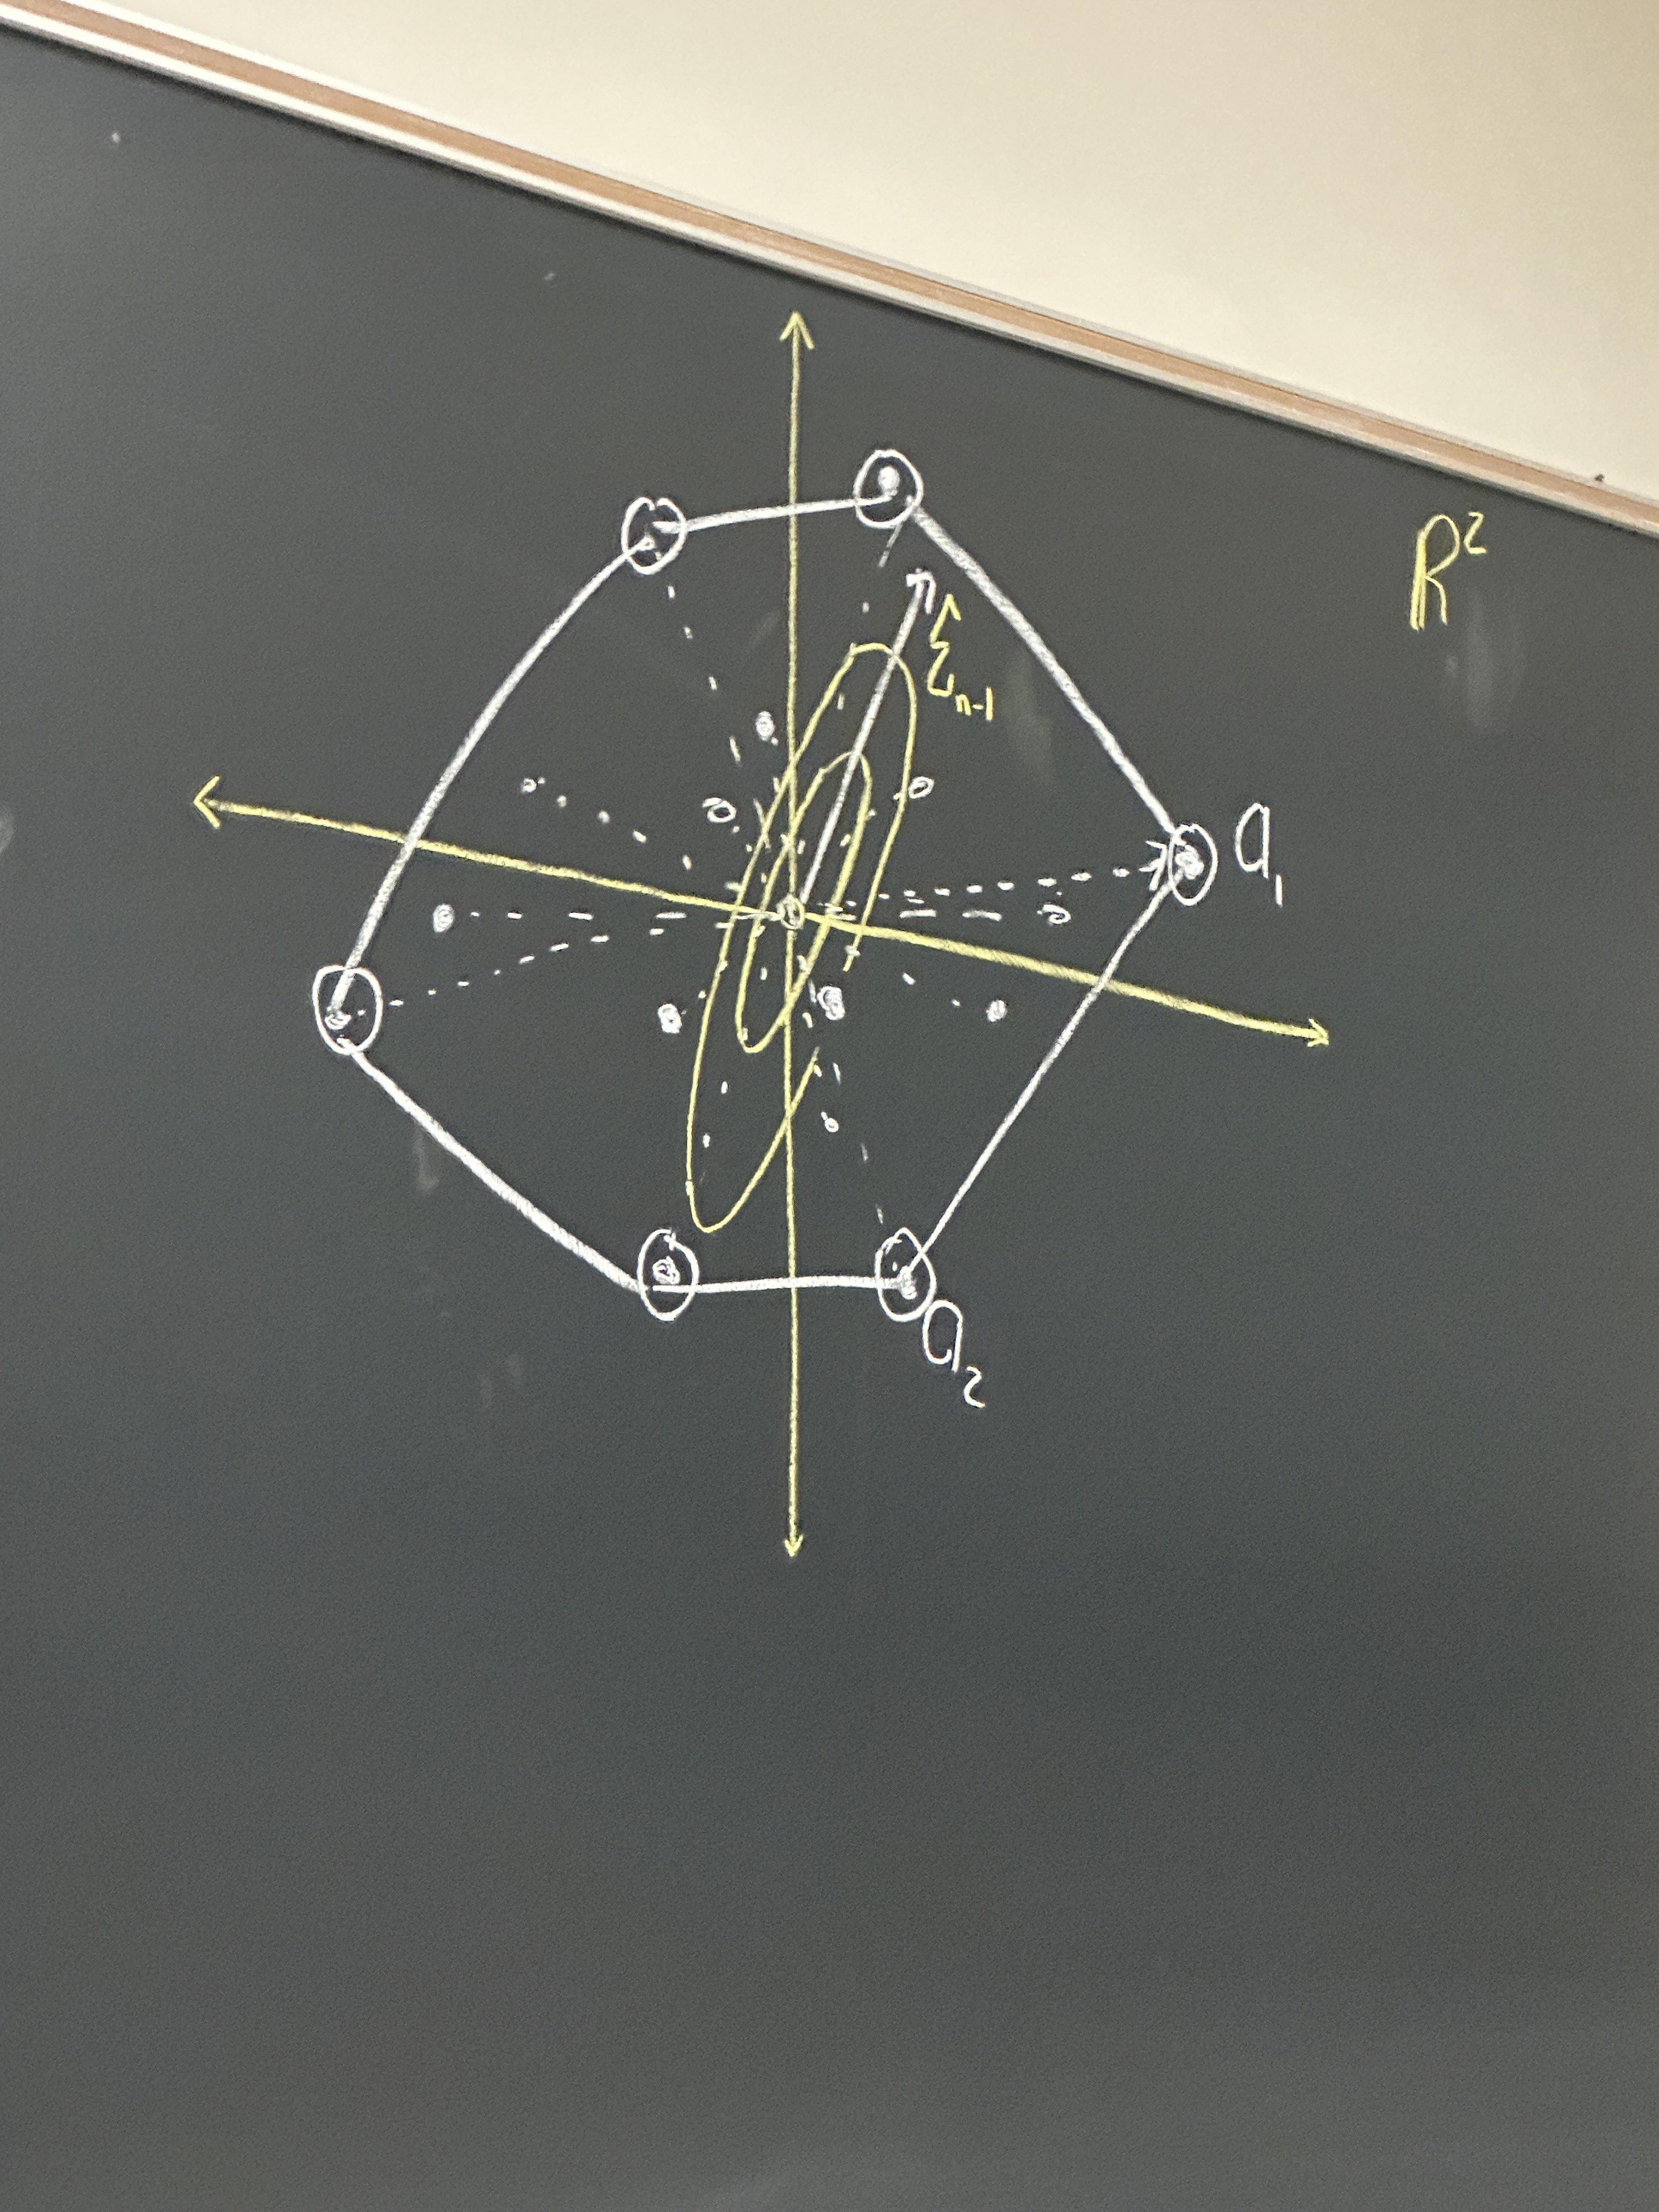
\includegraphics[scale=0.1]{lectures/wk10/img/constrainedEllipsoid.jpeg}
    \caption{Constrained Ellipsoid}
    \label{fig:constrained-ellipsoid}
\end{figure}

\subsection{Quadratic Programming is a Geometry Problem}
\begin{figure}[H]
    \centering
    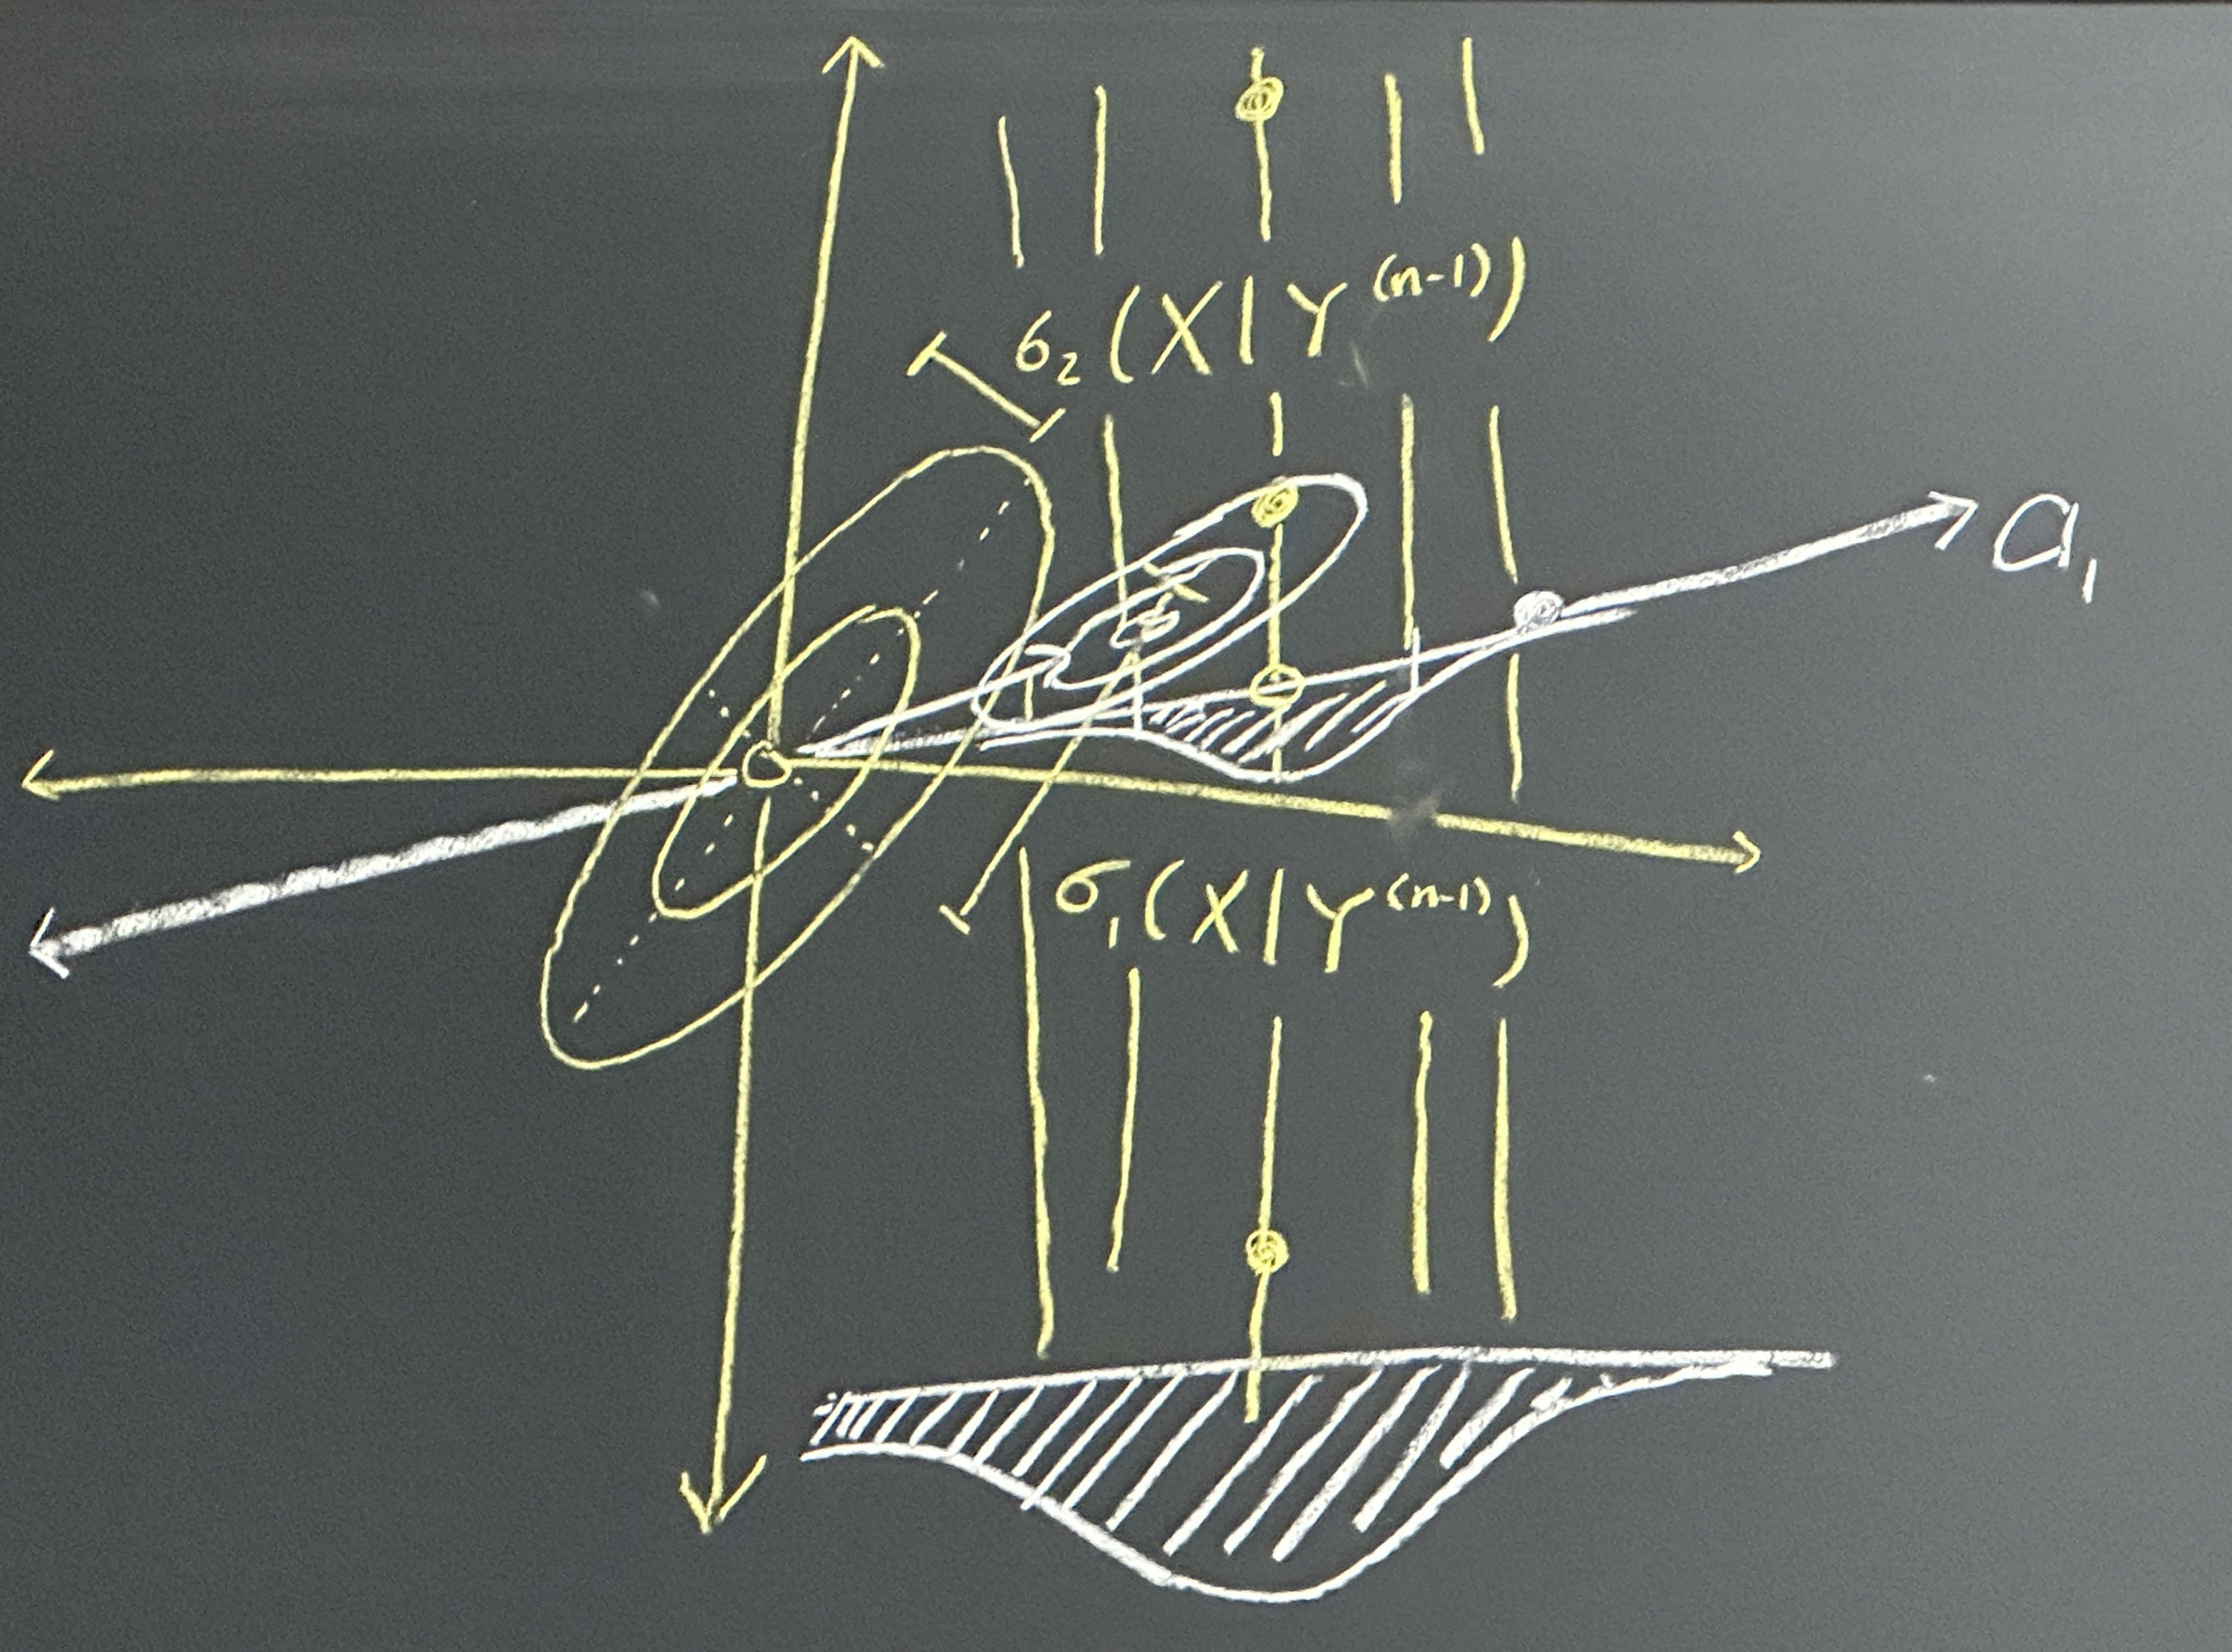
\includegraphics[scale=0.1]{lectures/wk10/img/QP.jpeg}
    \caption{Quadratic Program}
    \label{fig:quadratic-rogram}
\end{figure}
$$
\lambda_i(I+A)=1+\lambda_i(A)
$$

$$
\left(u u^{\top}\right)=
\begin{bmatrix}
    \\
    u
    \\ 
    \\
\end{bmatrix}
\begin{bmatrix}
  \quad  & u^\top & \quad
\end{bmatrix}
$$

\begin{itemize}
    \item Acquisition: pick $j(n)=\argmax_k \{\frac1\sigma_k^2 a_k^\top \Sigma_{n-1} a_k\}$
    \item Quadratic programming on a discrete set
\end{itemize}

\begin{equation}
\left(u u^{\top}\right) u=u\left(u^{\top} u\right)=\underbrace{\|u\|^2 u}_\lambda
\end{equation}

    \section{Thursday, March 21st: Stochastic Processes}
\subsection{Logistics}
\begin{enumerate}
    \item Peer Review -- due Today.
    \item Optional Reading posted -- T\&C 4, \underline{GP notes}.
    \item \underline{Enjoy Spring Break!}
\end{enumerate}

\subsection{Goals}
\begin{itemize}
    \item ($\cdot$) Processes
    \item ($\cdot$) \underline{Entropy Rates}
\end{itemize}

\subsection{Stochastic Process}
\begin{shaded}
A \textbf{stochastic process} $\{X_j\}_{j=1}^{\cdots}$ or $\{X(t)\}_{t}$ is indexed by ``time'', and is discrete or continuous.
\end{shaded}

\subsubsection{Joint distribution over a countable random vector}
There will be a joint distribution for any subset ($\{X_j\}_{j\in\mathcal{J}}$ or $\{X_j\}_{j\in\mathcal{J}}$) of variables, we have:
\begin{equation}
    \P(X_1=x_1,X_2=x_2, \ldots, X_n=x_n)
\end{equation}

There is no notion of 0 time -- it's arbitrary.

\subsubsection{Stationary of a Process}
\begin{shaded}
A process is \textbf{stationary} if $p(\{X_j\}_{j\in\mathcal{J}}=\{x_j\})=p(\{X_{j+s}\}_{j\in\cJ} = \{x_j\})$, if any set of samples is unchanged under time translation.
\end{shaded}

\subsubsection{Stationary Distribution}
\begin{shaded}
If a process, $\{X_j\}_{j=1}^{\cdots}$, is stationary then the corresponding Stationary Distribution is: 
\begin{equation}
p_{\text{stat}}(x) = P(X_j = x) \text{ for any $j$}
\end{equation}
\end{shaded}

\subsubsection{Ergodicity of Stochastic Processes}
\begin{shaded}
If a process, $\{X_j\}_{j=1}^{\cdots}$, is stationary then it is also \underline{Ergodic}: 
\begin{equation}
\label{ergodic-stat}
\E_{X\sim p_{\text{stat}}}[f(X)] = \Bar{f}_{\text{stat}}
\end{equation}

\begin{equation}
\label{ergodic-time}
\frac1n \sum_{j=1}^n f(X_j) = \Bar{f}_{\text{time}}(n) \stackrel{\small{n\to\infty}}{\to} \Bar{f}_{\text{time}}
\end{equation}
We expect the long-term avg to be concentrated and to converge.

The fact that \eqref{ergodic-stat} and \eqref{ergodic-time} are the same, $\Bar{f}_{\text{stat}}=\Bar{f}_{\text{time}}$, is what makes us ergodic.
\end{shaded}

\subsection{Markov Process}
A random process whose future probabilities are determined by its most recent values. A stochastic process $X(t)$ is called Markov \\
if $X(t+s),\quad s>0$ is conditionally $\indep$ of $X(t-h),\quad h>0$ given $X(t)$.
\begin{shaded}
The future is conditionally independent of the past given the present.
\end{shaded}

\begin{equation}
\operatorname{Pr}\left(X_{n+1}=x_{n+1} \mid \underbrace{X^{(n)}}_{
X_{n}, X_{n-1}, \ldots X_1}=x^{(n)}\right)
=
\underbrace{P\left(X_{n+1}=x_{n+1} \mid X_{n}=x_n\right)}_{\text{Transition prob.: } 
P_{i, j}^{\blue{(n)}}=P\left(X_{n+1}=i \mid X_n=j\right)}
\end{equation}

\subsubsection{Time Autonomous}
\begin{equation}
\Pr\left(X_{n+i}=i \mid X_{n}=j\right)=\Pr\left(X_2=i\mid X_1=j\right) 
\quad
\forall{i, j} \text { and } n. 
\end{equation}

\subsection{Transition Matrix}
The matrix $P$ has entries $P_{i, j}$ which give you the probability of going from $j$ at the present to $i$ in the future. That is, $P_{i,j}=\Pr(X_{n+1}=i\mid X_n=j), \quad P =\begin{bmatrix}
    \mid & \mid & & \mid \\
    p_1 & p_2 & \ldots & p_{|\cX|} \\
    \mid & \mid & & \mid
\end{bmatrix}$
with the $j$th column being the conditional distribution of the future given the present.

\begin{important}
Note that we use the following convention: this matrix is column-stochastic.
\end{important}

\begin{equation}
    \Pr(X^{(n)} = x^{(n)}) = 
    \underbrace{\left(
    \prod_{j=1}^n \P_{X_{j+1} X_j}
    \right)}_{\Pr(X^{(n)} = x^{(n)} \mid X_1=x_1)}
    p(X_1=x_1)
\end{equation}
where $p(X_1=x_1)$ is the initial distribution for the probability of where I start.

\subsection{Irreducibility}
A discrete-time, discrete-state MC is \underline{irreducibile} if
$\forall x_1=i, x_n=j \quad\exists$ a path $x^{(n)} = \{i, \ldots, j\}\st P(X^{(n)} - x^{(n)} \mid X_1 = i)>0$.

\subsection{Aperiodic}
A discrete-time, discrete-state MC is \underline{aperiodic} if
it's period is 1.

\subsubsection{Period}
A Period of the process is its GCD of the length of all cycles:
$$x^{(n)}  = \{x_1,x_2,\ldots, x_1\},\quad  P(X_n=x_n \mid X_1 = x_1)>0$$

\begin{figure}[H]
    \centering
    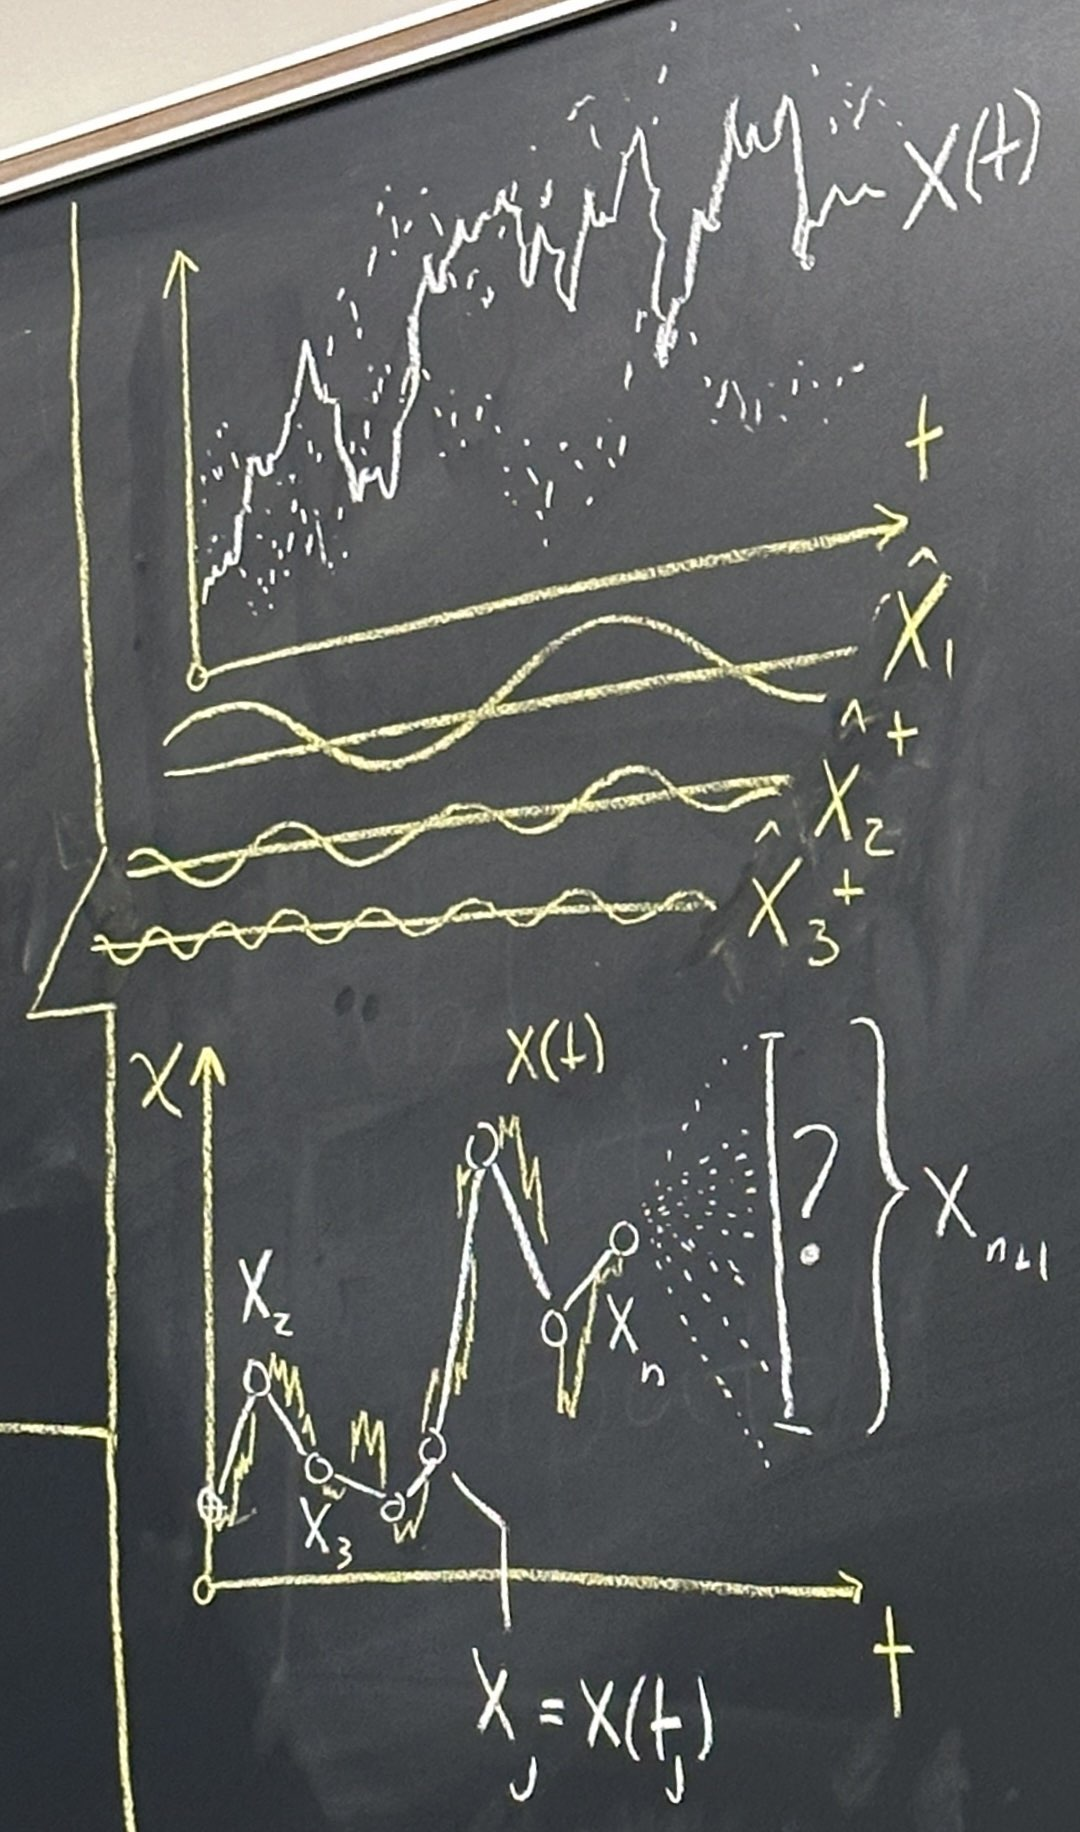
\includegraphics[height=25pc,width=40pc]{lectures/wk10/img/lec19_sp.jpeg}
    \caption{Various periods of Stochastic Processes}
    \label{fig:stoch-procs}
\end{figure}

\subsection{Perron-Frobenius Theorem}
If $P$ is column-wise Stochastic (transition for a $d-t, d-s$ MC) that is \underline{irreducible} \& \underline{aperiodic} then:

it converges to a \underline{unique stationary} distribution from any initial distribution, is stationary if initialized with $P_{\text{stat}}$, is \underline{ergodic}.


\begin{enumerate}
    \item $\exists$ a simple (A simple eigenvalue is an eigenvalue with multiplicity one -- the eigenvalue is unique) largest (in magnitude) eigenvalue $\lambda_{\max}(P)\in\R^+$.
    \item It's corresponding eigenvector $v_{\max}(P)\quad v_{\max}(x) \geq 0$ ($v \in \R^{+|\cX|})$
\end{enumerate}


Tldr;\\
A real square matrix with positive entries has a unique eigenvalue of largest magnitude and that eigenvalue is real ($\lambda\in\R$).

\subsection{Gershgorin Disk Theorem}
If $A\in \C^{n\times n}$ (or for simplicity, we will just provide a proof for $A\in \R^{n\times n}$), then $\lambda_j(A)\in \cup_{j=1}^n D(a_{jj}, \sum_{i\neq j} |a_i|)$

$
\sum_{i\neq j} |p_{ij}| = \sum_{i\neq j} p_{ij} = 1 - p_{jj}
$

This gives us that $|\lambda_j(P)|\leq1$.

$\therefore\quad \lambda_{\max}(P)=1$

$|\lambda_j(P)|=1\quad$ (if $j\geq2$).

\hrulefill

\begin{algorithm}
\caption{Algorithm for $p_0: p_n\stackrel{n\to\infty}\to \R$}
\begin{algorithmic}
\State \textbf{Initialize: } $\Pr(X_0=x)=p_0$.
\State \textbf{Find: } $p_n^{(x_n)}=\Pr(X_n=x_n)=\displaystyle\sum_{x_{n-1}}
\underbrace{\Pr(X_n=x_n\mid X_{n-1}=x_{n-1})}_{P_{x_n, x_{n-1}}} \underbrace{\Pr(X_{n-1}=x_{n-1})}_{P_{n-1}^{(x_{n-1})}}$
\Ensure Matrix columns add to 1.
\While{stopping criteria not met}
\State $p_n \gets Pp_{n-1}$
\State $p_n \gets P^n p_{0} = V\Lambda^{n} VV^\top p_0=V_{\max}(VV_{\max}^\top p_0)+\cO(\lambda_2^n)
= V_{\max}(\underbrace{\mathbbm{1}^\top p_0}_1)+\cO(\lambda_2^n)
= V_{\max}+\cO(\lambda_2^n)
$
\EndWhile
\State \Return $p_n$
\end{algorithmic}
\end{algorithm}

\subsection{Entropy Rate}
% pls help





Define $H'[\cX]=\displaystyle\lim_{n\to\infty} H[X_n \mid X^{(n-1)}]$.
\begin{enumerate}
    \item If the process is stationary then the sequence $H[X_n\mid X^{(n-1)}]$ is non-increasing and converges.
    \begin{shaded}
        \begin{proof}
        Undoing a conditioning should increase entropy:
            \begin{align*}
                H[X_n\mid X^{(n-1)}] 
                &=
                H[X_n \mid X_{n-1}, X_{n-2},\ldots,X_{2},X_{1}]
                \\
                &\leq H[X_n \mid X_{n-1}, X_{n-2},\ldots,X_{2}]
                \\
                &= H[X_{n-1} \mid X_{n-2}, X_{n-3},\ldots,X_{1}]
                &&[\text{Invariant under time shifts}]
                \\
                &= H[X_{n-1}\mid X^{(n-2)}]
                \\
                \underbrace{H[X_n\mid X^{(n-1)}]}_{>0}
                &\leq H[X_{n-1}\mid X^{(n-2)}]
                &&[\text{non-incr seq + bounded below $\implies$ conv.}]
            \end{align*}
        \end{proof}
    \end{shaded}
    \item The limit of the new entropy (the cndtl entropy in the future given the past) is $H[\cX]=H'[\cX]$.
    \begin{shaded}
        \begin{proof}
            \begin{align*}
                H[\cX] 
                &=
                \lim_{n\to\infty}\frac1n H[X^{(n)}] 
                = \lim_{n\to\infty} (\frac1n\sum_{j=1}^n H[X_j\mid X^{(j-1)}])
                \to H'[X]
            \end{align*}
        \end{proof}
    This can also be understood (the difference between the observed value of a variable at time $t$ and the optimal forecast of that value based on information available prior to time $t$) the innovation.
    \end{shaded}
\end{enumerate}

    \section{Tuesday, April 2nd}
\subsection{Logistics}
\begin{itemize}
    \item Review Reviews due Today
    \item Project Draft due next week, Thursday
    \item Reading (Ch. 4), post by Thurs
    \item Quiz 6 on Thurs: First half of chapter  4.1, 4.2 (Entropy rates and markov chains). Note that 4.4 and Mixing Inequalities (and thermodynamics) will be on the next quiz (not this upcoming one).
\end{itemize}

\subsection{Why cover Stochastic Processes}
If our end goal is to talk about communication and channels, why divert to processes?

\begin{shaded}
Answer: Stochastic Processes are a natural model for the process that generates the messages we want to send. Many messages like audio, video, text (sequence of characters with a distribution of next possible characters as opposed to future character popping out of nowhere), etc can be modeled as a process evolving over time.
\end{shaded}

This helps induce specific structural assumptions on joint dist. of possible messages, where assumptions $\Rightarrow$ results.

\subsection{Entropy Rates Review}
Stochastic Processes, $\cX$ ensemble (both the space of what you can send and their respective probabilities), $\{X(t)\}_t\sim$ joint distribution.


$$
H[\cX] = \lim_{n \rightarrow \infty} \frac{1}{n} H[X^{(n)}]
$$ where $X^{(n)} = \{X_1, X_2, \ldots, X_n \}, X_j = X(t_j)$

if there is, each time I take a step Iadd additional randomness. Thus:
\begin{shaded}
Entropy increases as $n\to\infty$.
\end{shaded}

This is the sample-wise uncertainty/randomness in the trajectory (for long trajectories). This has a dual perspective if you approach the problem geometrically. As we have longer processes, the stochastic process should grow as a fn of $n$ as $n$ increases.

\begin{figure}[H]
    \centering
    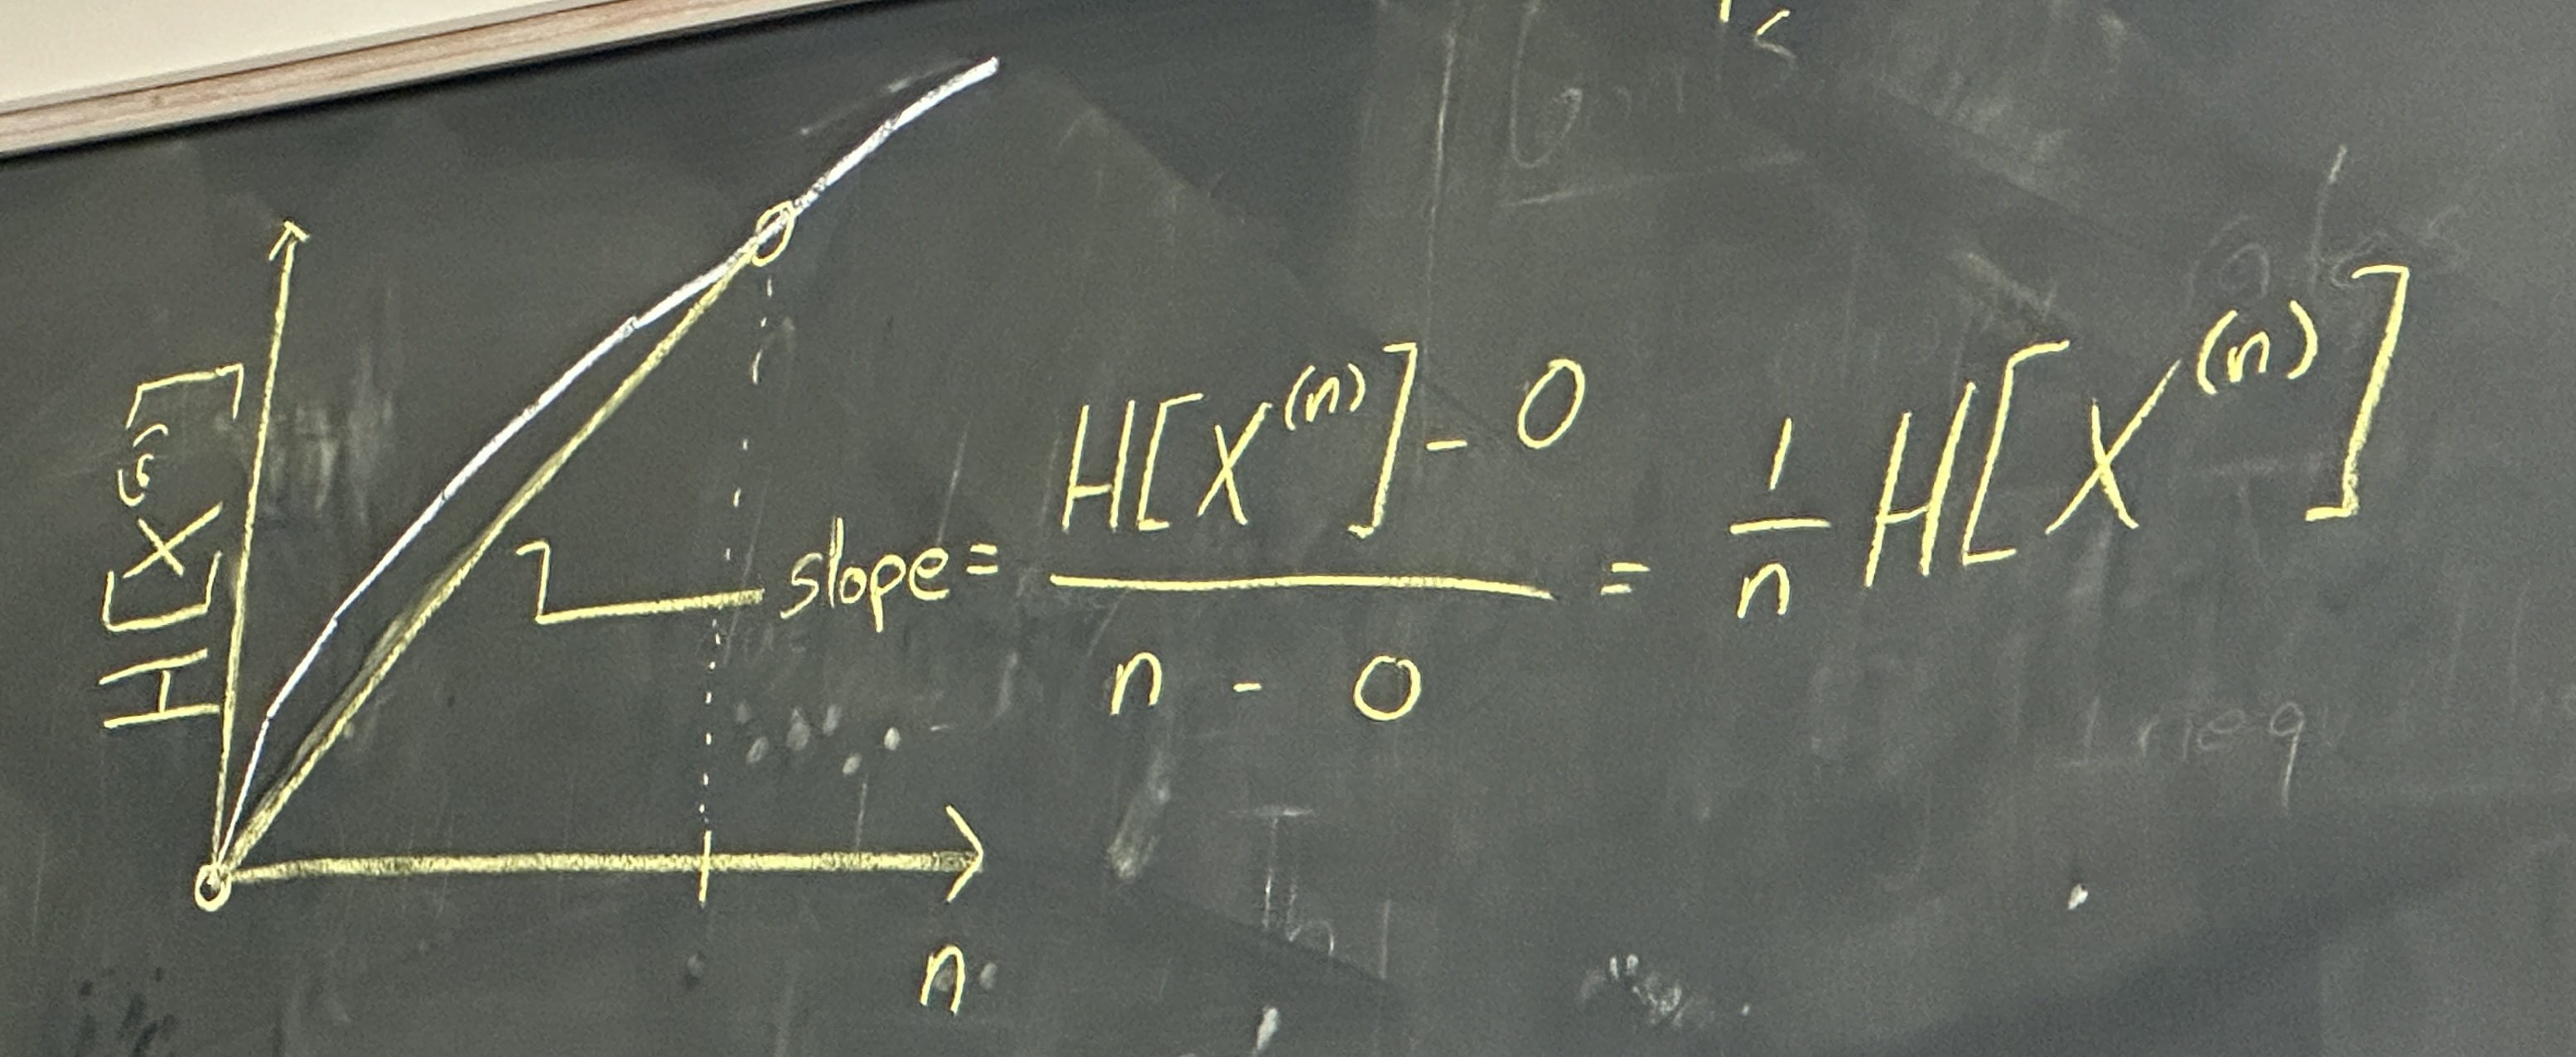
\includegraphics[scale=0.15]{lectures/wk11/img/entropy_increasing.jpg}
    \caption{We examine the secant line}
    \label{fig:enter-label}
\end{figure}

We use the word rate since this is the long term rate of growth in the joint entropy of a long trajectory, $H[X^{(n)}]$.

\begin{itemize}
\item $H[X_{n+1} \mid X^{(n)}]$
\item 
    \begin{align*}
    H[X^{(n+1})] - H[X^{(n)}] 
        &= (H[X^{(n)}]+H[X_{n+1}\mid X^{(n)}]) - H[X^{(n)}]
    \\
        &= H[X_{n+1}\mid X^{(n)}]
    \end{align*}
\end{itemize}

\subsubsection{Alternate defn. of Entropy Rate}
\begin{align*}
    H'[\cX]
    &= \lim_{n\to\infty} H[X_{n+1} \mid X^{(n)}]
\end{align*}

If $\cX$ is stationary $\implies H[\cX]=H'[\cX]$. A stationary process means if I sample at a sequence of time, the joint distributions would not change under time (time-invariance).

\subsection{Application of Entropy Rate}
Recall how we studied compression earlier in the semester.

We have messages $\{X(t_j)\}_{j=1}^n, X^{(n)}\sim \cX$.

We have Code: $C(X^{(n)})\to$ string of $d$-ary characters.
\begin{itemize}
    \item ($C_j\in \{\text{instantaneous codes $\cX$}\}$)
\end{itemize}
Note that `dits' is the equivalent of `bits' for $d$-ary character as opposed to binary.

$L(C)=\E_{X^{(n)}}[|c(x^{(n)})|], \quad L^*(\cX)=\min_{c\in C}\{L(x)\}\in [H_d[X^{(n)}], H_d[X^(n)] + 1]$.

$L^*$ should be growing as we try to encode longer messages, as we increase $n$.

This leads to $L_n^*(\cX) = \frac1n L(\cX)$.

$$\lim_{n\to\infty} \frac1n L^*(\cX)\in\lim_{n\to\infty} \frac1n(H_d[X^{(n)}] + [0, 1]) \to H_d[\cX] + \cO\left(\frac1n\right)$$

\subsection{Innovation Rates}
\begin{align*}
\text{Entropy Rate of process } 
&= H[\cX] 
\\
&= \text{ a minimum (best rate), the number of dits per sample needed 
}
\\
&
\quad\quad
\text{
on average to specify a trajectory.}\\
&= \text{ new info needed to specify $X_{n+1}\mid X^{(n)}$} (on average)
\end{align*}

Everything above is in-scope for Quiz 6.

\hrulefill

Everything below is in-scope for Quiz 7:
\subsection{Mixing Inequalities (Markov Chains)}
\begin{itemize}
    \item $\cX$ is a (Discrete-Time) M.C., $X(0)\sim p_0, Y(0)\sim q_0, X_n\sim p_n, Y_n\sim q_n$
\end{itemize}
\begin{enumerate}
    \item $D(p_{n+1} \| q_{n+1}) \leq D(p_n \| q_n)$, so $\{D(p_n\|q_n)\}$ is monotonically nonincreasing. `If they follow the same rules, they should forget how they were initialized.'
    
    Moral: 
    \begin{shaded}
    The process \textit{mixes}: the cdtl. distribution of the current state gets more similar to the cdtl. distro. initialized differently.
    \end{shaded}
\end{enumerate}
\begin{proof}
Like most proofs in this class, if it does not involve Jensen's/convexity, we use Chain Rule:
\begin{align*}
D(p_{X_{n+1}, X_n} \| q_{Y_{n+1}, Y_n}) 
&= \begin{cases}
    \text{Past:}
    & 
    D(\underbrace{p_{X_n}}_{p_n} \| \underbrace{q_{Y_n}}_{q_n}) + \underbrace{D(p_{X_{n+1} \mid X_n} \| q_{Y_{n+1}\mid Y_n})}_{0 \text{ since they follow the same transition probabilities}}
    \\
    \text{Future:}
    & 
    D(%\underbrace
    {p_{{n+1}}}
    %_{p_n}
    \| %\underbrace
    {q_{{n+1}}}
    %_{q_n}
    ) + \underbrace{D(p_{X_{n} \mid X_{n+1}} \| q_{Y_{n}\mid Y_{n+1}})}_{\geq0}
\end{cases}
\\
&= \begin{cases}
    \text{Past:}
    & 
    D(p_n\|q_n)
    \\
    \text{Future:}
    & 
    D(%\underbrace
    {p_{{n}}}
    %_{p_n}
    \| %\underbrace
    {q_{{n}}}
    %_{q_n}
    ) 
    - \underbrace{\ldots}_{\geq0}
    + \underbrace{D(p_{X_{n} \mid X_{n+1}} \| q_{Y_{n}\mid Y_{n+1}})}_{\geq0}
\end{cases}
\\
D(%\underbrace
    {p_{{n+1}}}
    %_{p_n}
    \| %\underbrace
    {q_{{n+1}}}
    %_{q_n}
    )
    &\leq 
    D(%\underbrace
    {p_{{n}}}
    %_{p_n}
    \| %\underbrace
    {q_{{n}}}
    %_{q_n}
    ) 
\end{align*}
\end{proof}

\subsection{What does it mean if your MC is Stationary}
It means you are irreducible and aperiodic and finite. Then $\exists p_s$ which is a stationary distributions. If you initialize $Y$ from the stationary then you stay there. Thus $D(p_{n+1}\| p_{s})\leq D(p_{n}\| p_{s})$, and $p_n\stackrel{n\to\infty}\to p_s\quad\forall p_s$.

\begin{equation}
    D(p_n\| p_{s}) \stackrel{n\to\infty}\to 0, \quad
    D(p_n\| q_{n}) \stackrel{n\to\infty}\to 0
\end{equation}

\subsection{Linkages to Data Processing}
\begin{enumerate}
    \item[2.] $I[X_{1} \| X_{n+1}) = I[X_{n+1} \| X_{1}] \leq I[X_1; X_n]=I[X_n; X_1]$, so: $\{I[X_1\|X_n]\}$ is monotonically non-increasing.

The longer you let this process run, the less information you have about the past.

The longer you let a MC run, the less information you have about where it started: ``the process forgets where it started''.
    \begin{itemize}
        \item Then: $H[X_1\mid X_{n+1}] \geq H[X_1\mid X_{n}]$.
        \item And if stationary: $H[X_{n+1} \mid X_1] \geq H[X_n \mid X_1]$. You will ultimately forget \textbf{everything} about where you started. It carries \textit{no} information about the far past.
    \end{itemize}
\end{enumerate}

\subsection{The second law of Thermodynamics}
\begin{itemize}
    \item $H[X_1\mid X_{n+1}] \geq H[X_1\mid X_n]?$

    Recall $I[A; B] = H[A] - H[A\mid B] = H[B] - H[B\mid A]$.
    
    DPI (Data Processing Inequality): $I[X_1; X_{n+1} \leq I[X_1; X_n].$
    
    $H[X_1] - H[X_1 \mid X_{n+1}]\leq
    H[X_1]  - H[X_1 \mid X_{n}]
    \implies
    $ 
    $ - H[X_1 \mid X_{n+1}]\leq
      - H[X_1 \mid X_{n}]
    $ 
    $  
    \implies
    H[X_1 \mid X_{n+1}]\geq
       H[X_1 \mid X_{n}]
       .
       \hfill\square
    $ 

    \item $H[X_{n+1}\mid X_1] \geq H[X_n\mid X_1]?$

    DPI: $I[X_{n+1}; X_{1} \leq I[X_n; X_1]$.
    
    $H[X_{n+1}] - H[X_{n+1} \mid X_{1}]
    \leq
    H[X_{n}] - H[X_{n} \mid X_{1}]
       .
    $ 

    If stationary by DPI: 
    \begin{align*}
        H[X_{n+1}] - H[X_{n+1} \mid X_1] &\leq H[X_n] - H[X_n \mid X_1] \\
        H[p_{x_{n+1}}] - H[X_{n+1}] &\leq H[p_{x_{n+1}}] - H[X_n \mid X_1] \\
        H(p_s) - H[X_{n+1} \mid X_1] &\leq H(p_s) - H[X_n \mid X_1] \\ 
        H[X_{n+1} \mid X_1] &\geq H[X_n \mid X_1]
    \end{align*}

    $H[X_{n+1}\mid X_1]
    \geq
    H[X_{n}\mid X_1]
    \hfill\square$
    
\end{itemize}




    \section{Thursday, April 4th}
\subsection{Logistics}
\begin{itemize}
    \item Review Reviews
    \item Discussion Posted
    \item Project Update due next Thursday
    \item Quiz 6 Today
\end{itemize}

\subsection{Information and Thermodynamics}
Consider the second law of thermodynamics, which states "entropy always increases". We want to formalize this. What exactly are we computing the entropy of? We need to take into account the random variable, distribution and the overall state of the system. Does it increase always or under certain assumptions?

The big question is if thermodynamic entropy can be related to the notion of entropy that we have developed so far. 

\subsection{Naive Approach}
Let's try a Markov Chain approach! We'll start simple with just two states and work in discrete time. Imagine a Markov chain with two states $\boxed1$ and $\boxed2$. Let's assume transitions $p_{11}, p_{12}, p_{21}$ and $p_{22}$ are all nonnegative. Assume WLOG that $p_{21}>>p_{11}>0$ and $p_{22} >> p_{12}>0$. 

Note that the steady state behaviour of this system basically sets $p^*_{22}=1$ and $p^*_{11} = 0$ in the limit of these two assumptions. We would like to say that the entropy of some quantity is increasing in time. 

Consider the entropy of $X(t)$. Clearly $H[X(t)] = 0$ in the limit since all of the probability mass is concentrated at $\boxed2$. However, imagine if we started the process with an initial uniform distribution? 

Then we have just decreased the entropy! We have designed a process that starts with maximal entropy and reduces all the way to $0$ entropy. 

\subsection{Thermodynamics}

What is Thermo? We are not talking about your average thermoflask here. It is a statistical theory for dynamics of macroscopic observable. It studies quantities of heat, energy, temperature and pressure. Microstate refers to the detailed model. However, this is completely intractable. You want to think about this as your average Tall drink in Starbucks. 

Mesoscopic states refers to "mid-sized" process. Think of this as your average Grande drink from Starbucks. 

Macroscopic state refers to the state where you average out the randomness and go to the limit of having infinite particles. Think of this as your average Venti drink from Starbucks. 

\subsection{Picking a System for the Mesoscopic State}
\subsubsection{Microscopic vs Mesoscopic vs Macroscopic}
\begin{figure}[H]
    \centering
    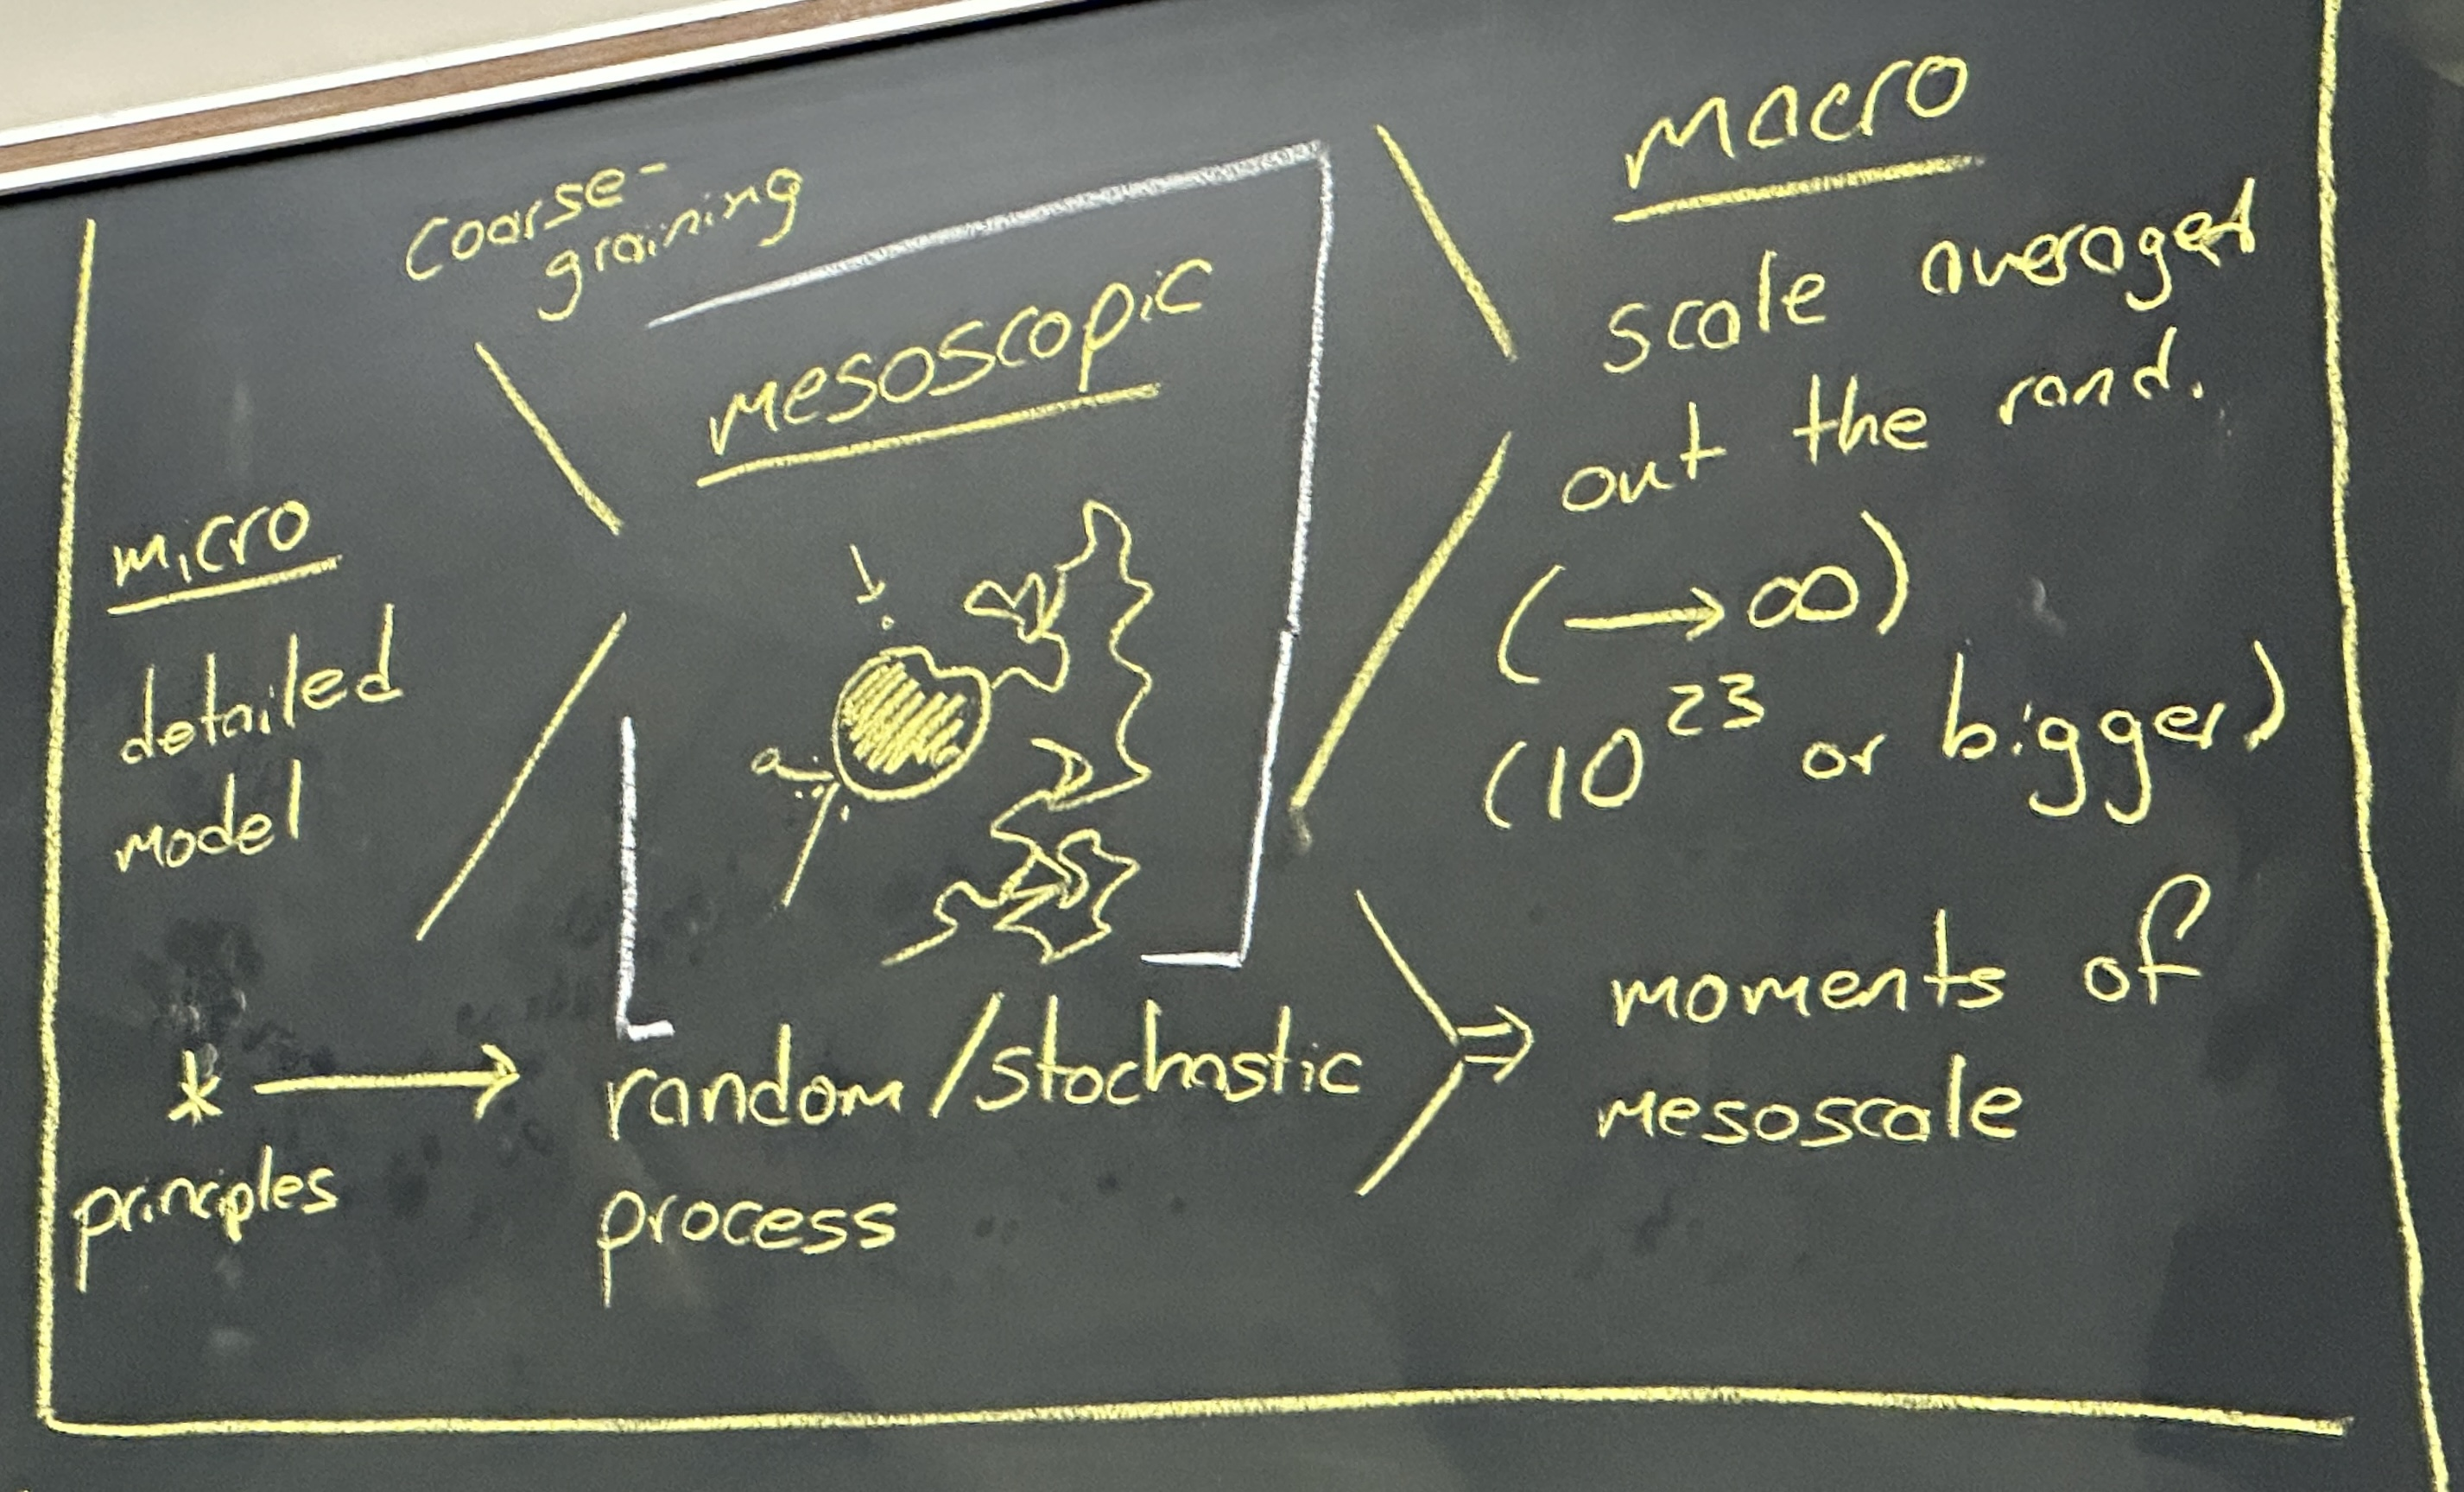
\includegraphics[scale=0.152]{lectures/wk11/img/meso.jpeg}
    % \caption{Caption}
    \label{fig:micro-meso-macro}
\end{figure}



\subsection{Continuous Time Markov Chains}
$X(t)$ is a jump process. 

\begin{itemize}
    \item Waiting times are exponentially distributed : $T_j \sim \Exp(\sum_{k\neq j} r_{kj})=\Exp(R_j)$.
    $R_j = \sum_{k \neq j} r_{kj}$

    \item Prob jump from $j \rightarrow k$ is $ \frac{r_{kj}}{R_j}$

    \item Then: transition rate matrix: $R = 
    \begin{cases}
        r_{ij} &= \mathrm{rate } j \rightarrow i \\
        r_{ii} &= -R_i = - \sum_{k \neq i} r_{k_i}
    \end{cases}
    $

    \item Master Equation: Let $p(t) = \mathrm{dist } X(t), X(0) \sim p(0)$ then: $ \dv{}{t}p(t) = Rp(t)$ so: $p(t) = e^{Rt} p(0)$

    \item Steady-State: $P_s$ s.t. if $X(0) \sim p_s, X(t) \sim p_s$ solution to $: Rp_s = 0$

    \item Flux-Balance: flux $j \rightarrow i = r_{ij} p(x_j, t)$

    \item Complex-Balance: $ \sum_{j \neq i} r_{ij} P_s(j) = R_i P_s(i) $

    \item Discretization: $p_n = \mathrm{dist } X_n = X(t_n)$
    if $t_n = n \Delta t$ then $X_n$ is a discrete time MC with transition prob matrix $P(\Delta t) = e^{R \Delta t}$
\end{itemize}

\begin{shaded}
What are the barebones addtl. assumptions to introduce to our stoch proc at the microscopic scale to satisfy sensible mesoscopic scale dynamics?
\end{shaded}

\subsection{Conservation Laws}
\begin{itemize}
    \item total mass is conserved
    \item momento (momentum) is conserved
    \item energy is conserved -- it cannot be created nor destroyed -- but \textit{why}? 
\end{itemize}

\subsection{Required Symmetries}
\begin{enumerate}
    \item If I knew every detail of the current state, then I would know the rule for how it changes $\implies$ dynamics only depend on the current-state.
    \item The process evolves in cts.-time.
    \item If we knew or could track all relevant d.o.f. then the dynamics would be \textit{time autonomous}.
    \item Time-Reversibility: Your dynamical rules (updates to your system) should be symmetric if you reverse time. This is what implies the conservation of energy.
\end{enumerate}

\subsection{Noether's Theorem}
Every continuous symmetry of the action of a physical system with conservative forces has a corresponding conservation law.

Translational symmetry $\mapsto$ Conservation of momentum.

Rotational symmetry $\mapsto$ Conservation of angular momentum.

Time-Translational symmetry $\mapsto$ Conservation of total energy.

% If your mesoscopic process is markov then your microscopic process will be Markov.
% 
If your microscopic process is markov then your mesoscopic process will be Markov.

    \section{Thursday, April 9th}
\subsection{Logistics}
\begin{itemize}
    \item Reading Posted (7.1 - 7.3)
    \item Discussion due Thurs
    \item Project Part 5 due Thurs.
    \item Quiz 6 retake tmrw.
    \item Quiz 7 Thurs: Only on \textbf{Mixing Inequalities}.
\end{itemize}

\subsection{Hierarchy of Models}
\subsubsection{Stochastic Thermodynamics}
Thermodynamics is a statistical theory which works across scales of physical systems. Today we will focus on the intermediate scale of Mesoscopic. This field is known as Statistical Thermodynamics or Stochastic Thermodynamics.

Recall the conserved principles we decided to enforce from last lecture:
\begin{enumerate}
    \item $\approx$Markov (assume time-scale separation/adiabatic limit allows us to assume memorylessness at this scale)
    \item Time is cts.
    \item Process is autonomous
    \item Some(?) form of time-reversal symmetry$^\ast$
    \begin{itemize}
        \item By enforcing the correct properties, we can conserve the correct properties. Today we will get more specific to this end.
        \item We could enforce a very strong form of symmetry and get results but these would not be \textit{interesting} results as we are then restricted to a very small subset which is the class of symmetric models.
    \end{itemize}
\end{enumerate}

\subsection{CT Review from Last Lecture}
Transition matrices can be constructed from the rate matrices through the matrix exponential: $p(t+\Delta t)=e^{R\Delta t}p(0)\implies p(t)=e^{Rt}p(0)$.

\subsection{Model}
We have CT finite (Discrete-State) MC which is autonomous (we know or can track all relevant d.o.f. for the dynamics).

We also want reversibility, microscopic reversibility: means any time $i\to j$, you can also go $j\to i$.\\
Thus if $r_{ij}>0\implies r_{ji}>0$.

\subsubsection{Stronger Symmetry}
\begin{important}
\begin{equation}
    r_{ij} = r_{ji}
\end{equation}
but this is \textit{too} limiting: it only yields $p_s\sim\Uniform$.
\end{important}

\subsubsection{A better Symmetry}
Examining the stationary distribution, we want symmetry in probability flux -- of steady-state ($r_{i j} p_{{s}_{j}} = r_{j i} p_{s_i} \forall{i, j}$): if $p=p_s$ where $p_s=\pi$ is the stationary distribution.

\subsubsection{Ensembled Indistinguishability is the same as Probability flux symmetry}
The former states: If $p(0)=p_s$ then it's not possible to distinguish a trajectory, run fwd in time from one run backwards in time.

Both are equivalent ways of saying that the stoch proc $X(t)$ obeys DBEs.

\subsection{Probability Fluxes}
\begin{align}
J_{ij}(p) & =r_{i j} P_j \\
\Big(\frac{d}{d t} P_i(t) & =\text { flux in - flux out }\Big)
\end{align}

\subsection{Stationarity:}
\subsubsection{Complex Balance:}
\begin{equation}
\underbrace{\sum_{j \neq i} r_{i j} P_{s_j}}_{\text{total in}} 
= \underbrace{\left[\sum_{j \neq_i} r_{j i}\right] 
P_{s_i}}_{\text{total out}}
\end{equation}

\subsubsection{Detailed Balance:}
\begin{equation}
r_{i j} p_{{s}_{j}} = r_{j i} p_{s_i} \forall{i, j}
\end{equation}

\subsection{Theorem}
A CT discrete-state (finite) MC satisfies DBEs if:
\begin{flalign}
    \text{at steady-state: } & J_{ij}(p_s) = J_{ji}(p_s)
    \label{eq:flux-at-steady-state}
    \\
    \text{time-reversal symmetry of the ensemble } 
    &
    \text{if initialized at steady-state.}
    \label{eq:time-reversal-symmetry-ensemble}
    \\
    \text{Defn.: $\E$[Production rate of a quantity $q$]} &= \sum_{i<j} \Delta q_{ij} \left(J_{ij}(p) - J_{ji}(p)\right)
    \label{eq:prod-rate}
    \\
    \text{Given $|C|$ cycles, you obeys DBEs} & \iff \sum_{j=1}^{|C|}\ln(\frac{r_{x_{j+1} x_j}
    }{r_{x_{j}, x_{j+1}}})=0
    \label{eq:cycle-sum-log-ratio-of-rates}
\end{flalign}
Note that all of these are 4 equivalent.

\subsection{Open System}
Imagine there are particles in a system (the particles can leave the system) and we want to track the current amount of particles in the finite and bounded reservoir at any given time. It is natural to utilize expectation for this task.

\begin{important}
What if eq. $\eqref{eq:prod-rate}$ is violated?
\end{important}

Then $\exists q\st$ the prod. at steady-state is $>0$.

Thus at steady-state, we expect the  quantity to grow but by defn. of the stationary state we know this must be true at all future times as well. If we are constantly pulling a positive amount from a bounded finite system, then we will eventually run out.

Since the stoch proc is ergodic, w.h.p., the total amnt. of quantity exchanged with the reservoir would grow w/o bound. Thus it is impossible for the reservoir to be bounded: the system is closed.

Thus at steady-state,  eq. $\eqref{eq:prod-rate}=0$ in any $q$.

\begin{align*}
\forall \Delta q_{ij} &= -\Delta q_{ji} 
\\
\sum_{j < i} \Delta q_{ij} \underbrace{\left(J_{ij}(p) - J_{ji}(p)\right)}_{=0} &= 0
\end{align*}
This shows that eq. $\eqref{eq:flux-at-steady-state}\implies\text{eq. }\eqref{eq:prod-rate}$.

\subsection{Forward Trajectory}
We use the notation:
\begin{align*}
    \{
    X^+(t)
    \}_{t=0}^T
    &= \{x_1, x_2, x_3, \ldots, x_n\}
\end{align*}
where $x_1=x(0), \quad x_n=x(T)$ with $\{\tau_1, \tau_2, \ldots, \tau_n\}$.

\subsection{Backwards Trajectory}
We use the notation:
\begin{align*}
    X^-(s)
    &= X^+(T-s)
\end{align*}
which implies that:
\begin{align}
    p_s(x_1)\prod_{j=1}^{n-1} \Bar{r}_{x_j} e^{-\Bar{r}_{x_j}\tau_j} \frac{r_{x_{j+1}, x_j}}{\Bar{r}_{x_j}}
    &= 
    p_s(x_n)\prod_{i=1}^{n} 
    e^{-\Bar{r}_{x_i}\tau_i} 
    % \frac{r_{x_{i+1}, x_i}}{\Bar{r}_{x_iJ}}
    \Bar{r}_{x_j} \\
    \implies \left(\prod_{j=1}^n \frac{r_{x_{j+1} x_j}}{r_{x_j x_{j+1}}} \right) \frac{p_s(x_1)}{p_s(x_n)} &= 1
\end{align}
If we choose $x_n=x_1$ then $\frac{p_s(x_1)}{p_s(x_n)}=1$ no matter what the stationary probabilites specifically are. We have a cycle since we have a path which ends where it starts $\implies$ so if we take a $\log$ on both sides then we get that eq. $\eqref{eq:time-reversal-symmetry-ensemble}\implies\text{eq. }\eqref{eq:cycle-sum-log-ratio-of-rates}$.

Finally we show that eq. $\eqref{eq:time-reversal-symmetry-ensemble}\implies \text{eq. }\eqref{eq:flux-at-steady-state}$:

The simplest trajectory is one which only takes a single step. Thus we get that:
\begin{align*}
    \frac{r_{x_2 x_1} p_s(x_1)}{r_{x_1 x_2} p_s(x_2)} &= 1
    \\
    \implies 
    r_{ij}p_{s_j}
    &= 
    r_{ji}p_{s_i}
\end{align*}
$\hfill\square$

This gives us much more than a nullspace el. of the rate matrix, $Rp_s=0$, as is given by the CBE.

\subsection{A cyclic property}
For any cycle, that is, a sequence of states $\{x_1, x_2, \ldots, x_n, x_{n+1}=x_1\}$, we must have:
\begin{equation}
    \sum_{j=1}^n \ln\left(\frac{r_{x_{j+1} x_j}}{r_{x_1 x_{j+1}}}\right)
    = 0
\end{equation}

\subsection{Line Integrals to define Energy as a quantity}
If you have a path $P_1=\{i, x_2, \ldots, x_{m-1}, j\}$ and a path $P_2=\{i, y_2, \ldots, y_{\ell-1}, j\}$.

\begin{align}
    \sum_{\stackrel{n=1}{P_1}}^m \ln\left(\frac{r_{x_{n+1} x_n}}{r_{x_n x_{n+1}}}\right)
    &= \sum_{\stackrel{n=1}{P_2}}^{\ell} \ln\left(\frac{r_{y_{n+1} y_{n}}}{r_{y_{n} y_{n+1}}}\right)
\end{align}

Then for the quantity $u(x)\in\bR$, the value of the path $x_0\to x_T$ sum of $\ln(\frac{r_\to}{r_{\leftarrow}})=u(x_0)-u(x_T), \quad \ln\left(\frac{r_{ij}}{r_{ji}}\right)=\underbrace{u_i-u_j}_{\Delta u_{ij}}$.

Thus $\exists$ a scalar-valued quantity defined on the states: $u$ that is conserved between system + reservoir.

This means $u$ = energy.

\subsection{Boltzmann Distribution}
1. $p_s(x)\propto e^{-u(x)}\implies \frac{p_{s_i}}{p_{s_j}} = \frac{r_{ij}}{r_{ji}}=e^{-(u_j-u_i)}$.

\subsection{Equipartition}
2. If $x, y\st u(x)=u(y)\implies p_s(x)=p_s(y)$.

\subsection{Relationship to Work}
3. $\ln(\frac{r_\to}{r_{\leftarrow}})\propto $ work required from $i\to j$.

\subsection{Free Energy is decreasing}
$D(p(t)\|q(t))$ is decreasing $\implies$ free energy is decr. $\implies$ properties of endothermic vs exothermic reactions.

If \underline{closed}, then $u(x)=u(y)\quad\forall x, y$:
\begin{equation}
    H[X(t)] \text{ is increasing. } \ll \text{distribution-wise 2nd law.}
\end{equation}

    \section{Thursday, April 11th}
\subsection{Logistics}
\begin{itemize}
    \item Reading Posted
    \item Project Part 5 due Today
    \item Discussion due Today
    % \item Quiz 7 Today
\end{itemize}

\subsection{Boltzmann}
This is widely used in Physics:
\begin{equation}
p_s(x) \propto e^{-u(x)} \propto e^{-\frac1{K_B T} E(x)}
% \implies \frac{p_{s_i}}{p_{s_j}} = \frac{r_{ij}}{r_{ji}}=e^{-(u_j-u_i)}.
\end{equation}
for some potential function (with an additive normalization constant) $u(x)$ and where $T$ is temperature.

The internal energy of the system is related to the potential function $u(x)$.

\subsection{Equipartition}
At thermal equilibrium (this applies when the system is closed), all states with equal probabilities are equally likely.

If $x, y\st u(x)=u(x')\implies p_s(x)=p_s(x')$.

\subsection{Relationship to Work}
$W_{ij} \propto -\ln(\frac{r_{ij}}{r_{ji}})$.

We have a negative since we want low energy states to be prioritized.

\subsection{Mixing}
\begin{align}
    D(p(t)\| q_{s}) &\searrow
\end{align}
$D(p(t)\| q_{s})$ is mon. non-incr., converges to 0 as $t\to\infty$.

\begin{align*}
D(p(t)\| q_{s}) 
&= \E_{X\sim p(t)}\left[\ln\left(\frac{p(X, t)}{p_s(X)}\right)\right]
 \\   
&= 
\E_{X\sim p(t)}\left[\ln\left({p(X, t)}\right)\right]
- 
\E_{X\sim p(t)}\left[\ln\left({p_s(X)}\right)\right]
 \\   
&= 
\E_{X\sim p(t)}\left[\ln\left({p(X, t)}\right)\right]
+ 
\E_{X\sim p(t)}\left[u(x)\right]
 \\   
&= 
-H[X(t)]
+ 
\frac1{K_B T} \E_{X\sim p(t)}\left[E(X)\right]
 \\   
&= 
\frac1{K_B T}
\Big(
    -\E_{x\sim p(t)}[E(X)]
    - 
    K_B T \cdot H[X(t)]
\Big)
\\
&= \text{ Free Energy}
\\
&= F[X]-F(p)
\end{align*}

\subsubsection{Interpretation}
\begin{equation}
    F = E - H
\end{equation}
\begin{enumerate}
    \item We can either have $E\searrow$. We heat the reservoir (cooling the system). The system tends to release energy (as heat) which is an exothermic reaction.
    \item We can also have $H\nearrow$. We absorb the hear which cools the reservoir -- which is an endothermic reaction.
\end{enumerate}

Entropy of a closed system $H[X(t)]\nearrow$. Thus the energy is constant no matter how you arrange the system meaning that it is impossible for the expected energy of the system to change at time $t$.

Thus $E(x)=E(x')\quad\forall x,x'$ means it is impossible for $\E[E[X(t)]]=E$.

This means if $F=E-H, F\searrow, H\nearrow$.

\subsubsection{Corollary: 2nd law of thermodynamics}
If the system is energetically closed, then $H[X(t)]\nearrow$.

Mathematically, if $\E_p[E(x)]=\E_{x\sim q}[E(x)]\implies E(x)=E(x')\implies u(x)=u(x')$\\
$\implies p_s(x)=p_s(x')\implies p_s$ is uniform.

$p_s$ is uniform means that $\ln(\frac{r_{ij}}{r_{ji}})=\underbrace{-(u(i)-u(j))}_{0}\implies r_{ij}=r_{ji}$.

Thus, \textbf{Free Energy is decreasing}.

\subsection{Applying Method of Types}
We can use the Method of Types to make it so that sample averages over the collection converge w.h.p. to $\E_X[q(X)]$.

\subsection{Coarse-graining a Macro state}
Given a reservoir which is the set of all possible temperature averages $Y=y(X)$, we can be fixed in one set of arrangements.

\begin{align*}
    &\{x\st y(x)=y\}
\end{align*}

\subsubsection{A thermal notion of Entropy}
Given $Y(t)\implies$ condtl. distro. on $X\mid Y$.

This allows us to take statements that only hold i.d. and apply them to individual trajectories.

\subsection{From a distribution argument to a trajectory argument}
Defn.: $y(X)$ indicates some macroscopic property of the microscopic state.

\begin{shaded}
Example: Temperature may be defined as the average of the Kinetic Energy of particles in the system.
\end{shaded}

We define this $\st y(x)=y(x')\implies E(x)=E(x')$.

$X(t)$ evolving in time $\implies Y(t)=y(X(t))$ given that $Y(t)=y\implies$ dist. $X|Y=y$ which is $\approx$Uniform over $\{x: \ y(x)=y\}$.

At steady state, $x\sim p_s$, what is: \\
$\Pr(Y=y)=\sum_{x\st y(x)=y}\Pr(X=x)=(\# x \st y(x)=y)e^{-\frac1{K_B T} E(x)}$.

But we note that this is the same as:\\
$=\underbrace{(\# x \st y(x)=y)}_{\text{multiplicity}}\underbrace{e^{-\frac1{K_B T} E(y)}}_{\stackrel{\text{Energetic}}{\text{state}} = \text{likelihood}}$
\\
$=e^{-\frac1{K_B T} \left(E(y) - K_B T \underbrace{\log((\# x \st y(x)=y))}_{H[X\mid Y=y]}\right)}$

where $H[X\mid Y=y]=$ thermodynamic entropy: $S(y)=\ln(\# \text{ microstates w/ microstate } y)$.

\begin{important}
    Challenge Questions:
    \begin{enumerate}
        \item Does this imply $S(Y(t))\nearrow$ w.h.p. if the system is closed?
        \item Generalize this if the energy of the microstate is not uniquely specified by the macroscopic state. You can then rediscover the axioms that we used to define entropy w/ chain rule!
    \end{enumerate}
\end{important}

    \section{Tuesday, April 25th: Career Panel}
\subsection{Speaker List}
We have Speakers from:
\begin{itemize}
    \item Heidi Dong (\href{https://www.linkedin.com/in/heididong/}{LinkedIn}), Software Engineer, Frontend at The New York Times

    \item Janaki Vivrekar (\href{https://janakivivrekar.com/}{Personal}, \href{https://www.linkedin.com/in/janaki-vivrekar/}{LinkedIn}), Software Engineer at Amplitude

    \item Sonia Uppal (\href{https://www.linkedin.com/in/soniau/}{LinkedIn}), Software Engineer at Meta

    \item Emily Pedersen (\href{https://www.emilypedersen.me/}{Personal}, \href{https://www.linkedin.com/in/epedersen1/}{LinkedIn}), SW Engineering Program Manager at Apple
\end{itemize}

\subsection{Midterm \#2 Graded}
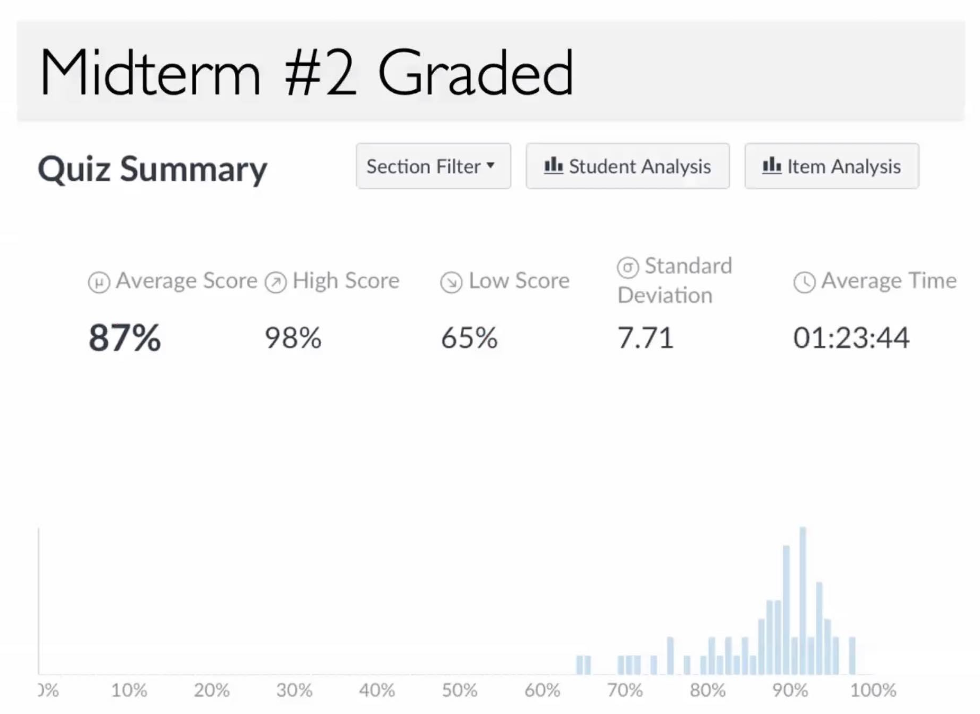
\includegraphics{lectures/wk14/img/mt2_distro.png}

\subsubsection{Regrades}
Same as midterm 1.

\subsubsection{Course Standing}
If you have any concerns about your standing in the
course and your ability to graduate, please get in
touch with us proactively via private message on Ed
Discussion.

\subsection{End of the Semester}
Course summary and next steps on April 27\\
Section: Submit update including demo video this week \textbf{before section}!

\subsection{Design Showcase}
Design Showcase runs Wed-Fri of RRR week every semester. The Jacobs Institute will promote all courses and projects to the public.

Our presentation slot:\\
Design Showcase Session C:\\
Wednesday, 5/3 - 2-3:30pm / Jacobs Hall Room 310

Poster: Due Monday 5/1 11:59am (noon) if you want us to print it!

\subsection{Poster Details}
See \href{https://bcourses.berkeley.edu/courses/1523321/assignments/8584015}{bcourses}.

\subsection{Final Demo Details}
See \href{https://bcourses.berkeley.edu/courses/1523321/assignments/8578979}{bcourses}.

\subsection{Q\&A}
How has ChatGPT changed the way you worked?
\begin{shaded}
Most companies do not allow you to use ChatGPT for obvious reasons but on the side it has been cool to play around with.
\end{shaded}

What courses were most useful?
\begin{shaded}
I work in TypeScript which was not taught in any class at Cal but look into taking DeCals and others, see:
\begin{itemize}
    \item 
\href{https://www.figma.com/proto/LIWnxQaKzQkYD5k5wpP8oA/classes-i've-taken}{https://www.figma.com/proto/LIWnxQaKzQkYD5k5wpP8oA/classes-i've-taken}

    \item 
\href{https://vivrekar.medium.com/discovering-human-computer-interaction-at-uc-berkeley-9fc211145638}{https://vivrekar.medium.com/discovering-human-computer-interaction-at-uc-berkeley-9fc211145638}
\end{itemize}
\end{shaded}

    \section{Thursday, April 18th}
\subsection{Logistics}
\begin{itemize}
    \item Discussion post by Sunday
\end{itemize}

\subsection{Goals}
\begin{itemize}
    \item Channel Capacity w/ and w/o feedback
    \item Joint Typicality (+ AEP)
\end{itemize}

\subsection{Channel Coding Theorem}
If a channel $(\cX, \cY)$
\begin{enumerate}
    \item Discrete: $\cX, \cY$ are discrete.
    \item Memoryless: $Y_i\stackrel{\indep}{\text{given } X_i} \text{ of } y^{(i-1)}, x^{(i-1)}$.
\end{enumerate}
then:
\begin{enumerate}
    \item If $R < C$ then $R$ is achievable.
    \begin{shaded}
        Recall: $R$ is achievable if $\exists$ a set of messages $\cW$. prior $p_\cW$, and encoding $\cC$ s.t. $|\cW|=d^{nR}$\\
        $|C(w)|=n$ (strings length $n$) \underline{and} $\lambda^{(n)}=\max_{w\in
        cW}\{\Pr(\what\neq w\mid \cW = w)\}\stackrel{\to}{n\to\infty}0$
    \end{shaded}
    \item If $R$ is achievable, $R\leq C$. 
    \begin{shaded}
        ($R>C$ is \underline{not} achievable)
    \end{shaded}
\end{enumerate}
where $C=\max_{P_x}\left\{I[X; Y]\right\}$.

We showed last time that $C=1-H[E] = 1 - H([p, 1-p])$, where $E$ indicates an error: $X\neq Y$.

\subsection{Relevant Results in this class}
\begin{enumerate}
    \item Chain Rule: 
    \begin{align*}
        H[X, Y] &= H[X]+H[Y \mid X] \\
        H\left[X^{(\mu)}\right] &= \sum_{i=1}^n H\left[X_1 \mid x^{(1-1)}\right]
    \end{align*}
    \item Joint $\leq$ Sum: $\displaystyle H\left[X^{(n)}\right] \leq \sum_{i=1}^n H\left[X_i\right]$
    \item Data Processing: $X \rightarrow Y \rightarrow W$ then $I[X ; W] \leq I[X ; Y]$
    \item Fano's Inequality: $H[X \mid \hat{x}] \leq 1+P_r(X \neq \hat{x}) \log (|\cX|)$
    \item Conditioning $\searrow$ Uncertainty: $H[X \mid Y] \leq H[X]$ 
    (w/ equality if $\indep$)
\end{enumerate}

\begin{figure}[h]
    \centering
    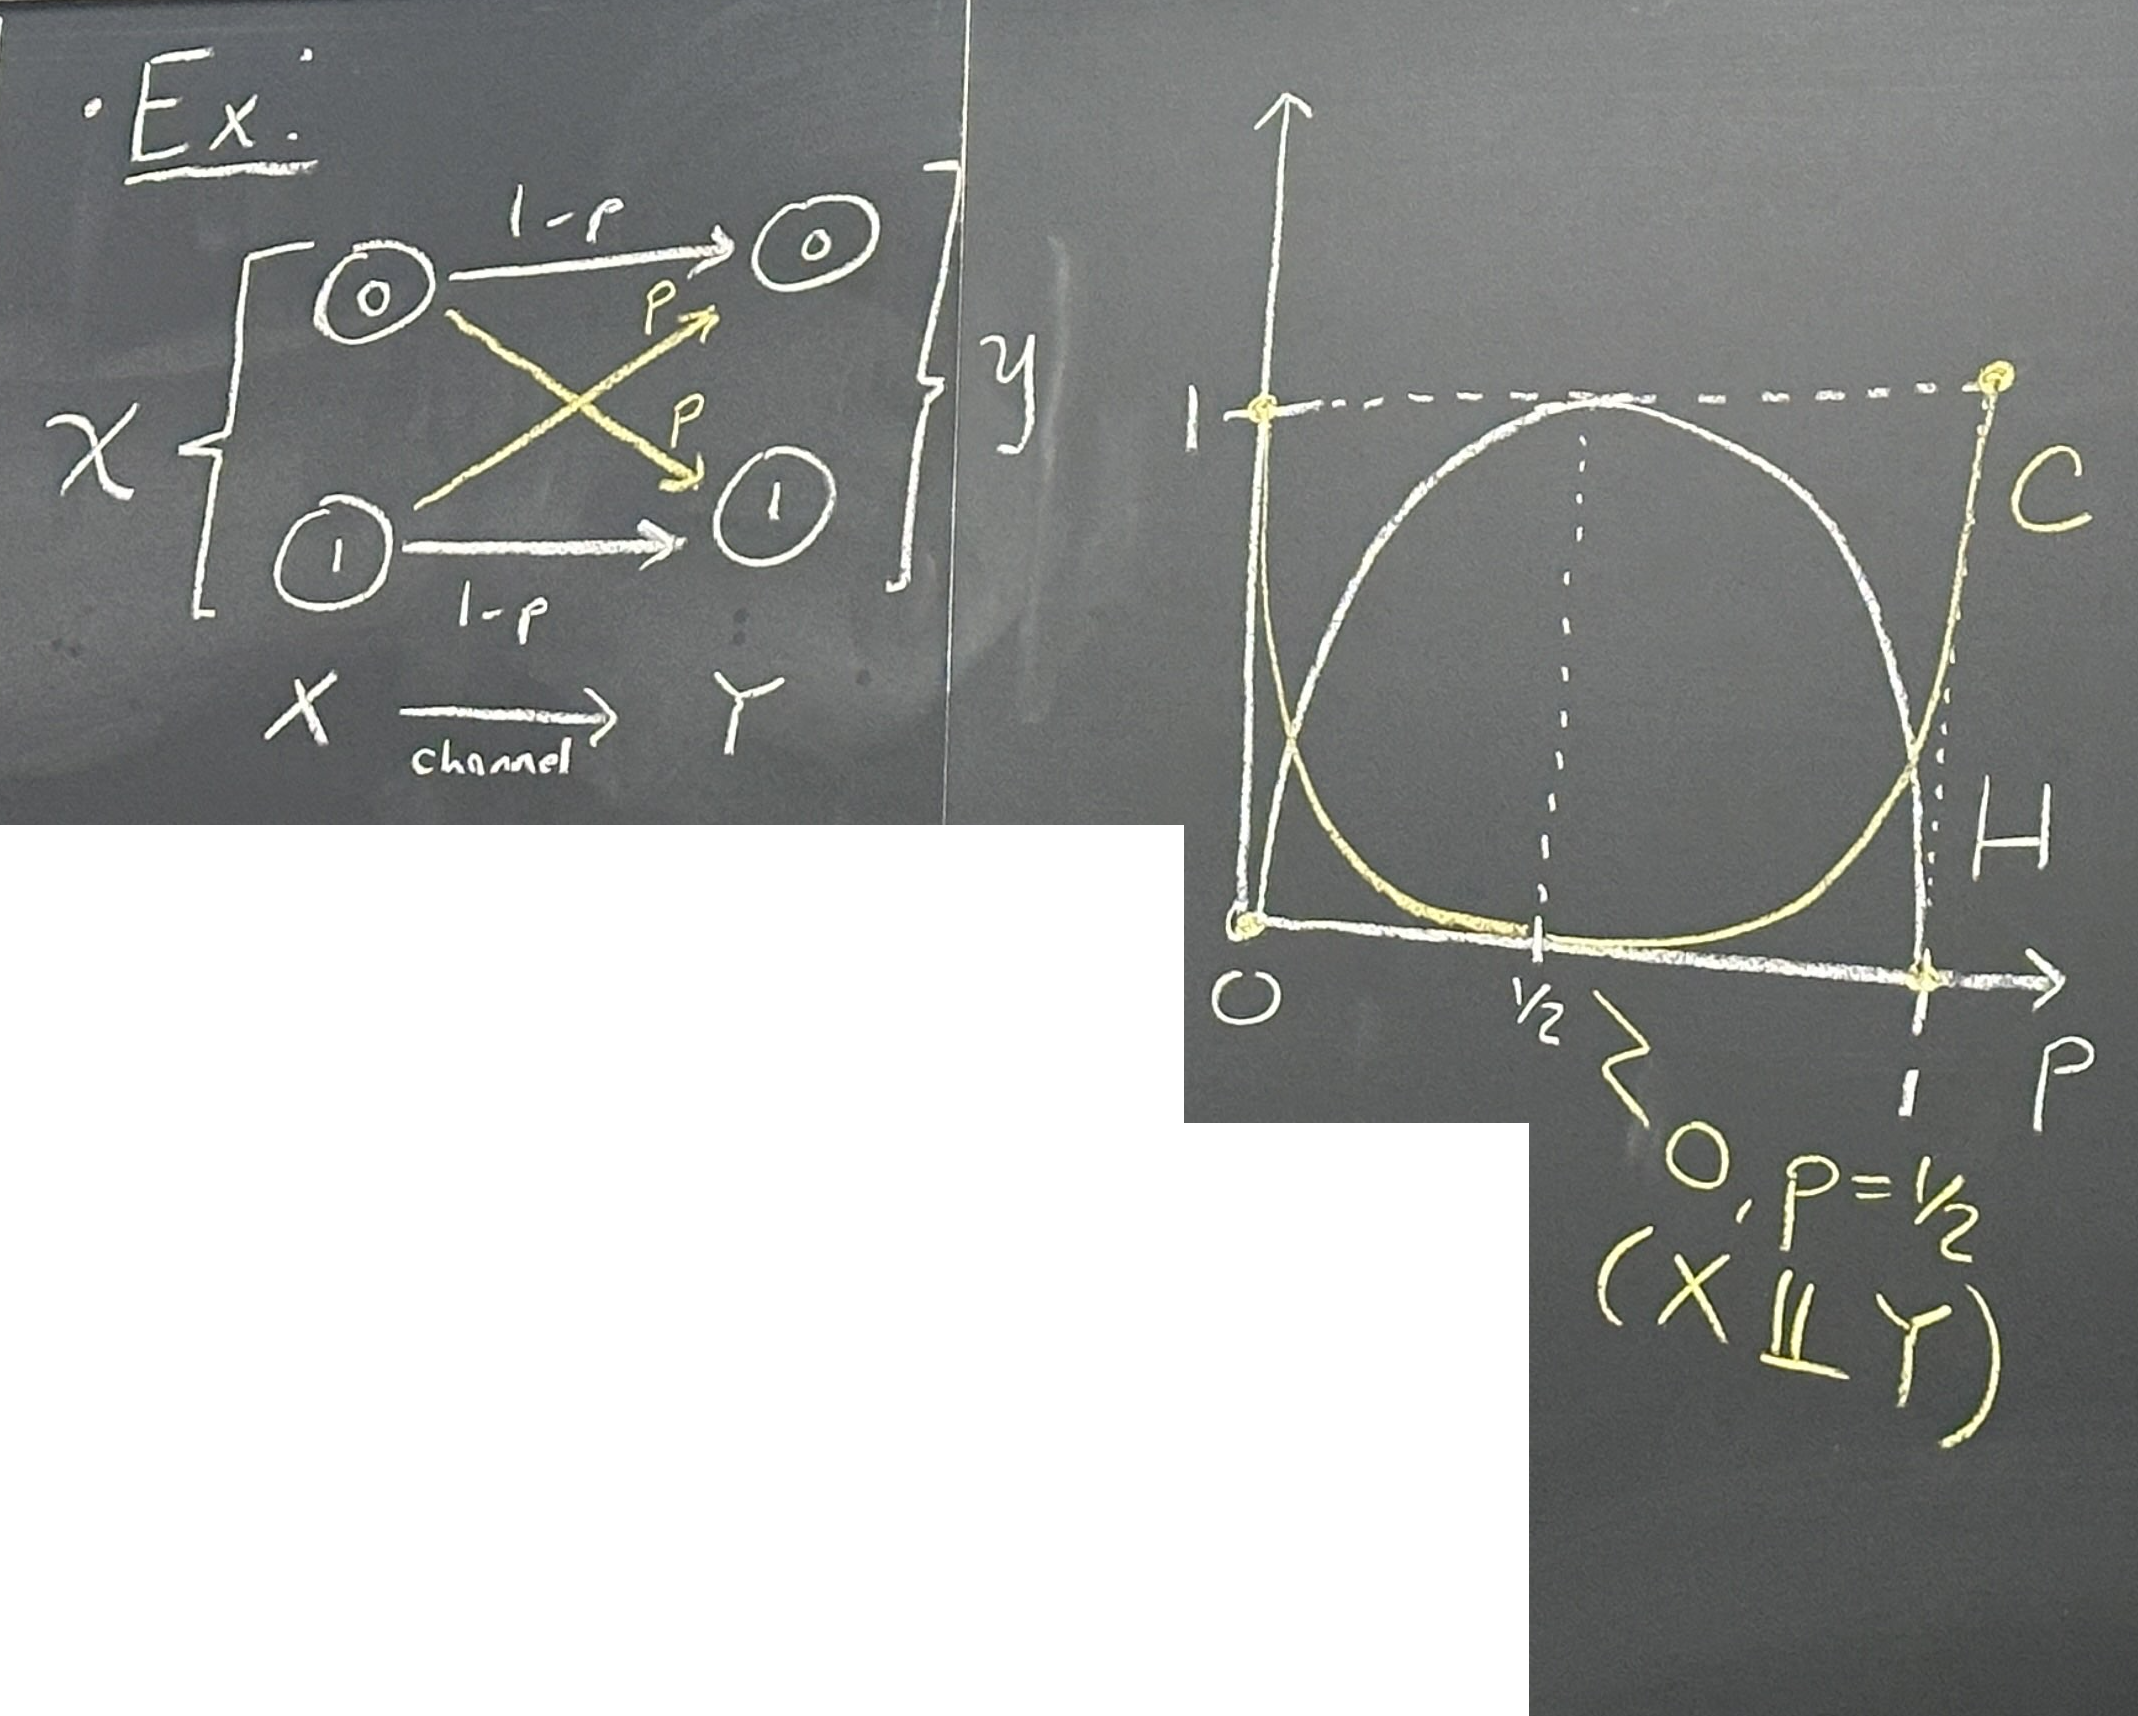
\includegraphics[scale=0.14]{lectures/wk13/img/capacity.png}
    % \caption{Channel Capacity}
    \label{fig:capacity}
\end{figure}

\subsection{The Feedback Capacity Theorem (7.12)}
A channel with feedback is illustrated in the first lecture for this class. We assume that all the received symbols are sent back immediately and noiselessly to the transmitter, which can then use them to decide which symbol to send next. Can we do better with feedback? The surprising answer is no, which we shall now prove. We define a $\left(2^{n R}, n\right)$ feedback code as a sequence of mappings $x_i\left(W, Y^{i-1}\right)$, where each $x_i$ is a function only of the message $W \in 2^{n R}$ and the previous received values, $Y_1, Y_2, \ldots, Y_{i-1}$, and a sequence of decoding functions $g: \mathcal{Y}^n \rightarrow\left\{1,2, \ldots, 2^{n R}\right\}$. Thus,
$$
P_e^{(n)}=\operatorname{Pr}\left\{g\left(Y^n\right) \neq W\right\},
$$
when $W$ is uniformly distributed over $\left\{1,2, \ldots, 2^{n R}\right\}$.
Definition The capacity with feedback, $C_{\mathrm{FB}}$, of a discrete memoryless channel is the supremum of all rates achievable by feedback codes.

Theorem 7.12.1 (Feedback capacity)
$$
C_{\mathrm{F} B}=C=\max _{p(x)} I\left[X ; Y\right].
$$

\begin{Answer}
Proof: Since a nonfeedback code is a special case of a feedback code, any rate that can be achieved without feedback can be achieved with feedback, and hence
$$
C_{\mathrm{FB}} \geq C.
$$

Proving the inequality the other way is slightly more tricky. We cannot use the same proof that we used for the converse to the coding theorem without feedback. Lemma 7.9.2 is no longer true, since $X_i$ depends on the past received symbols, and it is no longer true that $Y_i$ depends only on $X_i$ and is conditionally independent of the future $X$ 's in (7.93).
\end{Answer}

This essentially states that the Channel Coding Thm. is true w/ feedback.

\subsection{Joint Typicality}
Defn.: given $\left(X^{(n)}, Y^{(n)}\right)$, i.i.d from $P_{x^n, Y^n}$ where $P_{x^n, Y^{(n)}}\left(X^{(n)}, Y^{(n)}\right)=\prod_{i=1}^n P_{x, y}\left(x_i, y_i\right)$
\begin{enumerate}
    \item[(i)] $X^{(n)}$ is typical w.r.t.
and $-\frac{1}{n} \log \left(p_{x^n}\left(x^{(n)}\right)\right) \in H L x$ typical w.r.t. $P_y$:
$$
-\frac{1}{n} \log \left(p_{x^n, r^n}\left(x^{(n)}, Y^{(n)}\right)\right) \in H[X, Y] \pm \varepsilon .
$$
\underline{and}
    \item[(iii)] $\left(X^{(n)}, Y^{(n)}\right)$ is typical w.r.t. $p_X$
\end{enumerate}

\begin{figure}[h]
    \centering
    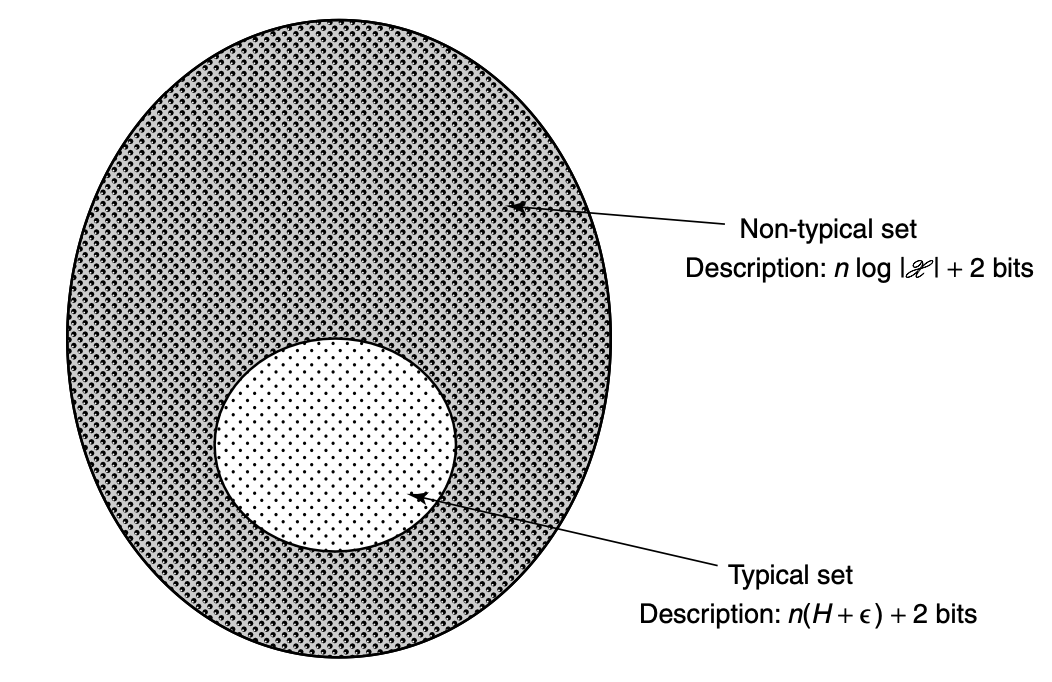
\includegraphics[scale=0.6]{lectures/wk13/img/typical_sets.png}
    \caption{Source code using the typical set shows the Typical set is smaller than any Non-typical set.}
    \label{fig:typical-sets}
\end{figure}

\subsection{Joint AEP}
\begin{enumerate}
\item[(i)] (almost all joint seq. are typical jointly (equipartition))
\begin{equation}
\lim_{n \to \infty} P\left(\left(X^n, Y^n\right) \in A_{\varepsilon}^{(n)}\right) 
= 1. 
\end{equation}

\item[(ii)] $P\left(\left(X^n, Y^n\right) = \left(x^n, y^n\right)\right) \in \leq 2^{-n(H[X,Y]\pm\varepsilon)}, \quad \left(x^n, y^n\right)\in A_{\varepsilon}^n$.

\item[(iii)] 
\begin{align}
\left|A_{\varepsilon}^{(n)}\right| 
    &\leq 2^{n(H[X,Y]+\varepsilon)}
\quad\forall n &&[\text{size is relatively small}]
\\
&\geq (1-\delta)2^{n(H(X,Y)-\varepsilon)}
&&[\text{for $n$ large}]
\end{align}

\item[(iv)] If $\tilde{X}^{(n)}\sim P_{X^n}, \tilde{Y}^{(n)} \sim P_{Y^n}, \tilde{X}^{(n)} \text{ is typical is } \indep \text{ of $\tilde{Y}^{(n)}$ being typical, per (i) and (ii) above: }$ 
\begin{align}
P\left(\left(\tilde X^{(n)}, \tilde Y^{(n)}\right) \in A_{\varepsilon}^{(n)}\right) &\leq 2^{-n(I[X;Y]-3\varepsilon)} \quad &&\forall n 
\\
&\geq (1-\varepsilon)2^{-n(I[X;Y]+3\varepsilon)} \quad &&\text{for } n \text{ large}. 
\end{align}
\end{enumerate}


\subsection{Constructing inequalities}
\begin{itemize}
    \item \# messages: $2^{n R}, \quad$ where $R=\frac{\log_2(|\cW|)}{n}$
    \item Given $X^{(n)}=x^{(n)}: 2^{n H[Y \mid X]}$
    \item Across $2^{n H[Y]} \quad$ typical outcomes
    \begin{align}
    2^{n R} \cdot 2^{n H[Y \mid X]} 
        &\leq 2^{n H[Y]} \\
    R+H[Y \mid X] \leq H[Y], \ 
    &
    R \leq I[X ; Y] \leq C.
    \end{align}
\end{itemize}

\begin{figure}[h]
    \centering
    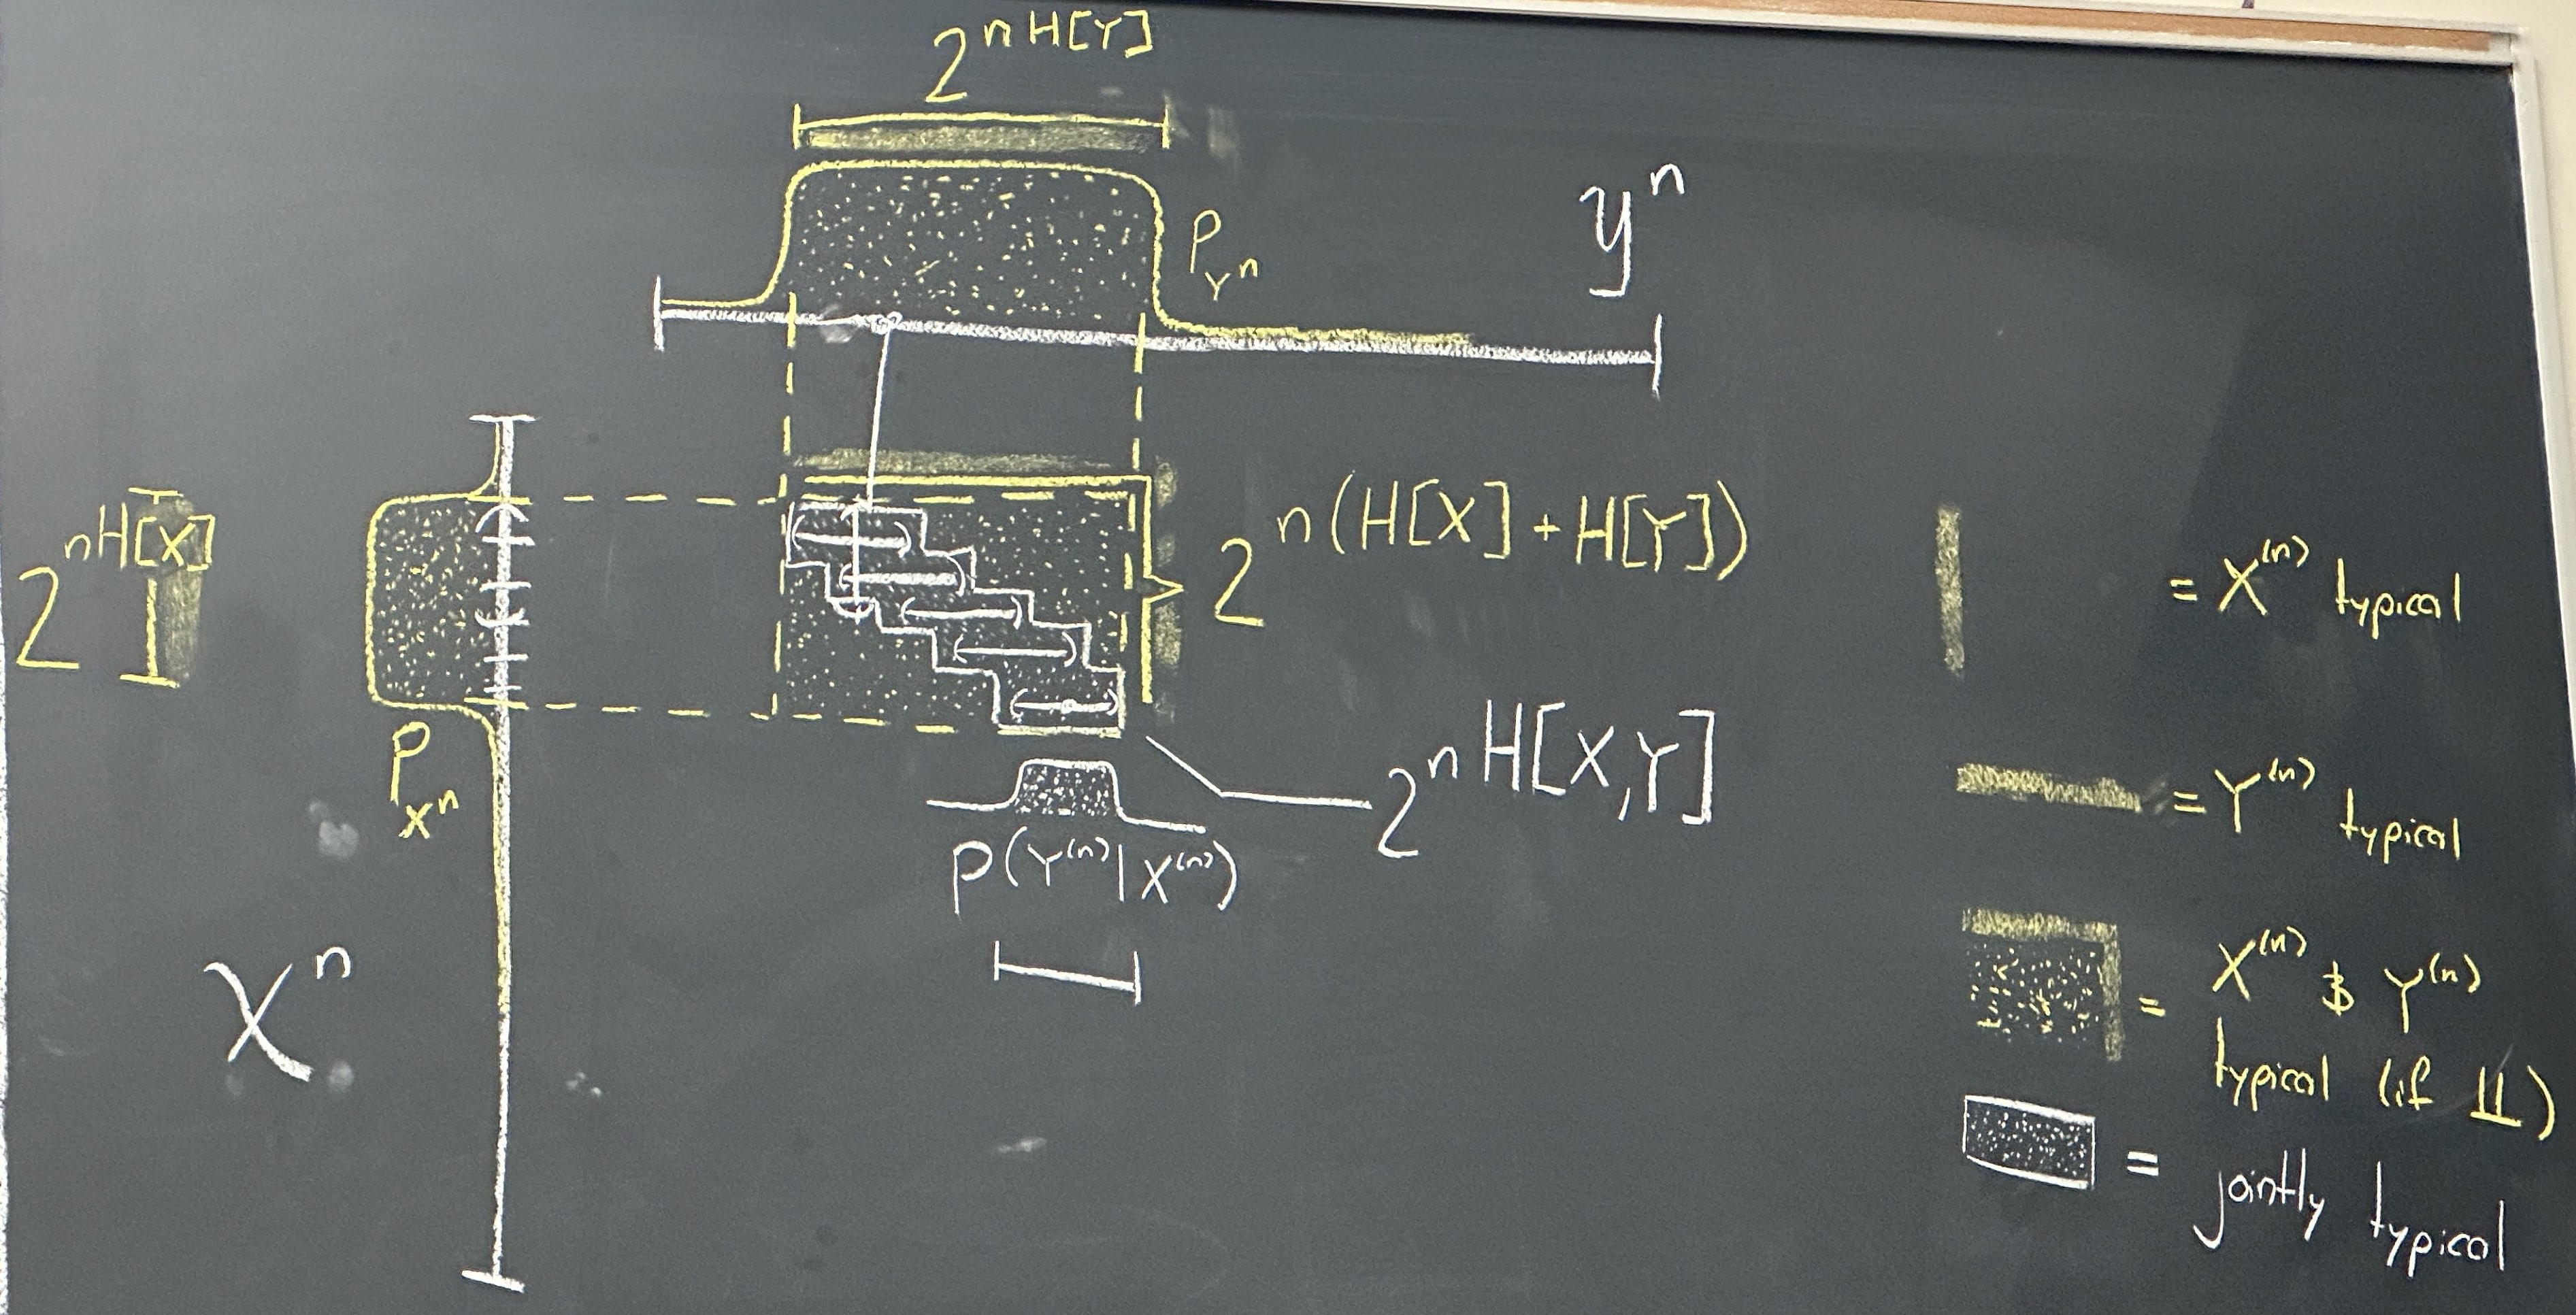
\includegraphics[scale=0.1]{lectures/wk13/img/strip.jpg}
    % \caption{Diagonal Strip}
    \label{fig:strip_firsttime}
\end{figure}

\subsection{Proving that our packing argument is tight}
2. If $R>C$, then $R$ is \underline{not} achievable.\\
If $R$ is achievable then $R \leq C$.
\begin{itemize}
    \item $R$ is achievable $\implies $
    \item Then $P_e^{(i)}=\frac{1}{|\cW|} \sum_w P_r(\hat{w} \neq w \mid W=w) \leq \lambda^{(n)} \longrightarrow 0$
    \begin{itemize}
        \item Consider a model where $W \sim\Uniform({\cW})$
    \begin{equation}
    P_e^{(n)}=\operatorname{Pr}(\hat{w} \neq w) 
    \stackrel{\rightarrow}{{n \rightarrow \infty}}
    0
    \end{equation}
        \item $\implies R \leq C$.
    \end{itemize}
\end{itemize}

\subsection{Putting together Past Relevant Results}
\begin{flalign*}
nR &= \log(|\mathcal{W}|) = H[W] = H\left[W|\What\right] + I\left[W;\What\right] \\
&\leq 1 + P_e^{(n)} \log(|\mathcal{W}|) + I[W;\What] 
&&[\text{Fano's Inequality}]
\\
&= 1 + \underbrace{P_e^{(n)}}_{\to 0 \text{ as } n\to\infty}nR + I[W;\What]
\end{flalign*}
\begin{flalign*}
I\left[W;\underbrace{\What}_{g(Y^{(n)})}\right]
&\leq I\left[W;\hat{Y}^{(n)}\right] = 
H\left[W\right] 
- 
H\left[W|Y^{(n)}\right] 
&&[\text{Data Processing Inequality}] \\
&= I\left[\hat{Y}^{(n)};W\right] 
= H\left[\hat{Y}^{(n)}\right] - H\left[\hat{Y}^{(n)}|W\right]
\end{flalign*}
\begin{flalign*}
H\left[\hat{Y}^{(n)}|W\right] 
&= H\left[Y_1, Y_2, \ldots Y_n \mid W\right] \\
&= \sum_{i=1}^{n} H\left[Y_i^{(n)}|Y^{(i-1)},W\right] &&[\text{Chain Rule}] \\
&=\sum_{i=1}^n H\left[Y_i \mid X_i\right]\\
X_i &= \text{function}(Y^{(i-1)},W) &&[\text{Feedback}] \\
H[Y_i|Y^{(i-1)}, W, X_i] &= H[Y_i \mid X_i] &&[\text{Memoryless}]
\end{flalign*}



    \section{Thursday, April 23rd}
\subsection{Logistics}
\begin{itemize}
    \item Discussion due Thurs
    \item Consulting OH form
    \item Quiz 8 on Thurs (Scope: Last unit up until today, Source Channel Separation Thm.)
\end{itemize}

\subsection{Goals}
\begin{itemize}
    \item Achievability of Capacity
    \item AEP for ergodic sources
    \item Source-Channel Separation
\end{itemize}

\subsection{Channel Coding Theorem}
For a discrete, memoryless channel:
\begin{enumerate}
    \item Any rate $R<C$ is achievable
    \item If $R$ is achievable, then $R\leq C$. (We showed this last time)
\end{enumerate}
where:
$$
C = \max_{P_x} \left\{I[X; Y]\right\}
$$

\begin{proof}
\begin{itemize}
    \item 
All we need is to find a code that achieves $R, R\nearrow C$.
    \item 
Construct a \underline{random code}:
\end{itemize}
\begin{enumerate}
    \item Fix $p_x$
    \item Sample codewords $x^{(n)}(\omega) \{X_i(\omega)\}_{i=1}^n\simiid p_x$. Do this $d^{nR}$ for a base $d$, you have $d$ possible outcomes, to define the codebook.
    \item Sample codewords $x^{(n)}(\omega) \{X_i(\omega)\}_{i=1}^n\simiid p_x$. Do this $d^{nR}$ for a base $d$, you have $d$ possible outcomes, to define the codebook (code): $C$.
    \item Sender \& Receiver know $C, P_{Y|X}$.
    \item $W\sim \Uniform(\cW), \ |\cW|=d^{nR}$.
    \item Encode $W\to X^{(n)}(\omega)$.
    \item Send $X^{(n)}\stackrel{\to}{P_{Y|X}} Y^{(n)}$.
    \item Decode $Y^{(n)}{\to}\what\approx \omega$.
\end{enumerate}
\end{proof}

\subsection{Feedback Capacity Theorem}
The operational capacity w/ feedback is still $C =$ info capacity.

\subsection{Joint AEP Theorem}
$\left(X^{(n)}, Y^{(n)}\right)\sim P_{x^n, y^{(n)}}, \quad \left(X_j, Y_j\right)_{j=1}^n\simiid P_{x, y}$\\
then: 
\begin{enumerate}
    \item[(a)] $\Pr(\left(X^{(n)}, Y^{(n)}\right))$ is j.t. $\to1$ as $n\to\infty$. (almost all sequences $\sim P_{\left(X^{(n)}, Y^{(n)}\right)}$ are j.t.
    \item[(b)] If $\left(x^{(n)}, y^{(n)}\right)$ is j.t. then $\Pr(\left(X^{(n)}, Y^{(n)}\right)=\left(x^{(n)}, y^{(n)}\right))\in d^{-n(H[X, Y] \pm \varepsilon)}$
    \item[(c)] 
    \begin{align*}
    |\text{Jointly typical set}| 
        &\leq d^{n(H[X, Y] + \varepsilon)}
        \\
        &\geq (1-\varepsilon) d^{n(H[X, Y]-\varepsilon)}
        &&\text{ for $n$ large enough}
    \end{align*}
The set of j.t. sequences is (relatively) small.
\item[(d)] If $\tilde{X}^{(n)}\sim p_{x^n}, \tilde{Y}^{(n)}\sim p_{y^n}, \tilde{X}\indep \tilde{Y}$ then: 
\begin{align*}
\Pr(\left(\tilde{X}^{(n)}, \tilde{Y}^{(n)}\right)\text{ is j.t.})
    &\leq d^{-n(I[X; Y] - 3\varepsilon)}
    \\
    &\geq (1-\varepsilon) d^{-n(I[X; Y] + 3\varepsilon)}
        &&\text{ for $n$ large enough}
\end{align*}
$\indep$ly typical sequences are \underline{rarely} j.t.
\end{enumerate}

\begin{figure}[h]
    \centering
    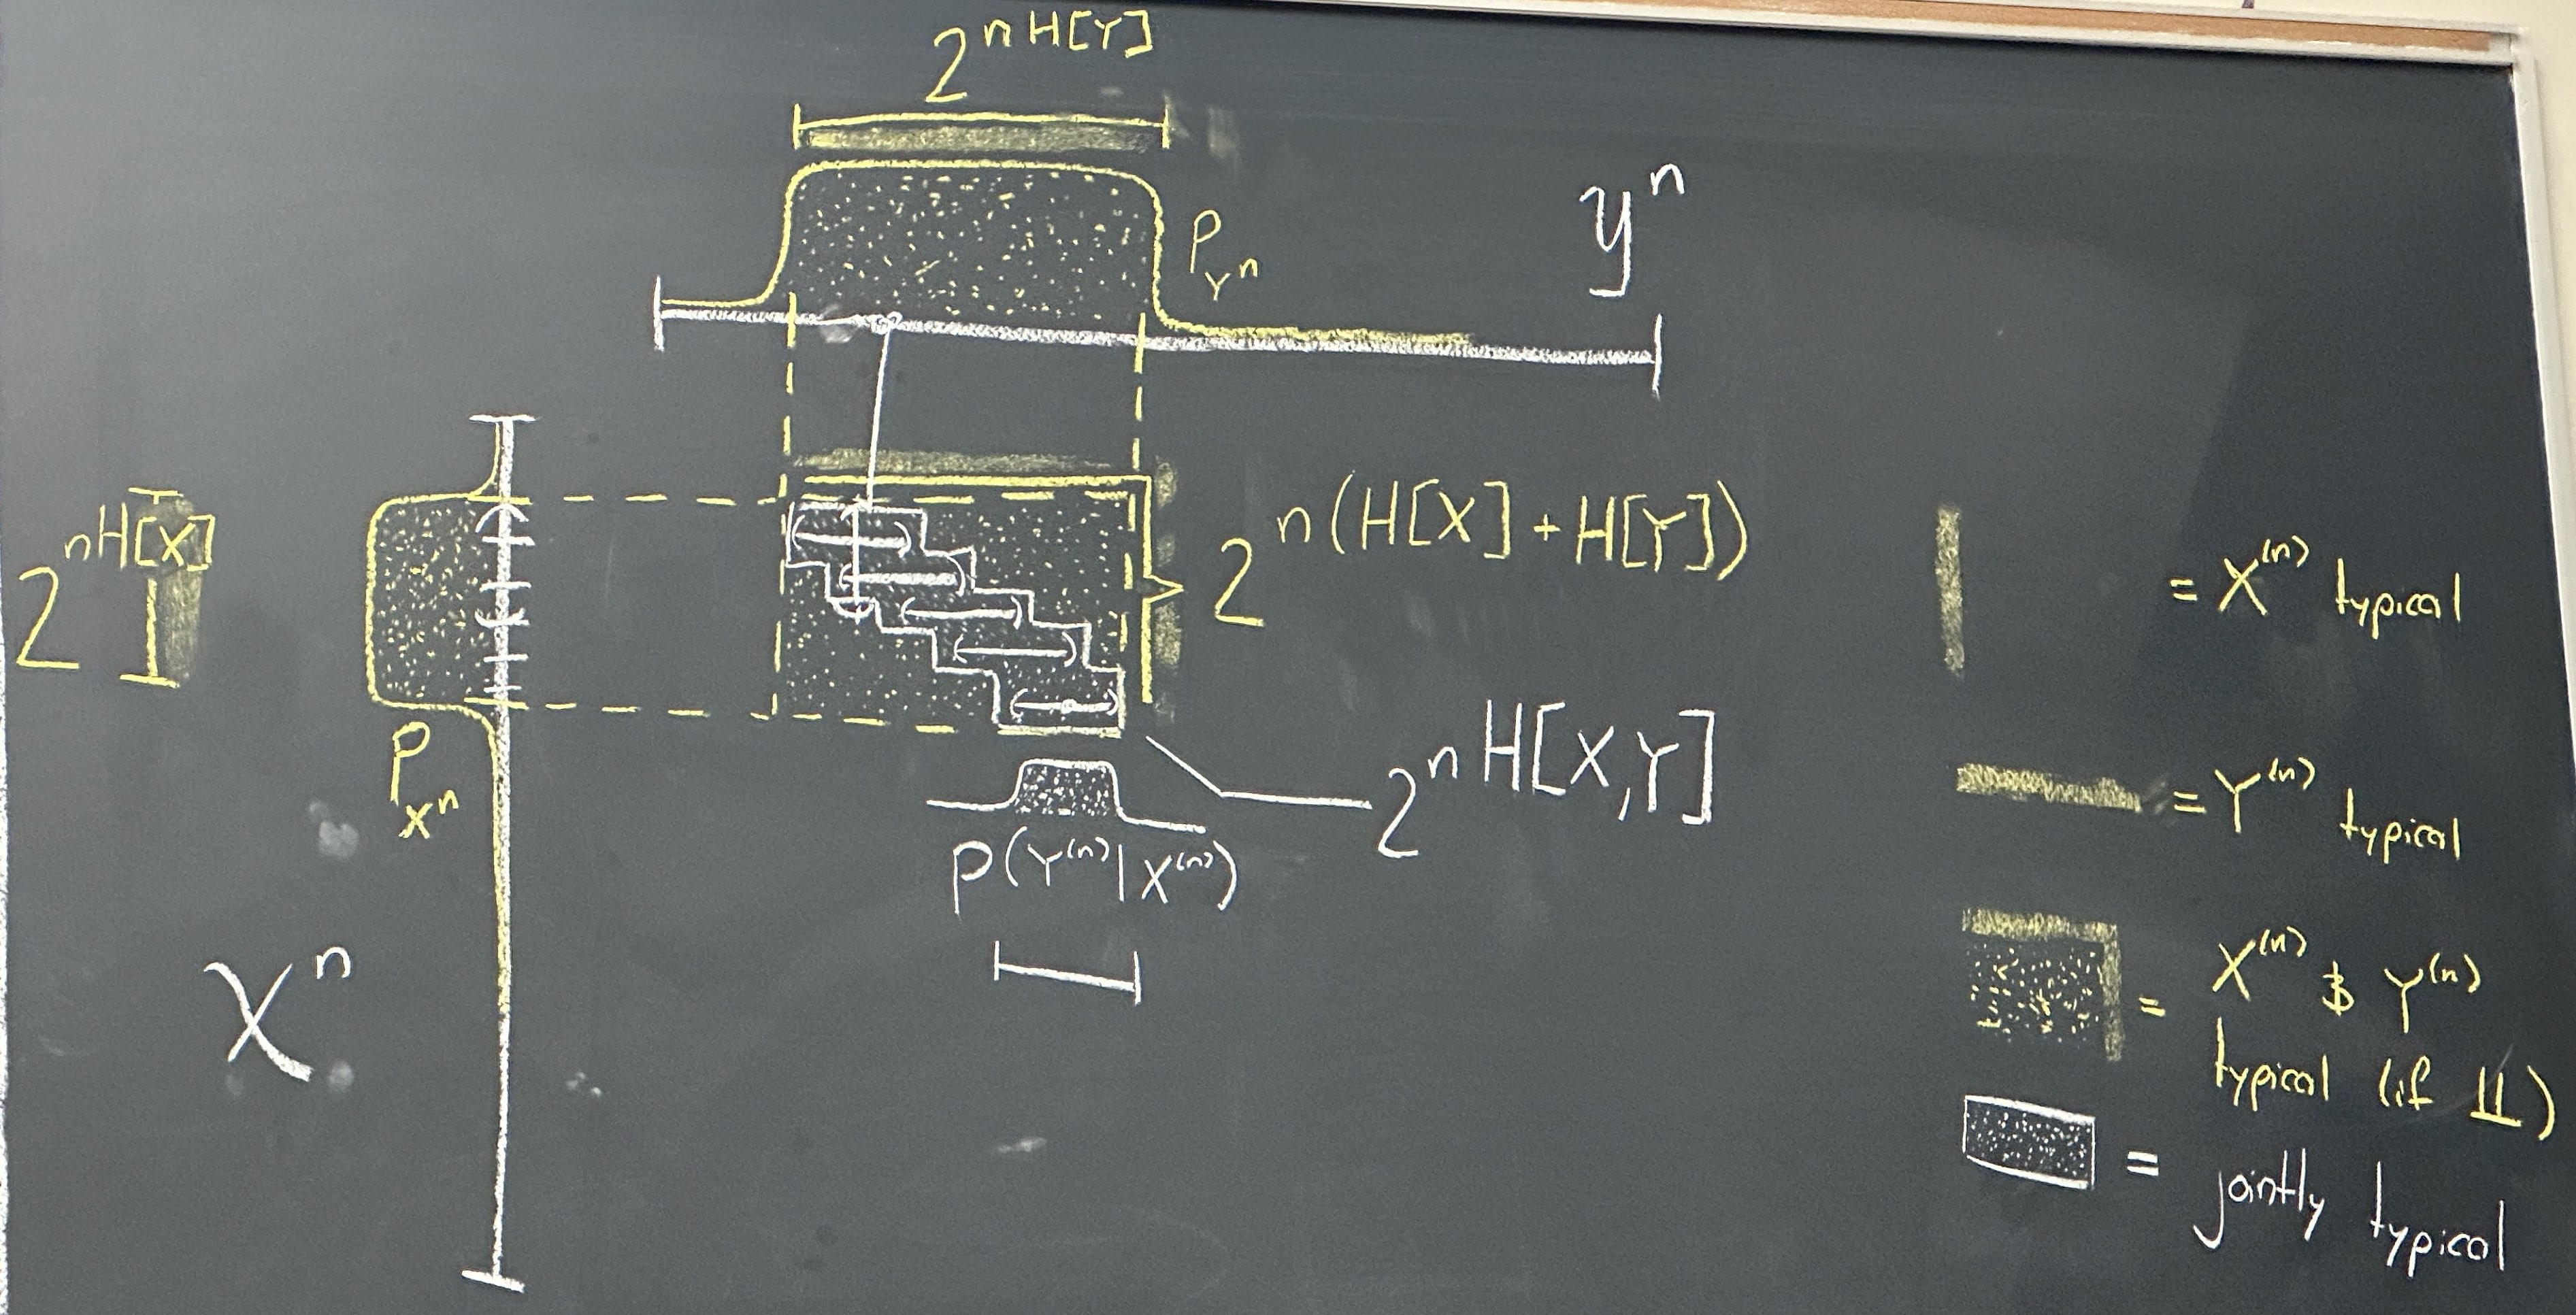
\includegraphics[scale=0.14]{lectures/wk13/img/strip.jpg}
    % \caption{Diagonal Strip}
    \label{fig:strip}
\end{figure}

Here we can see that $\cX^n$ is the input and $y^n$ is the output, we know that we can adjust $\varepsilon$

\subsubsection{How to decode?}
Using j.t., we let $JT(\omega') = \{\left(\tilde{X}^{(n)}(\omega'), \tilde{Y}^{(n)}\right) \text{ is j.t.}\}$.

We decode by looking for an input message $\omega'$ which is j.t. with the received signal $Y^{(n)}$. If there are multiple (we cannot decode properly then we return an error).

\subsubsection{When do we error?}
We error in 2 cases:
\begin{enumerate}
    \item If $JT(\omega)^c=X^{(n)}(\omega)$ is not j.t. w/ $Y^{(n)}$.
    \item If $\exists\omega'\neq\omega\st JT(\omega'), X^{(n)}(\omega')$ is also j.t. with $Y^{(n)}$.
\end{enumerate}

\subsubsection{Detailed Error Analysis}
\begin{flalign*}
\Pr(\text{error}) 
    &= \E_C[\Pr(\text{error} \mid C)] \\
    &= \E_C[\E_W[\Pr(\text{error} \mid C, W)]] \\
    &= \E_{C, W}[\Pr(\text{error} \mid C, W)] \\
    &= \E_{C}[\Pr(\text{error} \mid C, W=1)] \\
    &= \Pr(\text{error} \mid W=1) \\
    &= \Pr(JT(1)^c \cup (\bigcup_{\omega \neq1} JT(\omega)) \mid W=1) \\
    &\leq \underbrace{\Pr(JT(1)^c \mid W=1)}_{\underbrace{Y^{(n)}\text{ is not j.t. w/ } X^{(n)}(1)}_{\leq\varepsilon}}
    + \sum_{\omega \neq1}\Pr(JT(\omega') \mid W=1) 
    &&[\text{Apply Union Bound}] \\
    \Pr(JT(1)^c \mid W=1)
        &\leq \varepsilon \text{ for large } n
    &&[\text{by AEP}] \\
    % \implies \Pr(\text{error}) &\leq \varepsilon + \sum_{\omega \neq1}\Pr(\underbrace{JT(\omega') \mid W=1}_{\underbrace{\stackrel{W=1\to X^{(n)}(1)\to Y^{(n)}}{\omega'\neq 1\to X^{(n)}(\omega')}}_{\left(\tilde{X}^{(n)}(\omega'), \tilde{Y}^{(n)}\right)\text{ drawn }\indep\text{ly of }X^{(n)}(1), X^{(n)}(\omega')\indep Y^{(n)} \text{ if }\omega'\neq1}) \\
        &\leq \varepsilon +\sum_{\omega'\neq1} d^{-n(I[X; Y] -3\varepsilon)} \\
        &\leq \varepsilon +\sum_{\omega'\neq1} d^{nR} d^{-n(I[X; Y] -3\varepsilon)} \\
        &\leq \varepsilon +\sum_{\omega'\neq1} d^{-n((I[X; Y] -3\varepsilon) - R)}
\end{flalign*}
If $R < I[X; Y]-3\varepsilon$ then $d^{-n(\ldots)}\searrow0$ as $n\to\infty$. If $R < I[X; Y]-3\varepsilon, \exists n$ large enough $\st\Pr(\text{error})\leq 2\varepsilon$.

\subsection{Source Model}
Suppose $\cW$ is a stochastic process. 
\begin{align*}
    W^{(n)}=\{W_i\}_{i=1}^n\sim\cW
\end{align*}
This is producing new entropy every time I draw sample, which makes us take more to encode the information.

First extend the AEP to apply to stochastic sources: Recall that the AEP is, in essence, LLN. This means we can consider \underline{ergodic} (stationary) sources, where ergodic means that if we take a sample average over trajectories, it will be close to the population average.
\begin{align*}
    \lim_{T\to\infty}\frac{1}{T}\sum_{t=1}^{T} f(W_t) \ip \E_{W\sim P_s}[f(W)]
\end{align*}

\subsection{AEP: Shannon–McMillan–Breiman Theorem}
If $H$ is the entropy rate of a finite-valued stationary ergodic process $\left\{X_n\right\}$, then
$$
-\frac{1}{n} \log p\left(X_0, \ldots, X_{n-1}\right) \rightarrow H \quad \text { with probability } 1 .
$$

\subsection{Source-Separation Theorem}
Extension to the Channel Coding Theorem for Source: if given a stochastic source which satisfies the AEP, then we can transmit messages with vanishingly probability of error.

If $V_1, V_2, \ldots V^n$ is a finite alphabet stochastic process that satisfies the AEP and $H(\mathcal{V})<$ $C$, there exists a source-channel code with probability of error $\operatorname{Pr}\left(\hat{V}^n \neq\right.$ $\left.V^n\right) \rightarrow 0$. Conversely, for any stationary stochastic process, if $H(\mathcal{V})>C$, the probability of error is bounded away from zero, and it is not possible to send the process over the channel with arbitrarily low probability of error.

\subsection{What we have shown}
If $R<I[X ; y]-3 \varepsilon$, then for large $n$, average $P(\text{error})\leq 2\varepsilon$.

1. Use $P_x=P_x^*=\underset{P_x}{\operatorname{argmax}}\{I[X ; Y]\}$ then $I[X ; Y]=C$ then if $R<C$, average prob of error $\rightarrow 0$ as $n\to\infty$.

2. $\Pr(\text{error})=\mathbb{E}_{C}\left[P(\text{error} \mid C)\right] \leq 2 \varepsilon$ then $\exists C^\ast\st\Pr(\text{error}\mid C^\ast)\leq 2\varepsilon$.

3. \begin{align*}
\operatorname{Pr}\left(\text{error} \mid C^\ast\right) &\leq 2 \varepsilon.
\\
\operatorname{Pr}\left(\text{error} \mid C^\ast\right)
    &=\mathbb{E}_{W \sim \text{ Uniformly}(\cW)}\left[\operatorname{Pr}\left(\text{error} \mid C^\ast, W\right)\right] \leq 2 \varepsilon.
\end{align*}
There exists a set of messages $W\st\Pr(\text{error}\mid C^\ast, W)\leq 4\varepsilon$ and there are at least $|\cW|/2=\frac{2^{nR}}{2}=2^{nR-1}=2^{n(R-1/n)}$ and discard all other messages.

Provided $\displaystyle\lim _{n \rightarrow \infty} R^{\prime}=\lim _{n \rightarrow \infty}(R - 1 / n)<C$.



    \section{Thursday, April 25th}
\subsection{Logistics}
\begin{itemize}
    \item Slip days with partners is the $\max$
    \item Quiz 8 today + retakes
    \item Project due Monday after reading week
    \item Consulting OH form is now live
\end{itemize}

\subsection{Wrap-Up Activity}
For each of the following, discuss:
\begin{enumerate}
    \item Something you learned that:
    \begin{enumerate}
        \item You found surprising, clarifying, important, useful
        \item You would like to remember/tell a friend
    \end{enumerate}
    \item Something you found confusing (to clarify)
    \item Something you'd like to learn next
\end{enumerate}

\subsubsection{Foundations}
\subsubsection{Entropy}
\begin{itemize}
    \item Entropy as expected surprise/entropy intuition.
\end{itemize}

\subsubsection{Information}
\begin{itemize}
    \item Why KL Divergence is not symmetric, taking one to be the null hypothesis (ground assumption): the order of input matters and why this is a feature and not a bug. Specifically, instead of thinking of it as measuring distance, think of how distinguishable the 2 distributions are. It is not symmetric to say how distinguishable $P$ is from $Q$ is the same as $Q$ from $P$.
    \item In the past, it was just a tool to measure things and used bluntly without thought on why. This class was offered to give intuition to motivate its use in many problems.
    \item The Chernoff-Stein Lemma tells us that the KL Divergence is the rate of decay for how much data do you need to quantify probability of error as small enough.
\end{itemize}

\subsubsection{Processes}
\subsubsection{Communication}
\begin{itemize}
    \item For a discrete memoryless channel Feedback doesn't help (asymptotically).
    \item Appreciation of Architecture.
\end{itemize}

\subsection{Looking Ahead}
\begin{itemize}
    \item Kolmogorov Complexity (more of a CS topic so not focused on here, see CS 70)
    \item Variational Principles for Divergences (more of a STAT 210B topic)
    \item Application to (Kelly) Betting with $\log$ growth rates of evidence (more of a STAT 165 topic).
    \item Utility of perfect information: Information Markets (more of a CS 188 topic).
    \item Estimating Information especially in high-dimensional (intractable) space (more of a DATA C102 topic).
\end{itemize}

\end{document}
